\chapter{List of Scans} \label{scans}

\Cref{tab:params} lists the scan parameters of the 25 named scans, which are presented in the following. The parameters are: sweep time, sensor orientation (\textbf{H}orizontal / \textbf{V}ertical / \textbf{H}orizontal \textbf{I}nverted beam fan), squint angle (center of sensor's FOV, so \ang{90} is sideways-looking and \ang{0} is forward-looking), mounted horn antenna extension (which narrows the beam shape), availability of \texttt{/map} rosmessages with lidar slam information, and finally availability of \texttt{/tf} rosmessages which carry the slam-based odometry drift correction.

\begin{table}[htb]
  \caption{Scan parameters}
  \label{tab:params}
  \rowcolors{1}{ColorAlternatedRow}{}
    \begin{tabularx}{\textwidth}{%
      >{\setlength{\hsize}{.31\hsize}\raggedright\arraybackslash}X%
      >{\setlength{\hsize}{.15\hsize}\raggedright\arraybackslash}X%
      >{\setlength{\hsize}{.12\hsize}\raggedright\arraybackslash}X%
      >{\setlength{\hsize}{.12\hsize}\raggedright\arraybackslash}X%
      >{\setlength{\hsize}{.10\hsize}\centering\arraybackslash}X%
      >{\setlength{\hsize}{.10\hsize}\centering\arraybackslash}X%
      >{\setlength{\hsize}{.10\hsize}\centering\arraybackslash}X%
    }
    \hiderowcolors
    \toprule
Name & Sweep & Orient. & Squint & Horn & Map & TF \\
    \midrule
    \endhead

    \bottomrule
    \endfoot
    \showrowcolors
    %
 Attic & \SI{5.0}{ms} & H & \ang{90} & \cmark & \xmark & \xmark \\
 Basement & \SI{5.0}{ms} & H & \ang{90} & \cmark & \xmark & \xmark \\
 Cafeteria & \SI{5.0}{ms} & H & \ang{90} & \cmark & \xmark & \xmark \\
 Dungeon & \SI{5.0}{ms} & V & \ang{20} & \cmark & \xmark & \xmark \\
 Entryway & \SI{5.0}{ms} & V & \ang{20} & \cmark & \xmark & \xmark \\
 Fallout Shelter & \SI{5.0}{ms} & V & \ang{20} & \cmark & \xmark & \xmark \\
 Garden & \SI{5.0}{ms} & V & \ang{20} & \cmark & \xmark & \xmark \\
 Home Cinema & \SI{5.0}{ms} & V & \ang{20} & \cmark & \xmark & \xmark \\
 Indoor Swimming Pool & \SI{5.0}{ms} & V & \ang{20} & \cmark & \xmark & \xmark \\
 Jail Cell & \SI{5.0}{ms} & H & \ang{20} & \cmark & \xmark & \xmark \\
 Kitchen & \SI{5.0}{ms} & H & \ang{20} & \xmark & \xmark & \xmark \\
 Lobby & \SI{5.0}{ms} & H/I & \ang{0} & \xmark & \xmark & \xmark \\
 Mancave & \SI{5.0}{ms} & H/I & \ang{0} & \xmark & \xmark & \xmark \\
 Nirvana & \SI{5.0}{ms} & H/I & \ang{0} & \xmark & \cmark & \xmark \\
 Orbit & \SI{5.0}{ms} & H/I & \ang{0} & \xmark & \cmark & \xmark \\
 Public Restroom & \SI{5.0}{ms} & H/I & \ang{0} & \xmark & \cmark & \cmark \\
 Queue & \SI{20}{ms} & H/I & \ang{0} & \xmark & \cmark & \cmark \\
 Racetrack & \SI{2.0}{ms} & H/I & \ang{0} & \xmark & \cmark & \cmark \\
 Sauna & \SI{2.5}{ms} & H/I & \ang{0} & \xmark & \cmark & \cmark \\
 Torture Chamber & \SI{2.5}{ms} & H/I & \ang{45} & \xmark & \cmark & \cmark \\
 Underground & \SI{2.5}{ms} & H/I & \ang{45} & \xmark & \cmark & \cmark \\
 Virtual Reality & \SI{2.5}{ms} & H/I & \ang{45} & \xmark & \cmark & \cmark \\
 Washroom & \SI{2.5}{ms} & V & \ang{45} & \xmark & \cmark & \cmark \\
 Xray-Room & \SI{2.5}{ms} & V & \ang{0} & \xmark & \cmark & \cmark \\
 Y Is There A Cable On The Floor & \SI{5.0}{ms} & V & \ang{0} & \xmark & \cmark & \cmark \\
%  Z & & & & & & \\
    \end{tabularx}
\end{table}



\begin{figure}[htbp]
    \centering
    \begin{subfigure}[t]{0.475\linewidth}
        \centering
        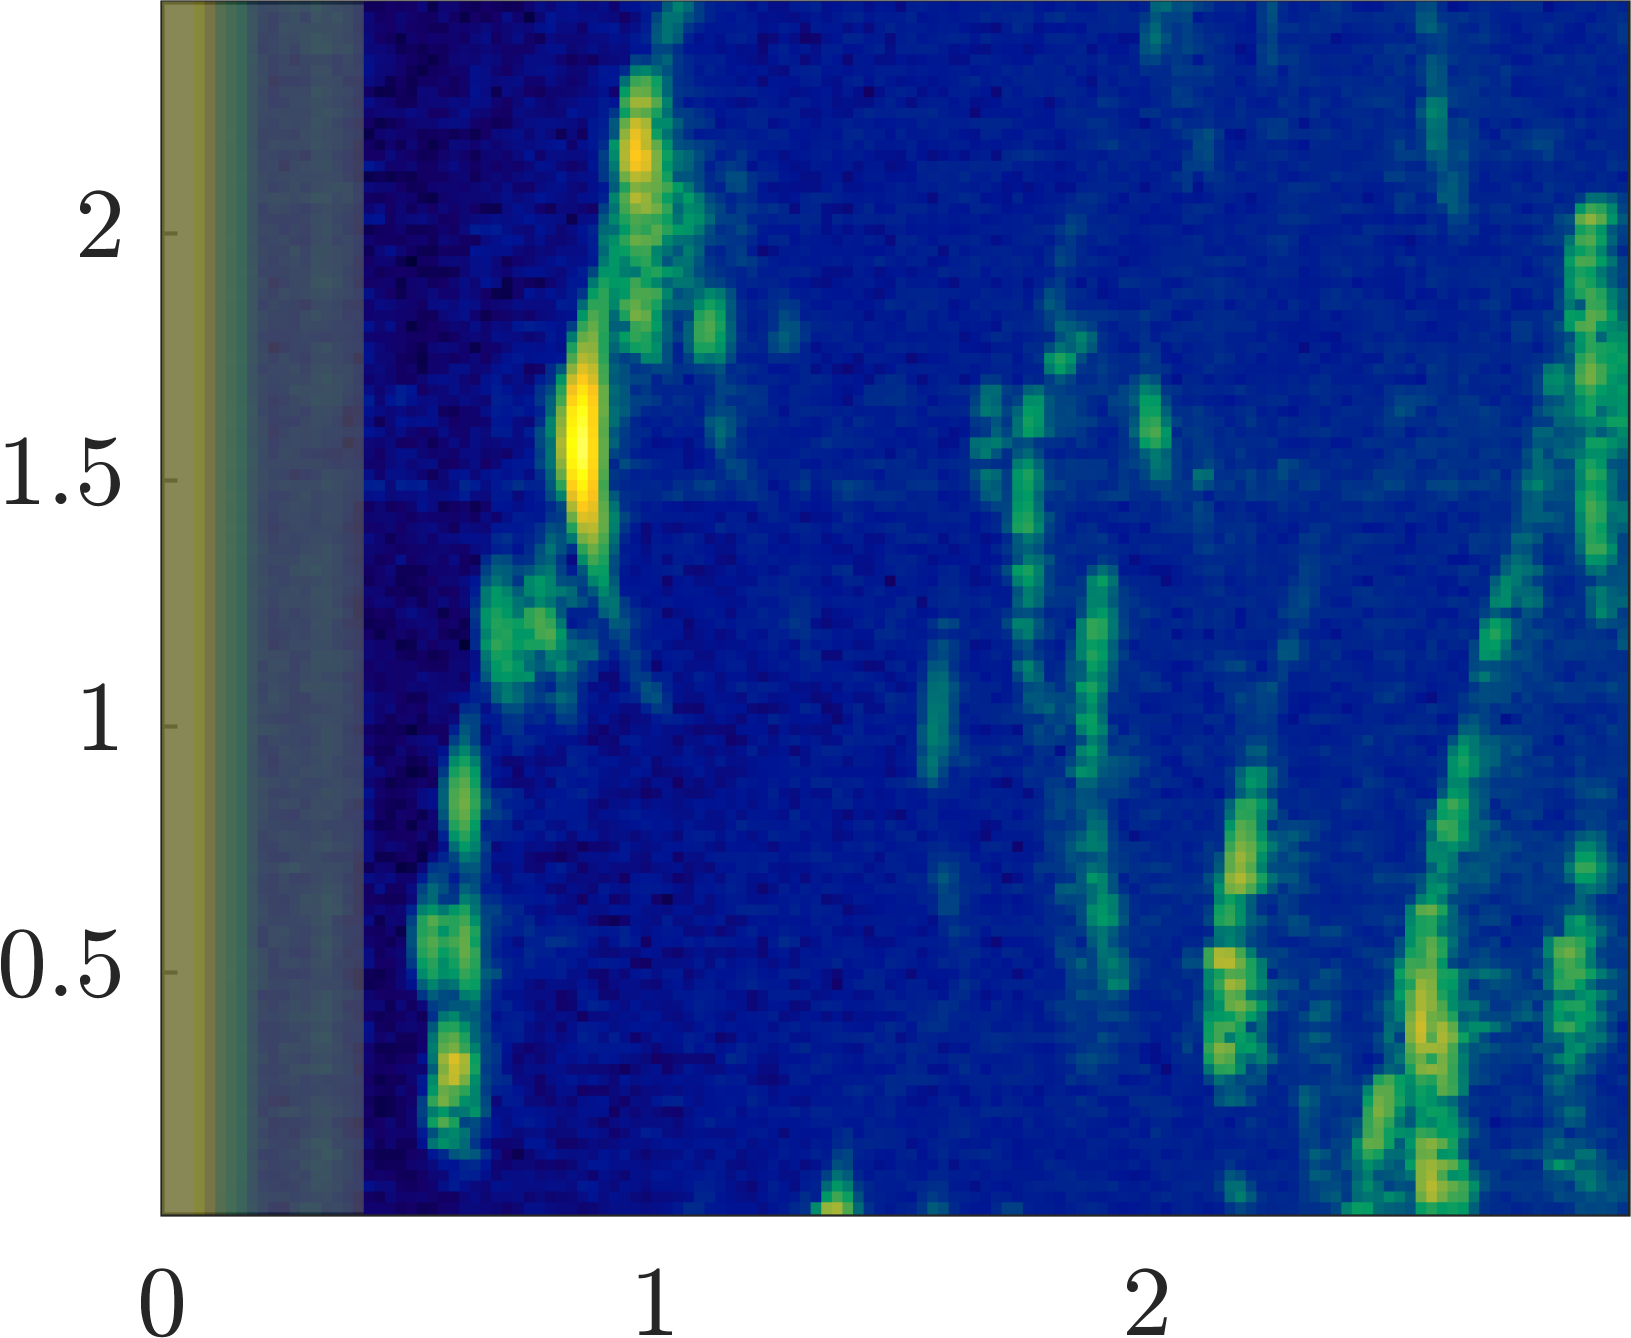
\includegraphics[width=\linewidth,max height=.475\textheight]{gfx/results/attic_input.png}
    \end{subfigure}%
    \hfill%
    \begin{subfigure}[t]{0.475\linewidth}  
        \centering 
        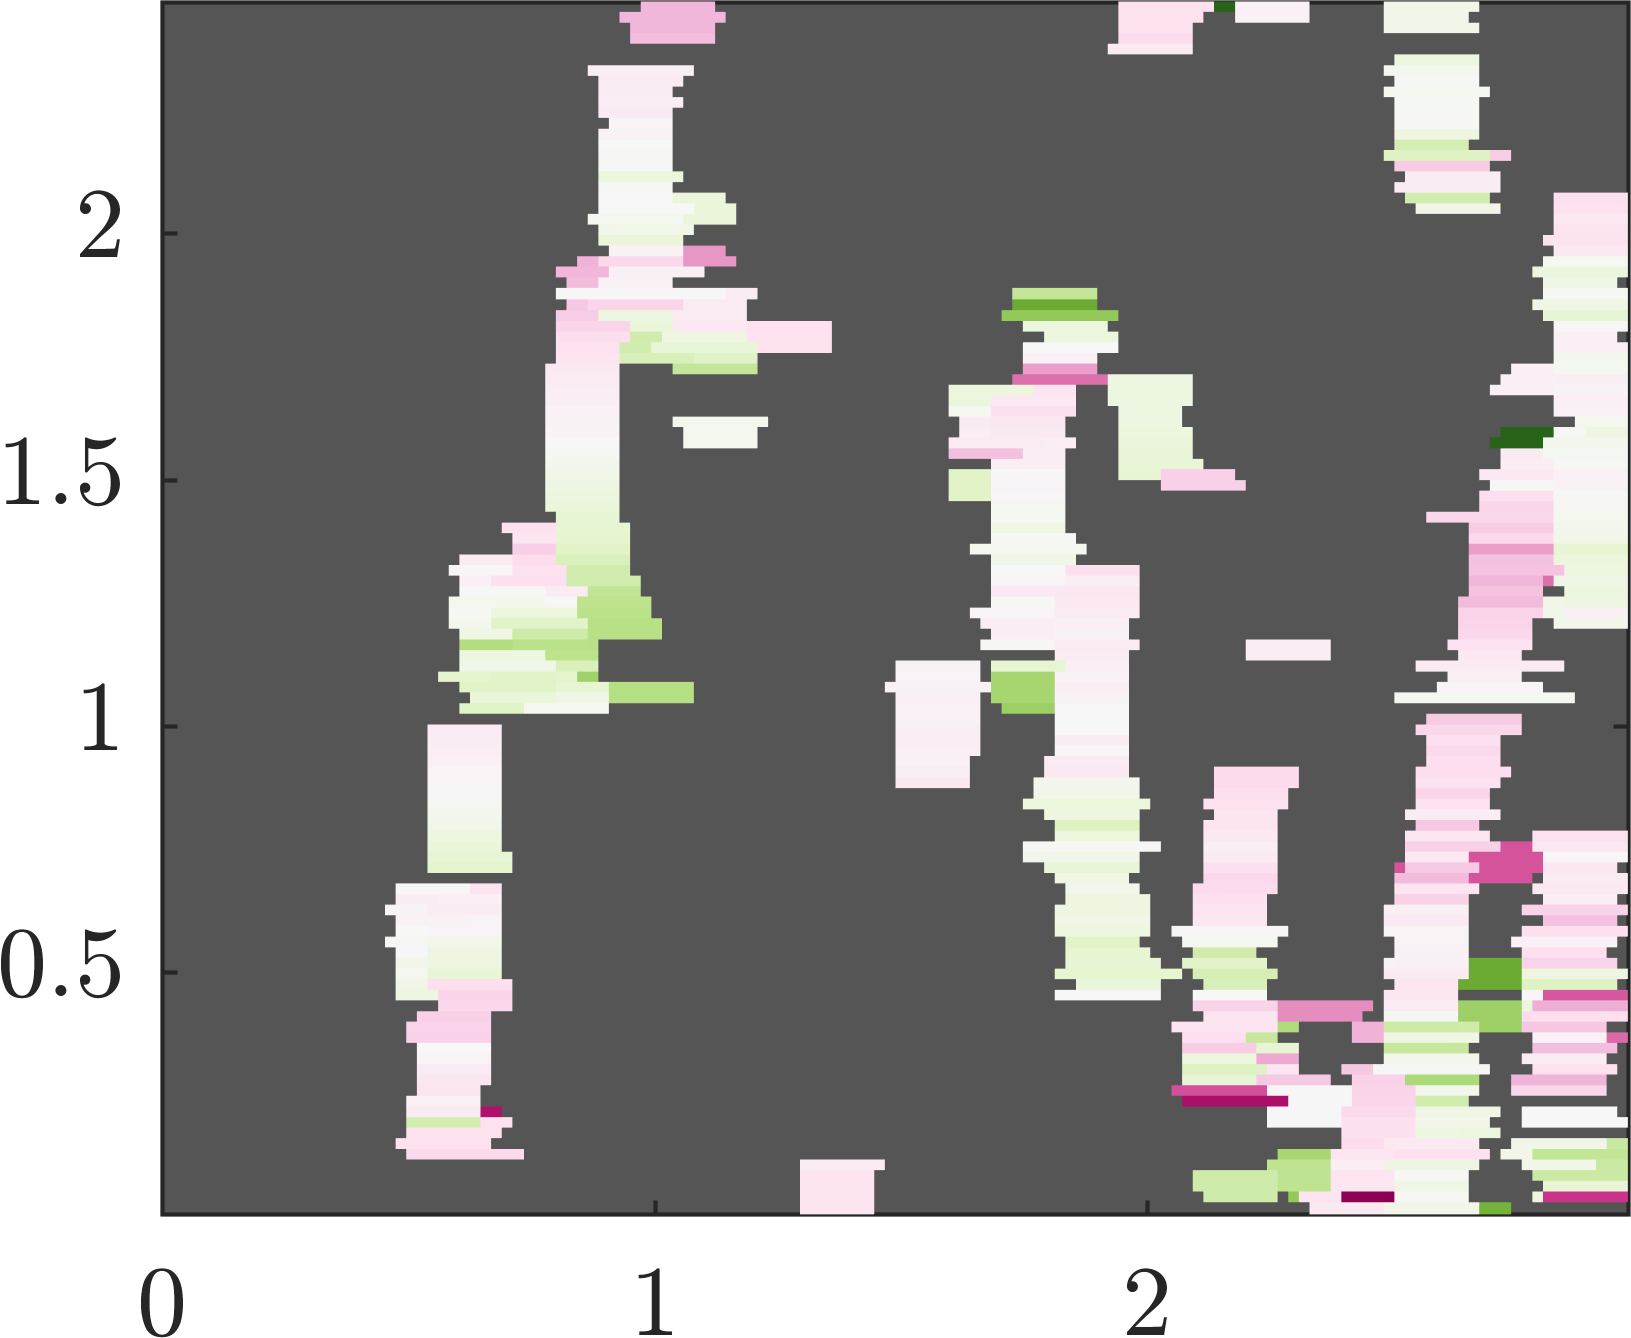
\includegraphics[width=\linewidth,max height=.475\textheight]{gfx/results/attic_doppler.png}
    \end{subfigure}\bigskip\\
    \begin{subfigure}[t]{0.5\linewidth}   
        \centering 
        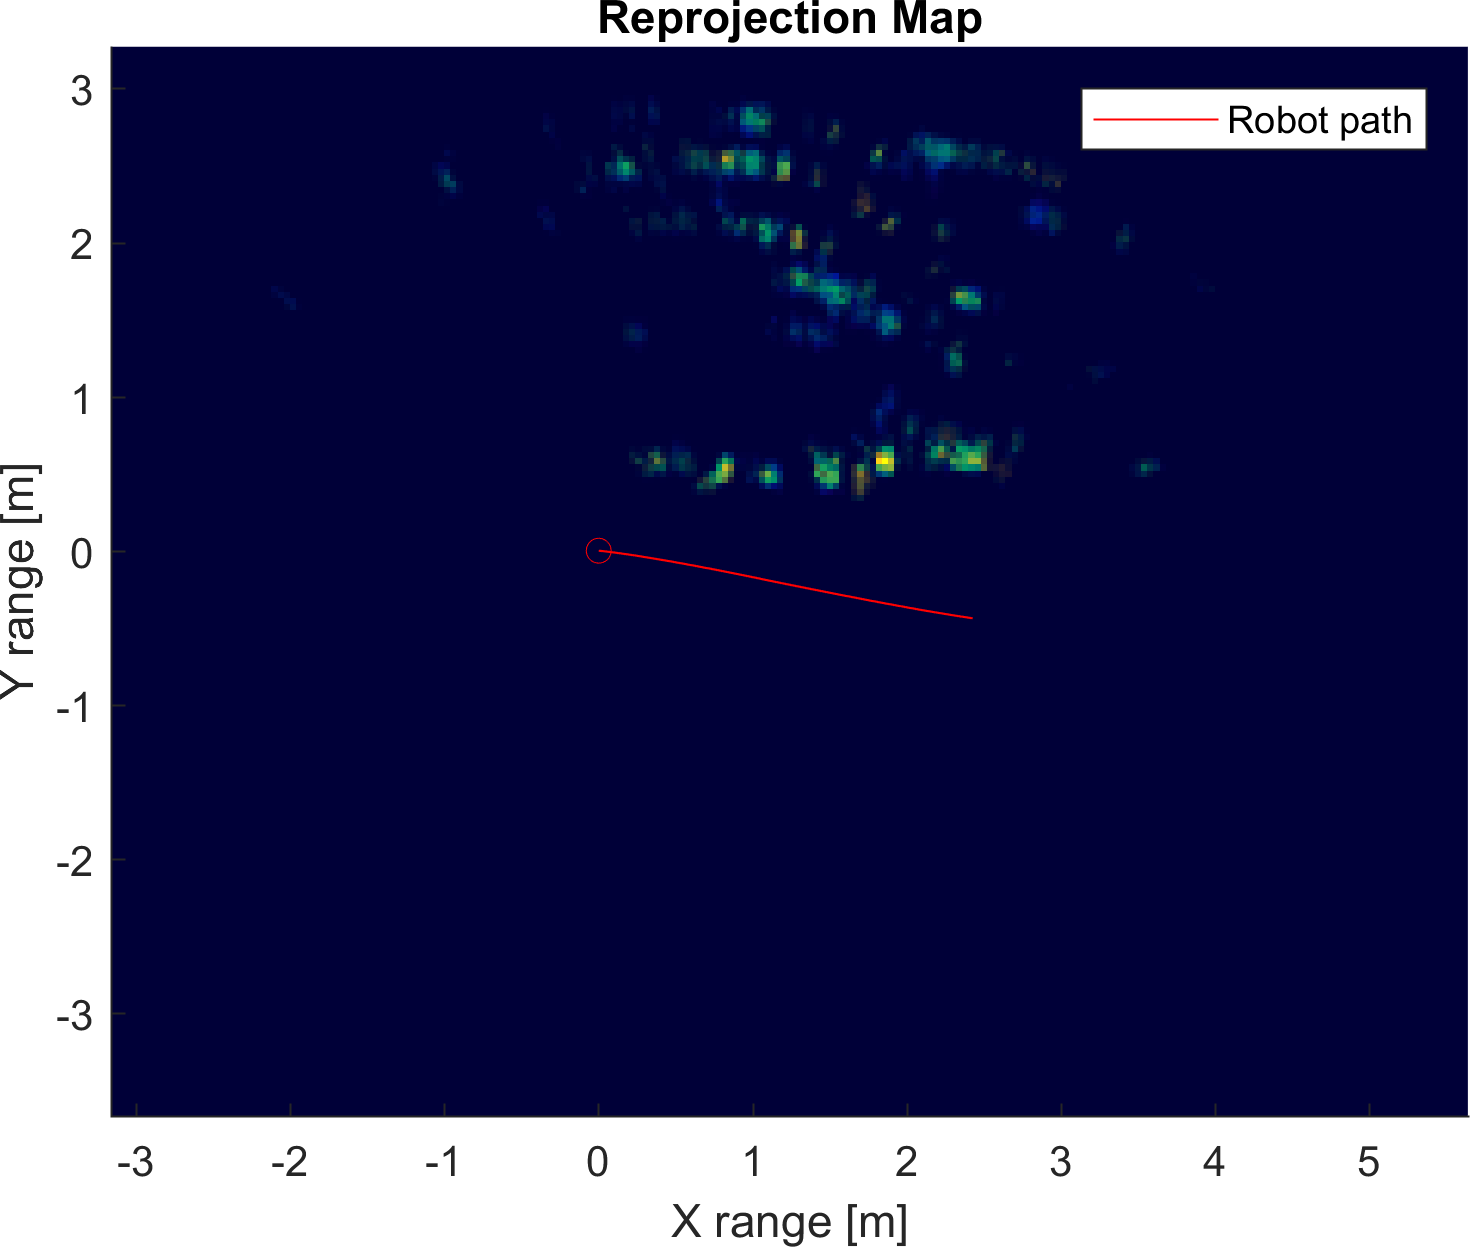
\includegraphics[width=\linewidth,max height=.475\textheight]{gfx/results/attic_reprojection.png}
    \end{subfigure}%
    \caption{Attic scan}
\end{figure}

\begin{figure}[htbp]
    \centering
    \begin{subfigure}[t]{0.475\linewidth}
        \centering
        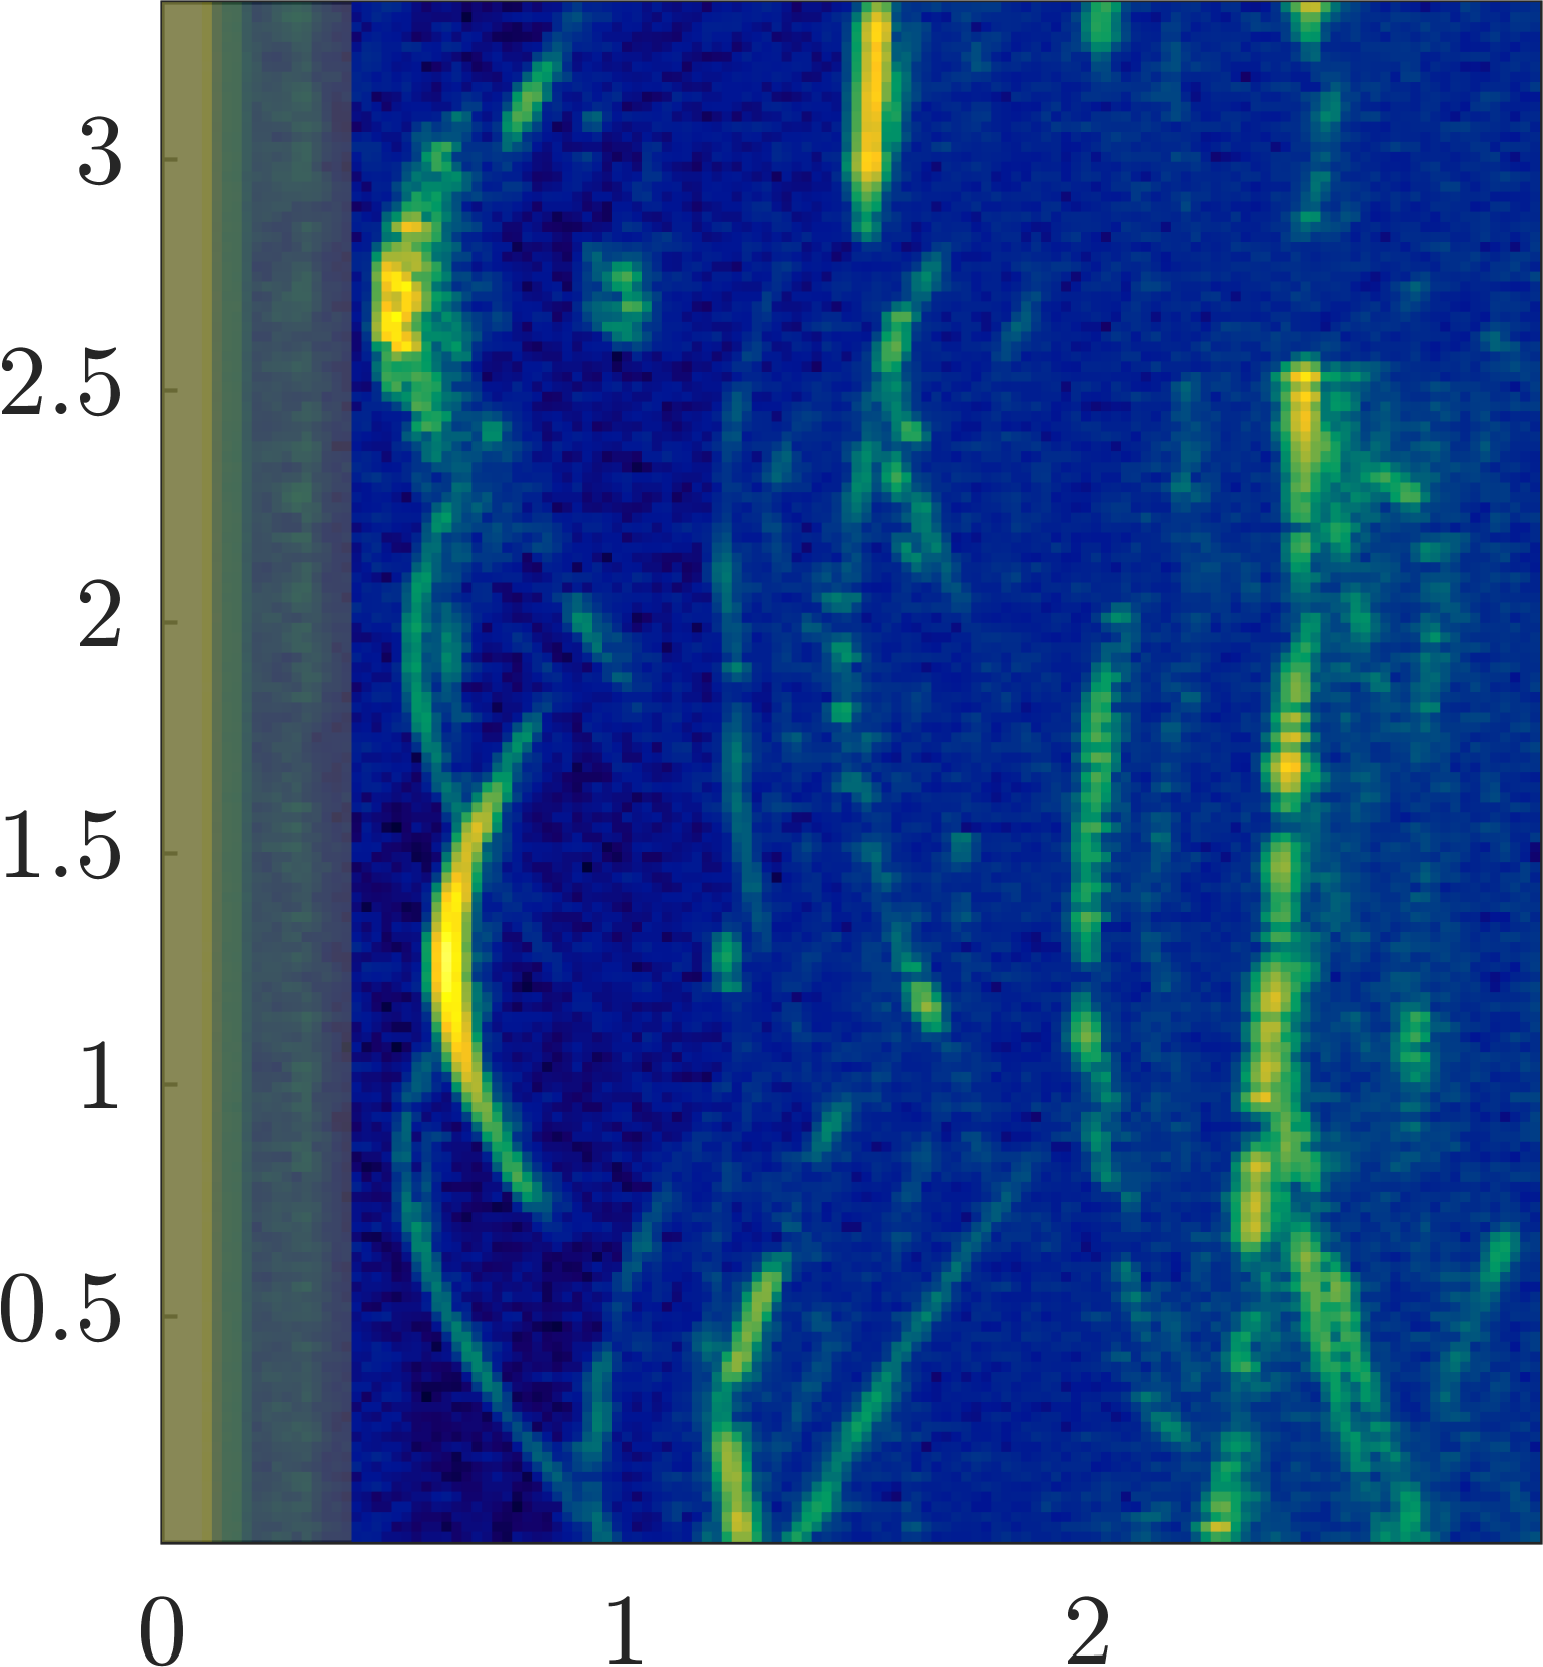
\includegraphics[width=\linewidth,max height=.475\textheight]{gfx/results/basement_input.png}
    \end{subfigure}%
    \hfill%
    \begin{subfigure}[t]{0.475\linewidth}  
        \centering 
        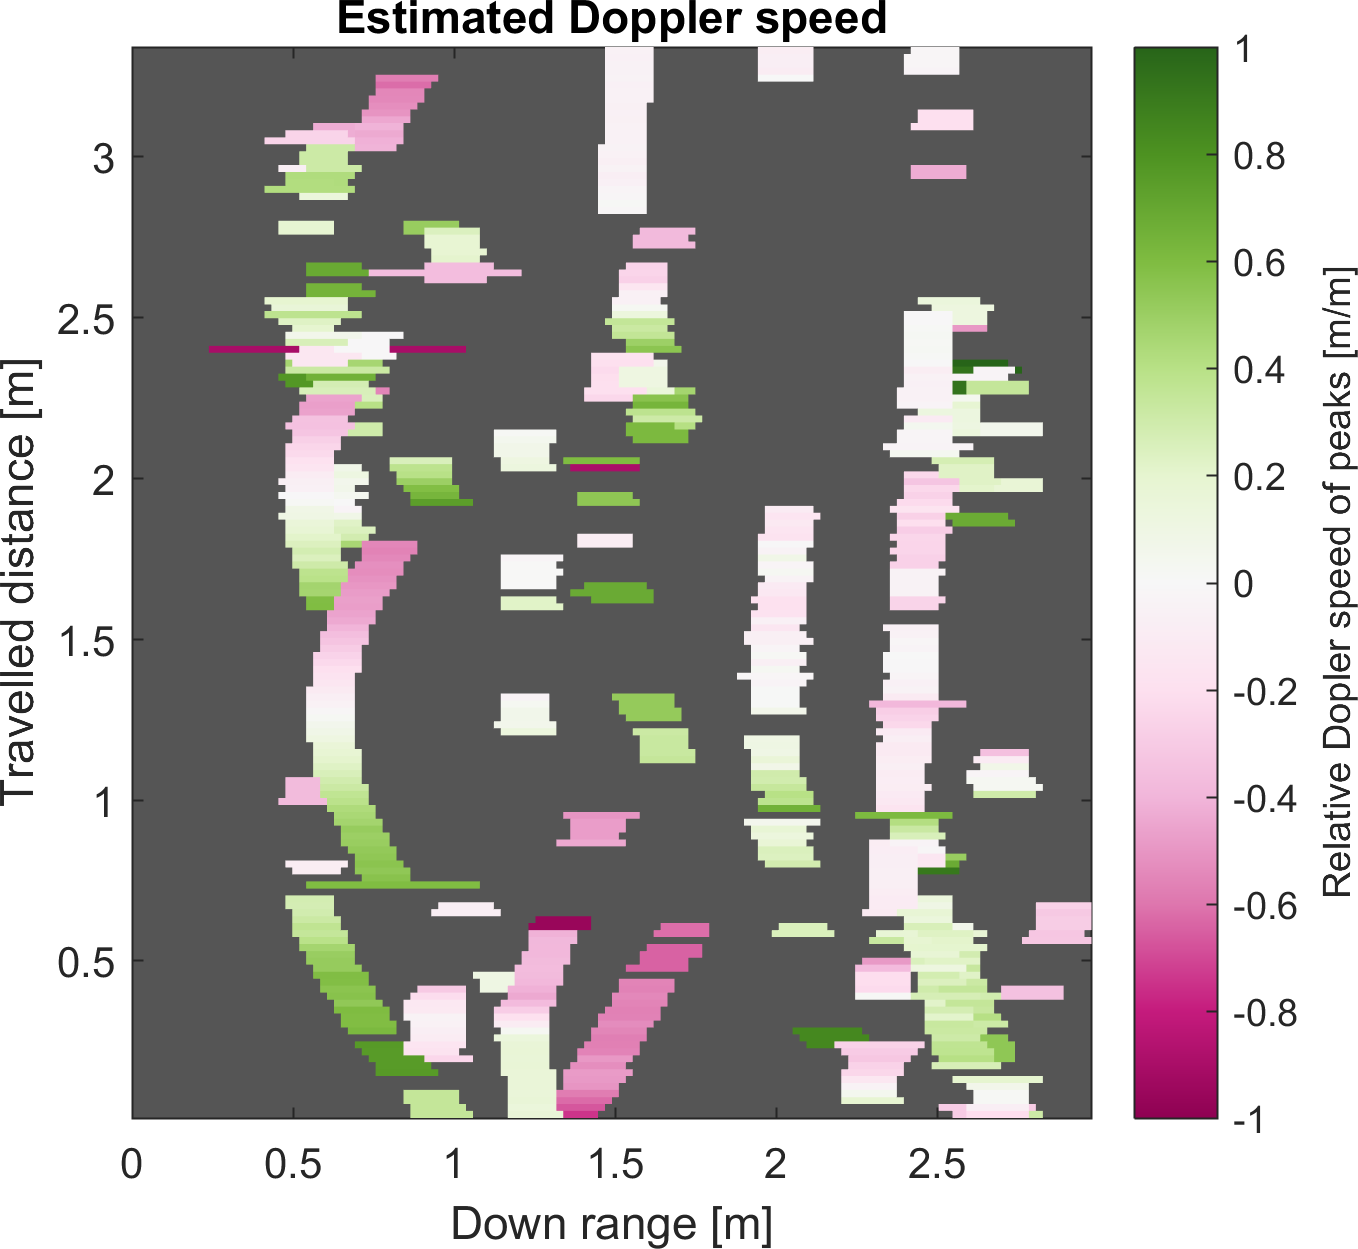
\includegraphics[width=\linewidth,max height=.475\textheight]{gfx/results/basement_doppler.png}
    \end{subfigure}\bigskip\\
    \begin{subfigure}[t]{0.5\linewidth}   
        \centering 
        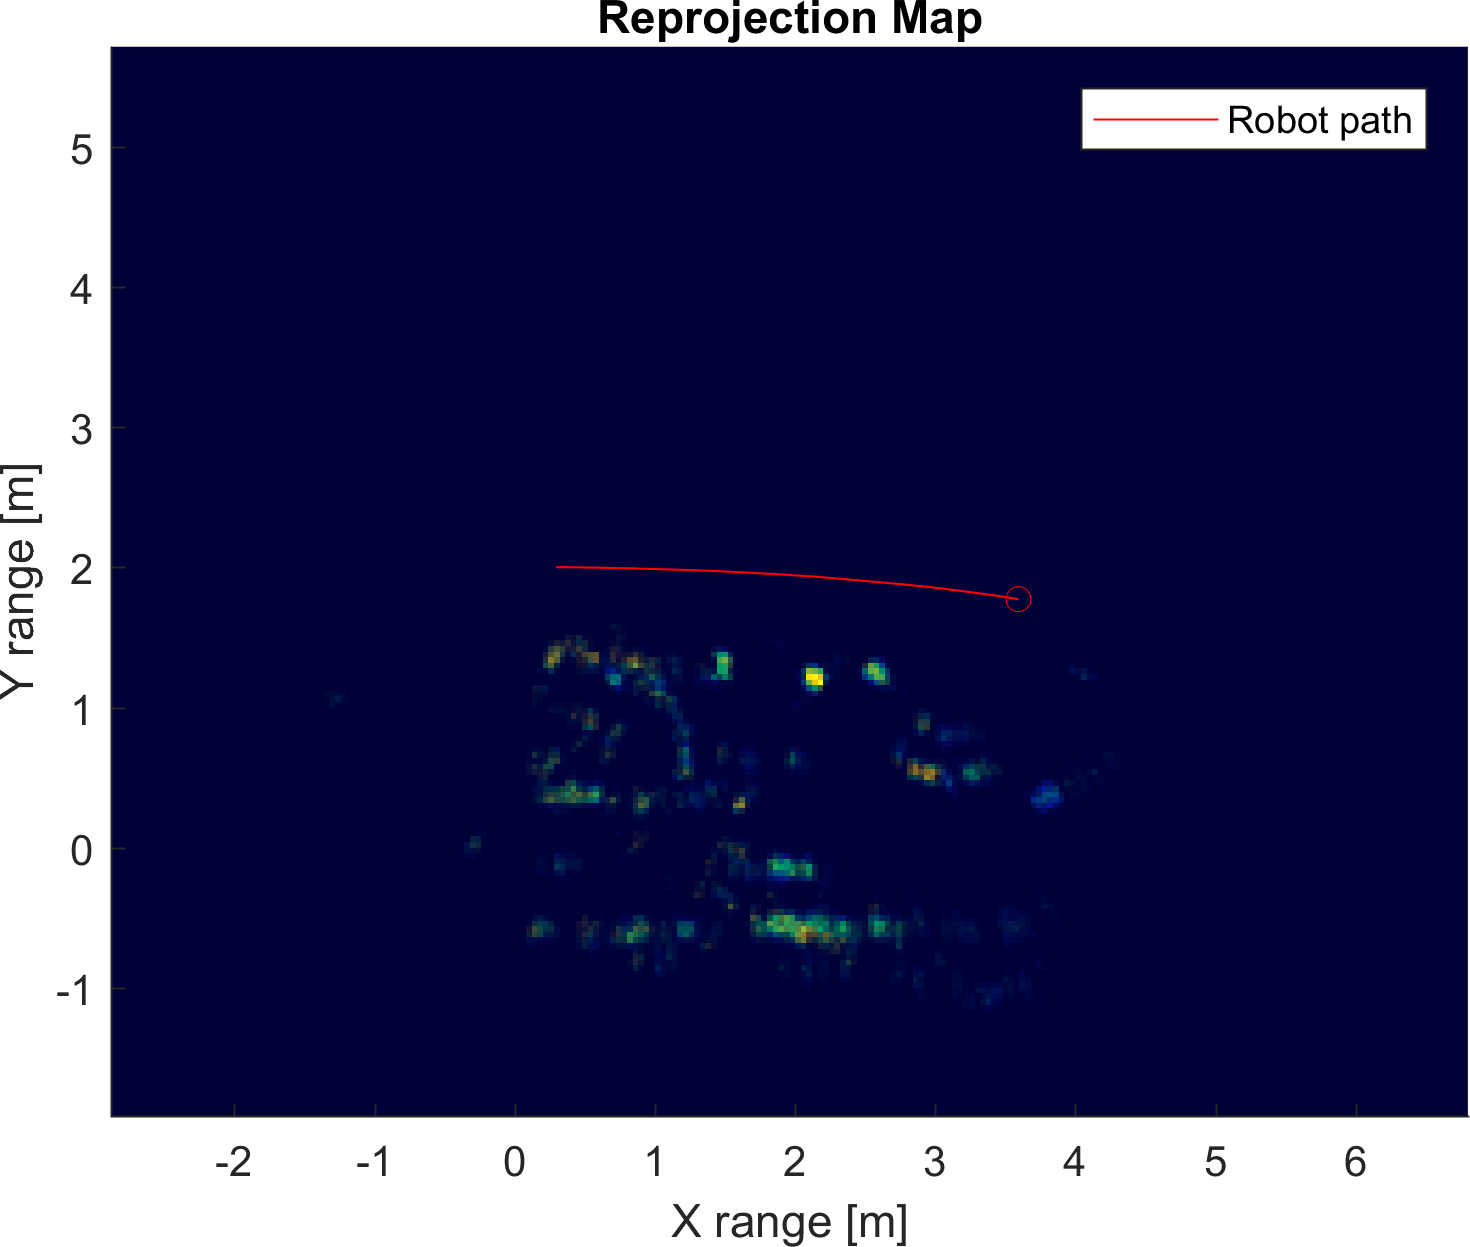
\includegraphics[width=\linewidth,max height=.475\textheight]{gfx/results/basement_reprojection.png}
    \end{subfigure}%
    \caption{Basement scan}
\end{figure}

\begin{figure}[htbp]
    \centering
    \begin{subfigure}[t]{0.475\linewidth}
        \centering
        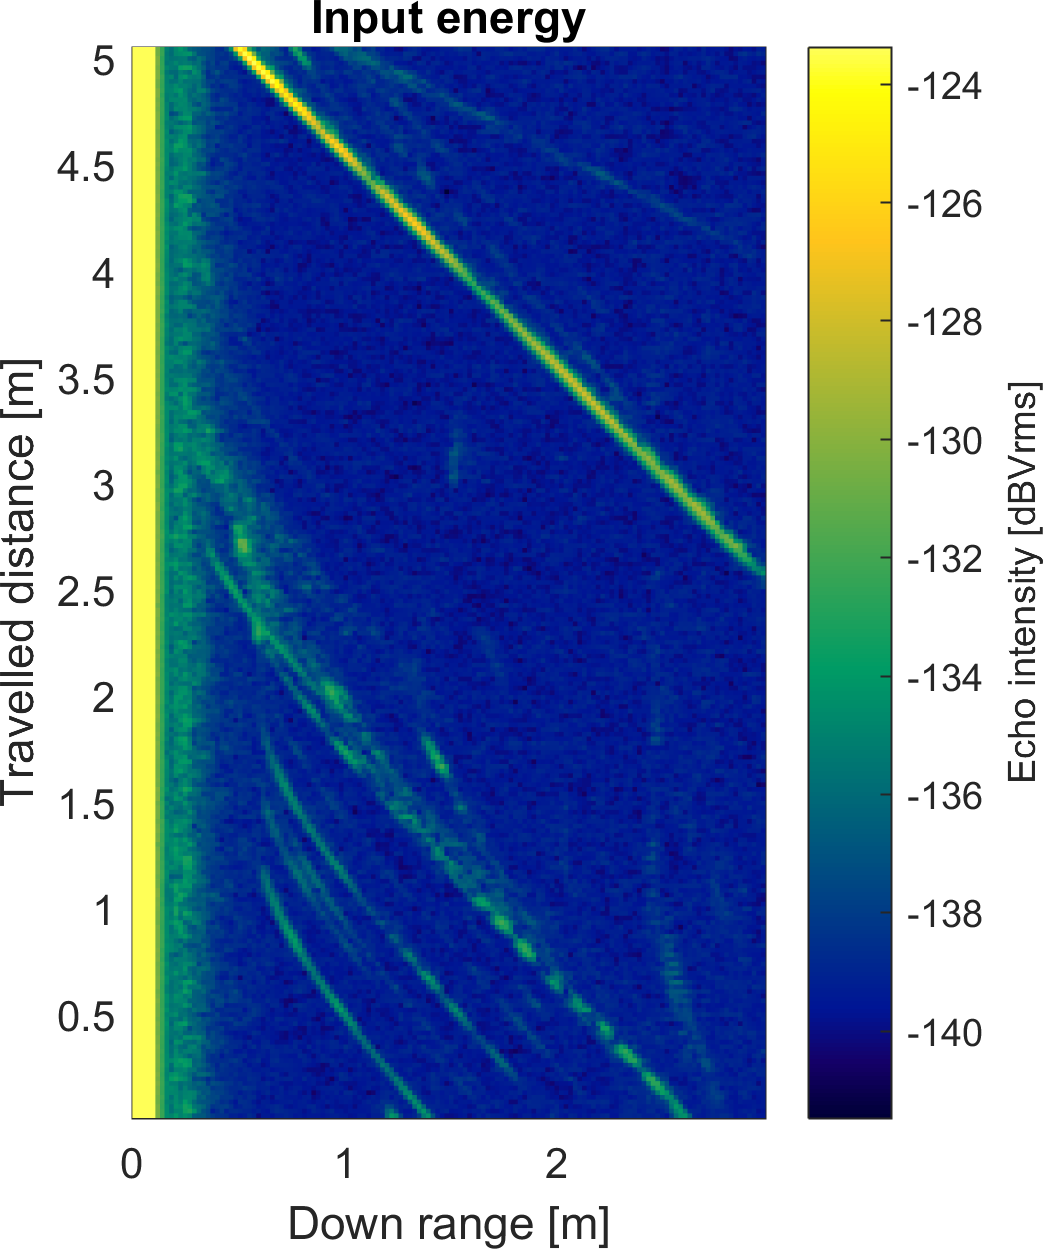
\includegraphics[width=\linewidth,max height=.475\textheight]{gfx/results/cafeteria_input.png}
    \end{subfigure}%
    \hfill%
    \begin{subfigure}[t]{0.475\linewidth}  
        \centering 
        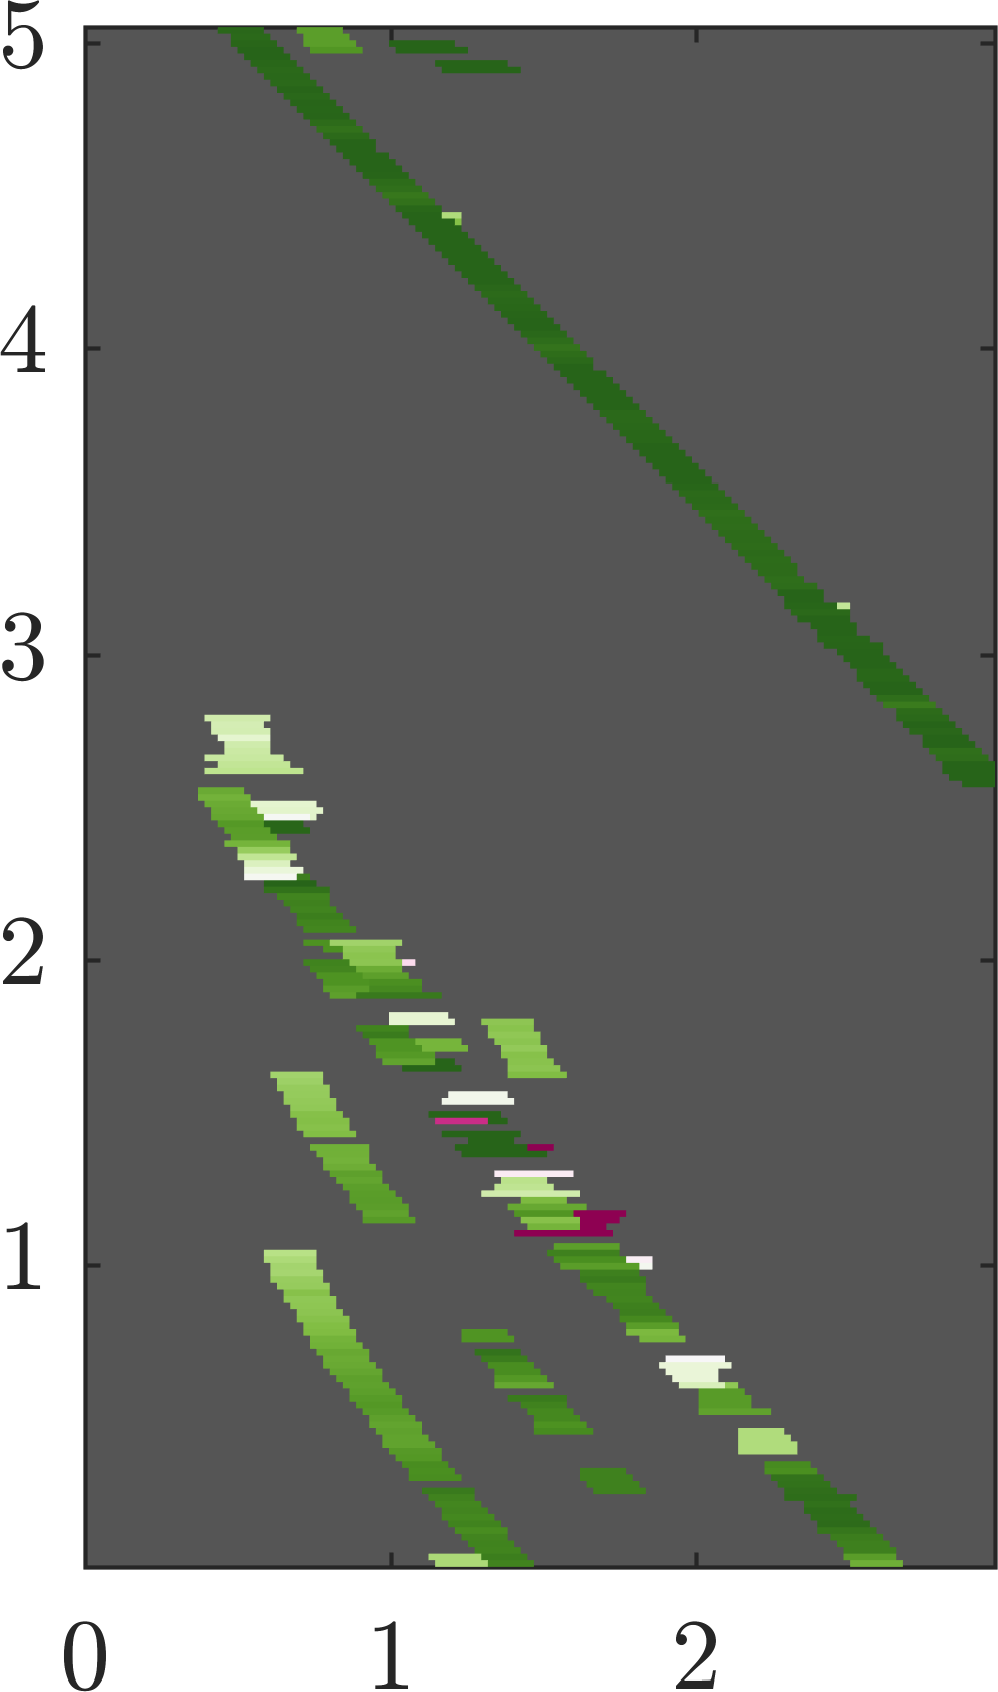
\includegraphics[width=\linewidth,max height=.475\textheight]{gfx/results/cafeteria_doppler.png}
    \end{subfigure}\bigskip\\
    \begin{subfigure}[t]{0.5\linewidth}   
        \centering 
        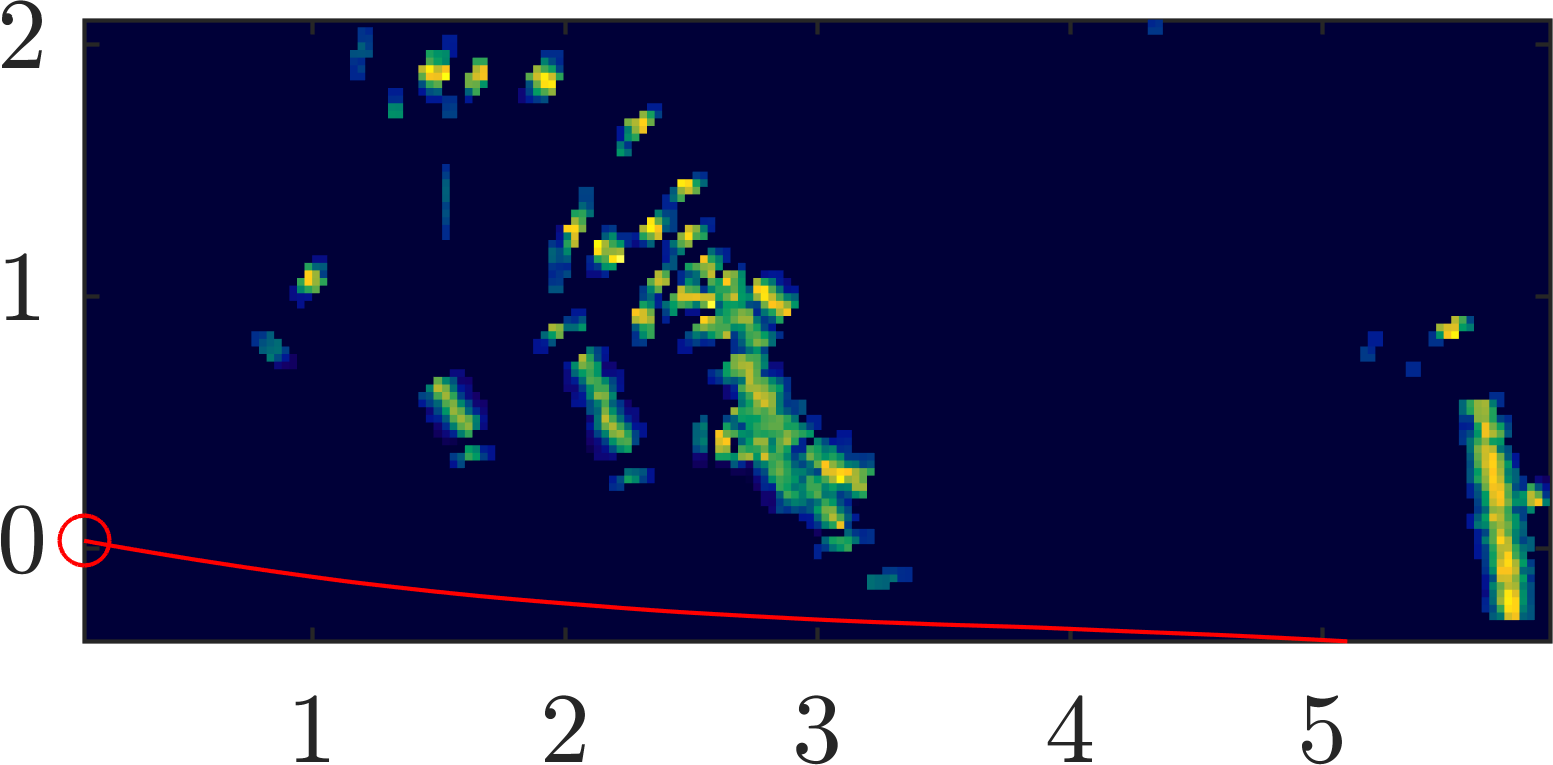
\includegraphics[width=\linewidth,max height=.475\textheight]{gfx/results/cafeteria_reprojection.png}
    \end{subfigure}%
    \caption{Cafeteria scan}
\end{figure}

\begin{figure}[htbp]
    \centering
    \begin{subfigure}[t]{0.475\linewidth}
        \centering
        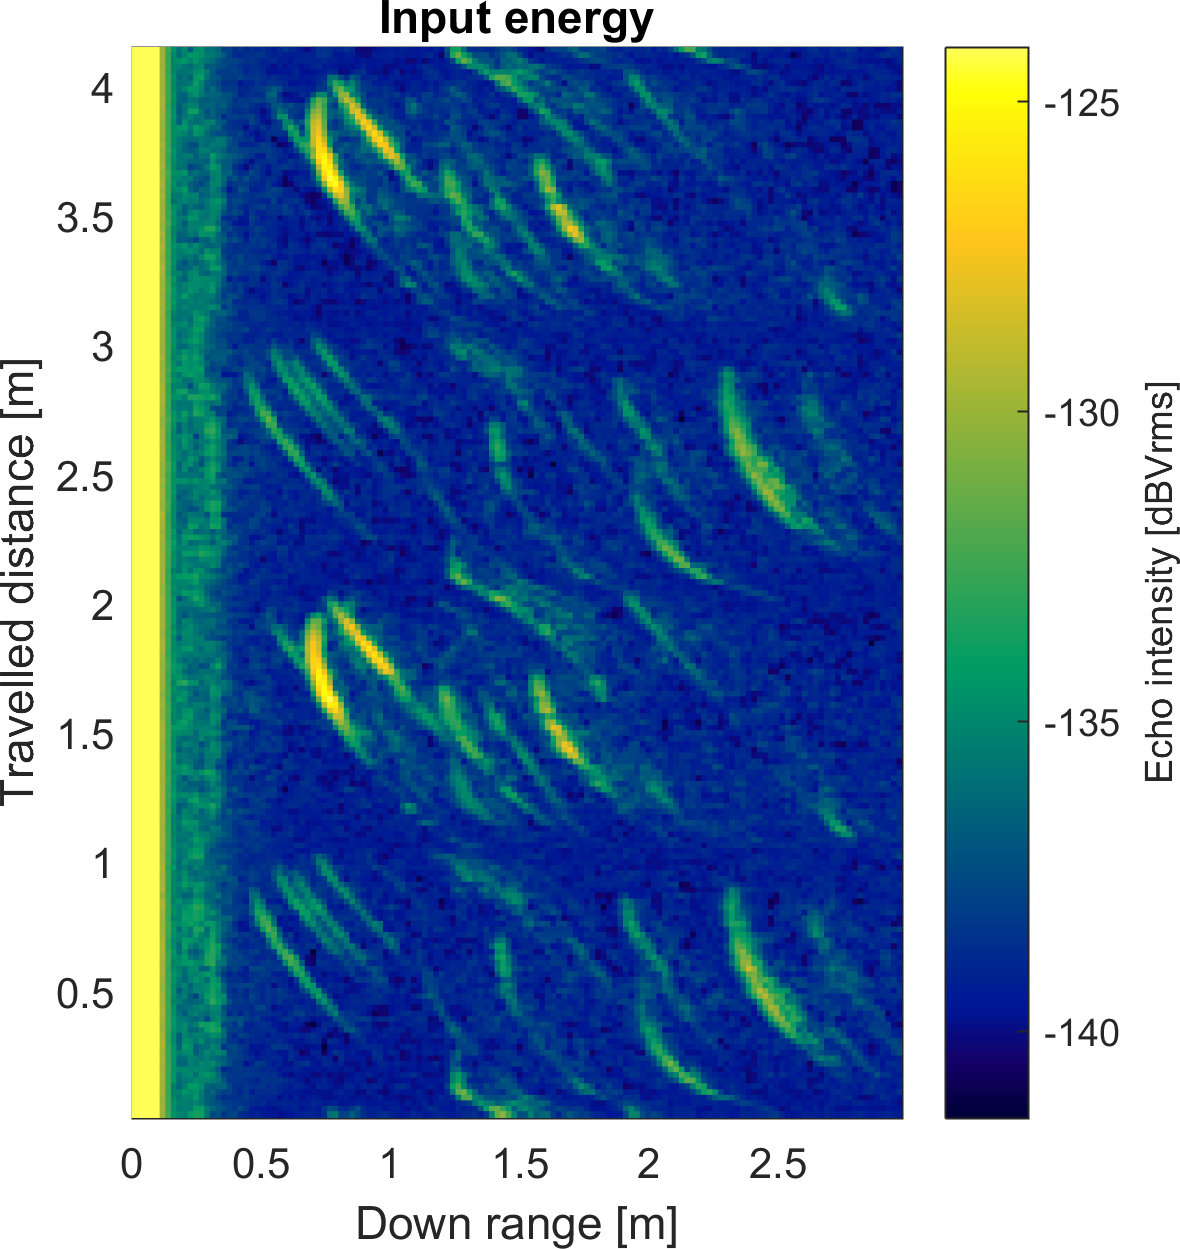
\includegraphics[width=\linewidth,max height=.475\textheight]{gfx/results/dungeon_input.png}
    \end{subfigure}%
    \hfill%
    \begin{subfigure}[t]{0.475\linewidth}  
        \centering 
        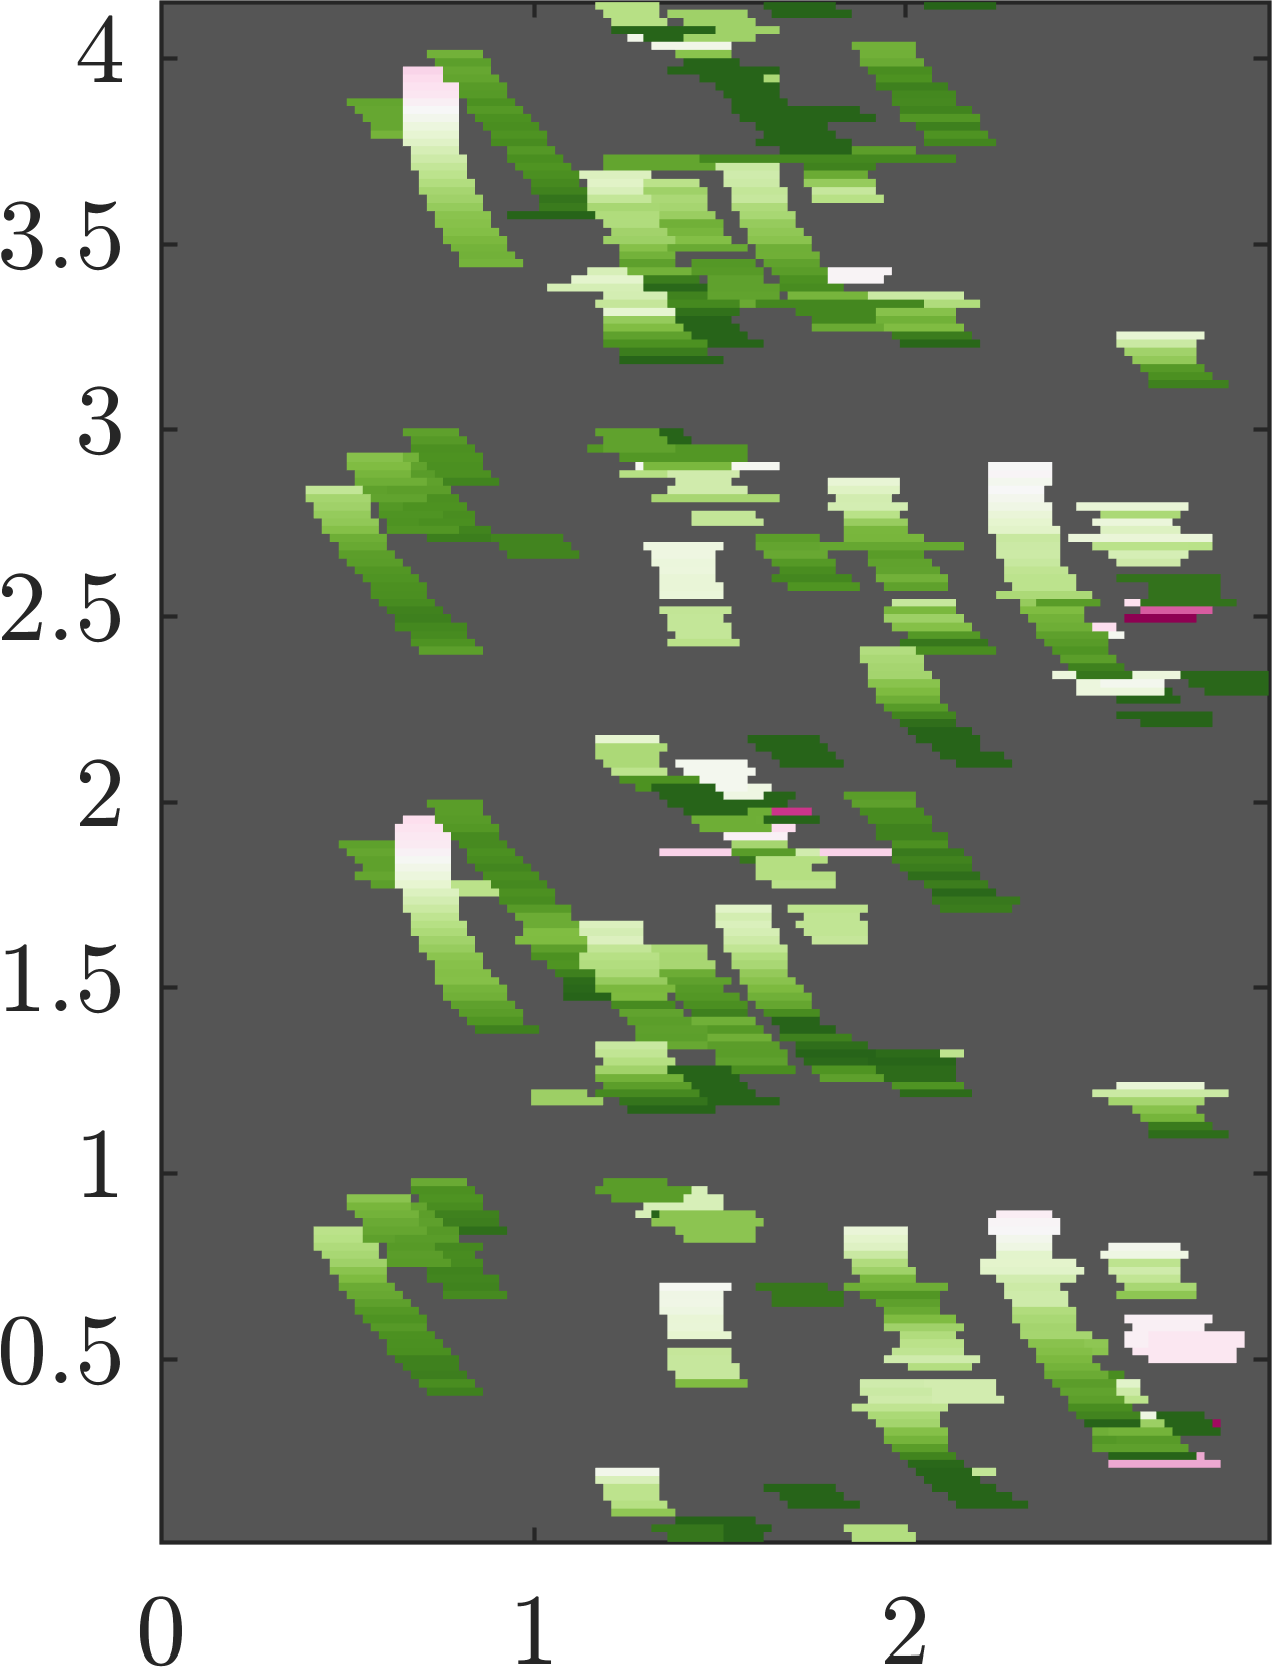
\includegraphics[width=\linewidth,max height=.475\textheight]{gfx/results/dungeon_doppler.png}
    \end{subfigure}\bigskip\\
    \begin{subfigure}[t]{0.5\linewidth}   
        \centering 
        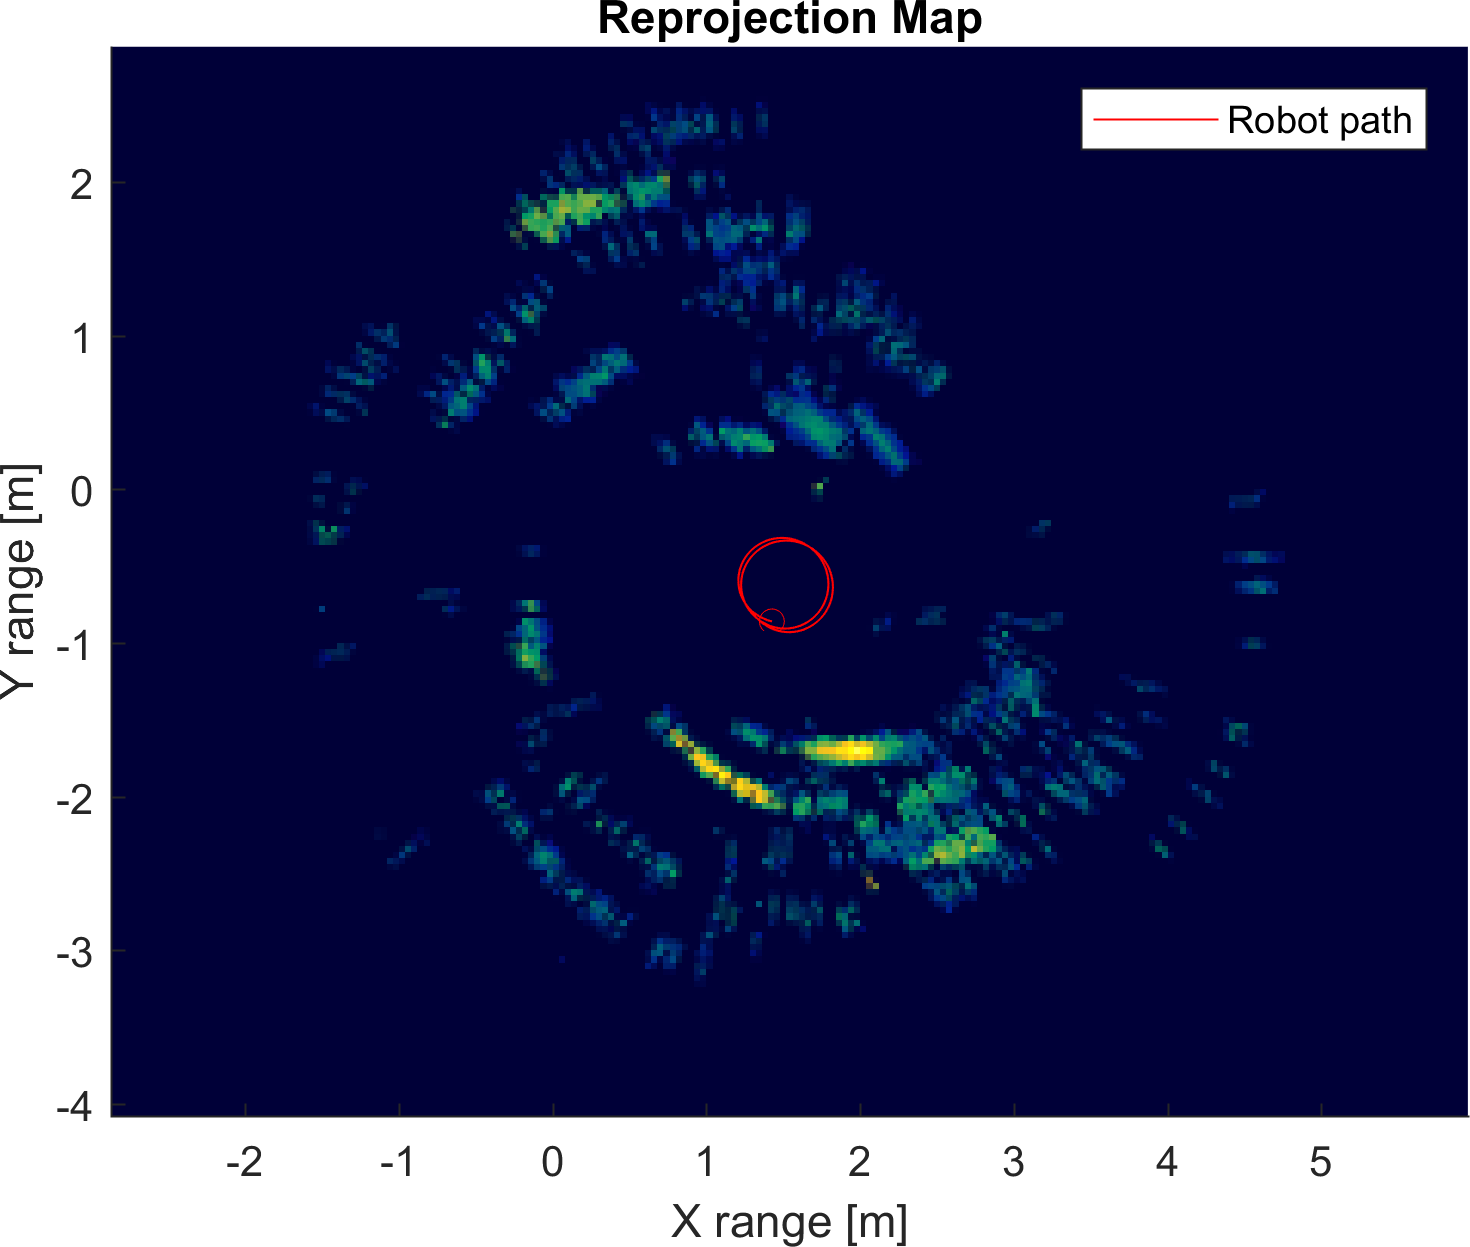
\includegraphics[width=\linewidth,max height=.475\textheight]{gfx/results/dungeon_reprojection.png}
    \end{subfigure}%
    \caption{Dungeon scan}
\end{figure}

\begin{figure}[htbp]
    \centering
    \begin{subfigure}[t]{0.475\linewidth}
        \centering
        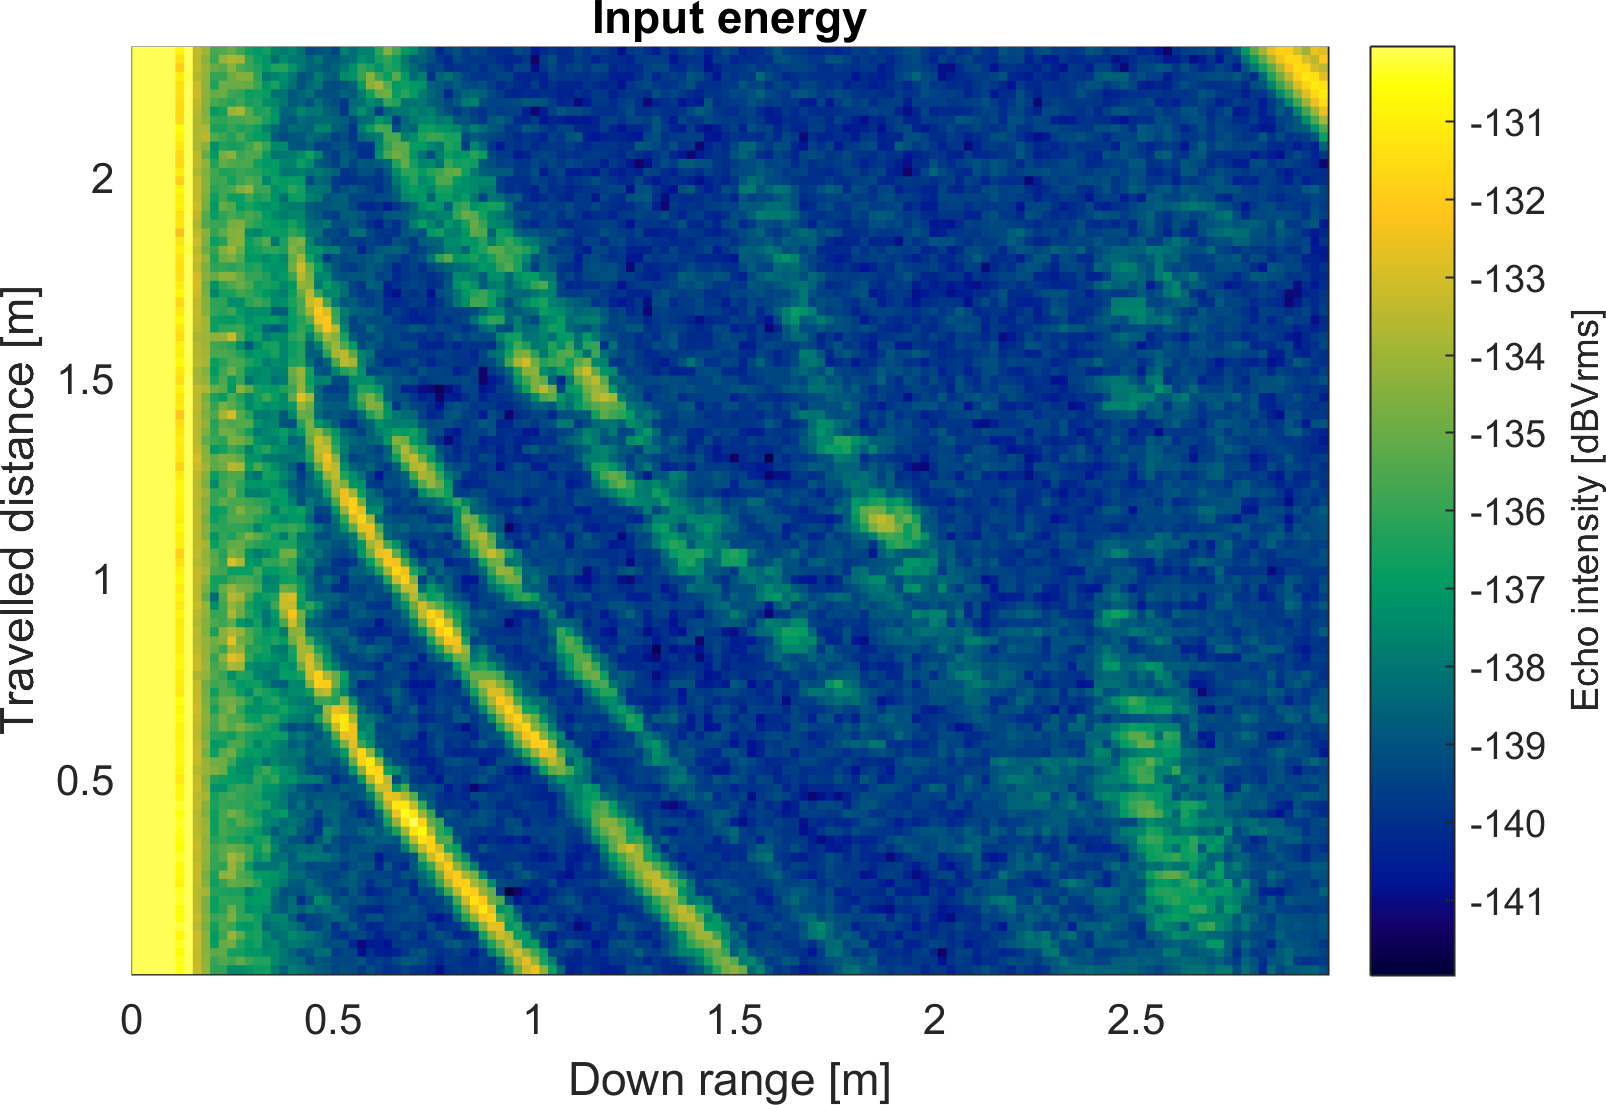
\includegraphics[width=\linewidth,max height=.475\textheight]{gfx/results/entryway_input.png}
    \end{subfigure}%
    \hfill%
    \begin{subfigure}[t]{0.475\linewidth}  
        \centering 
        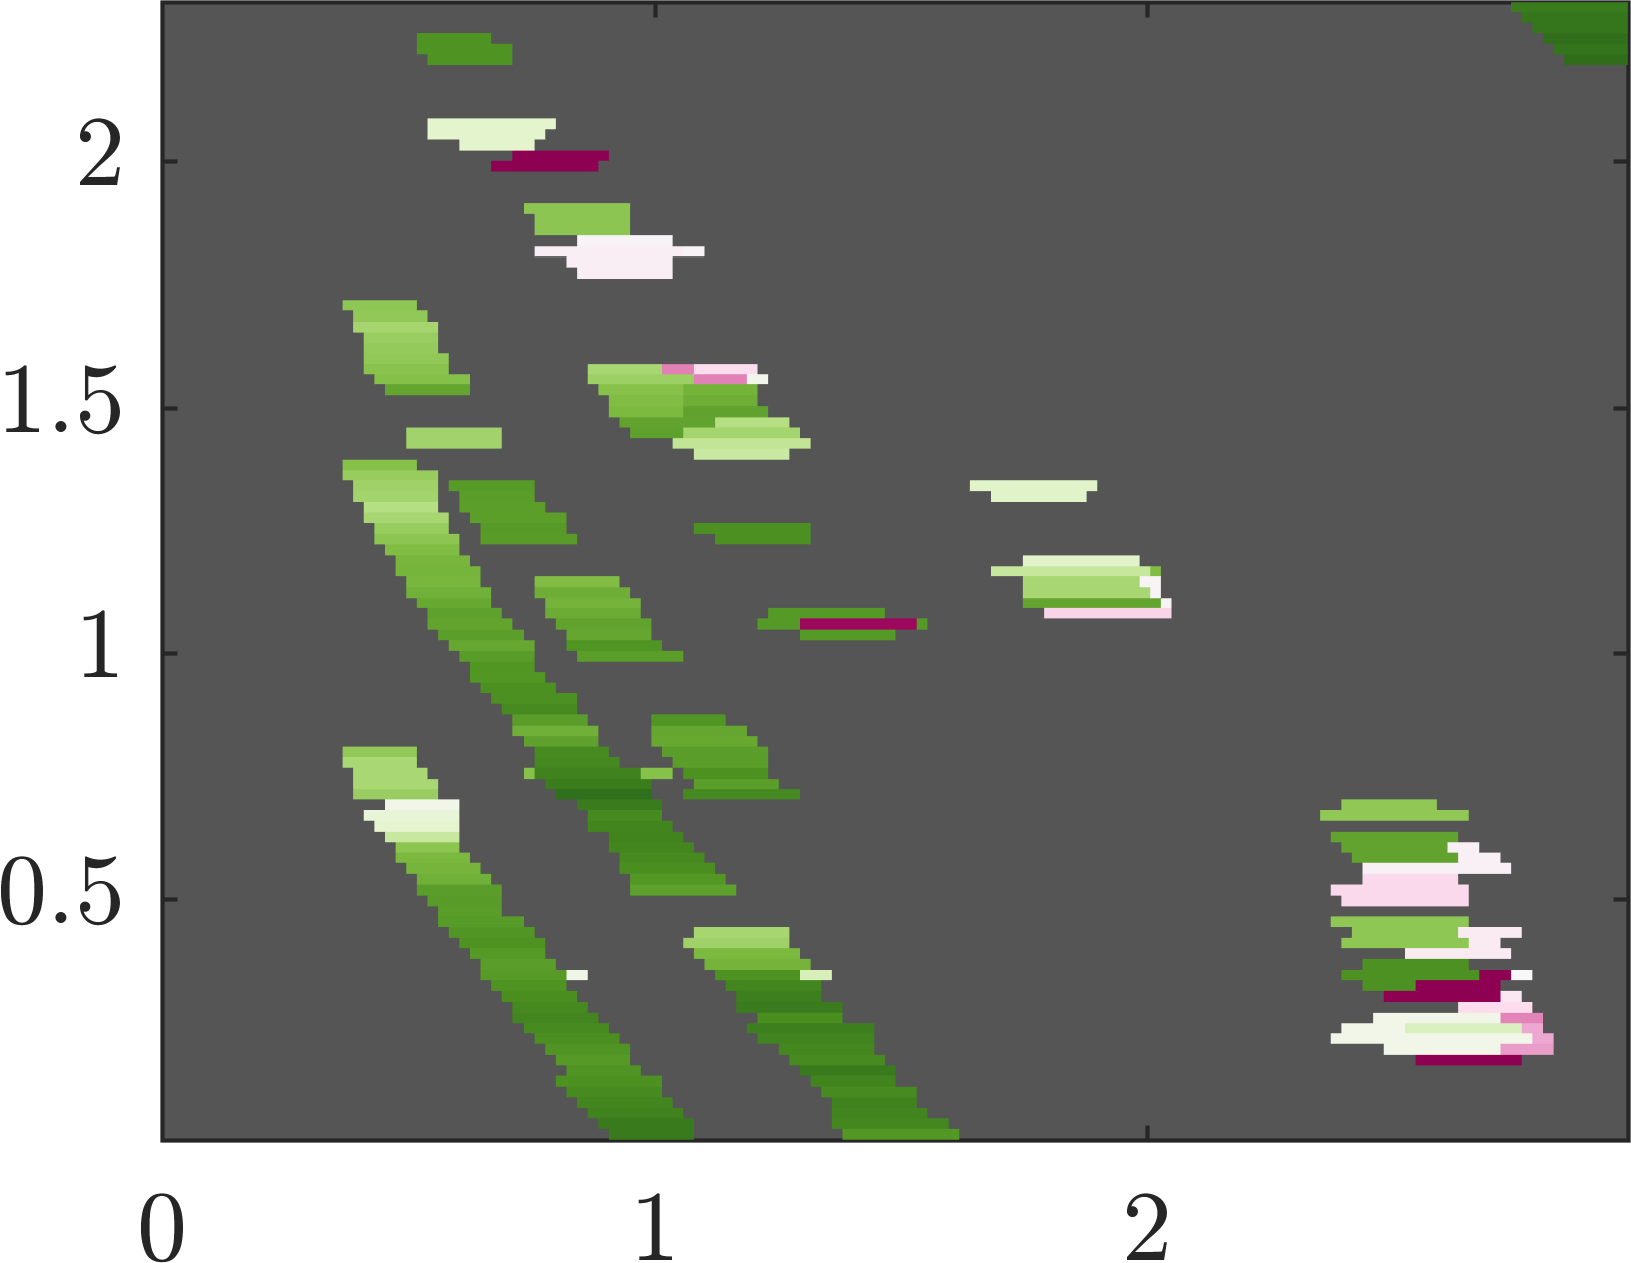
\includegraphics[width=\linewidth,max height=.475\textheight]{gfx/results/entryway_doppler.png}
    \end{subfigure}\bigskip\\
    \begin{subfigure}[t]{0.5\linewidth}   
        \centering 
        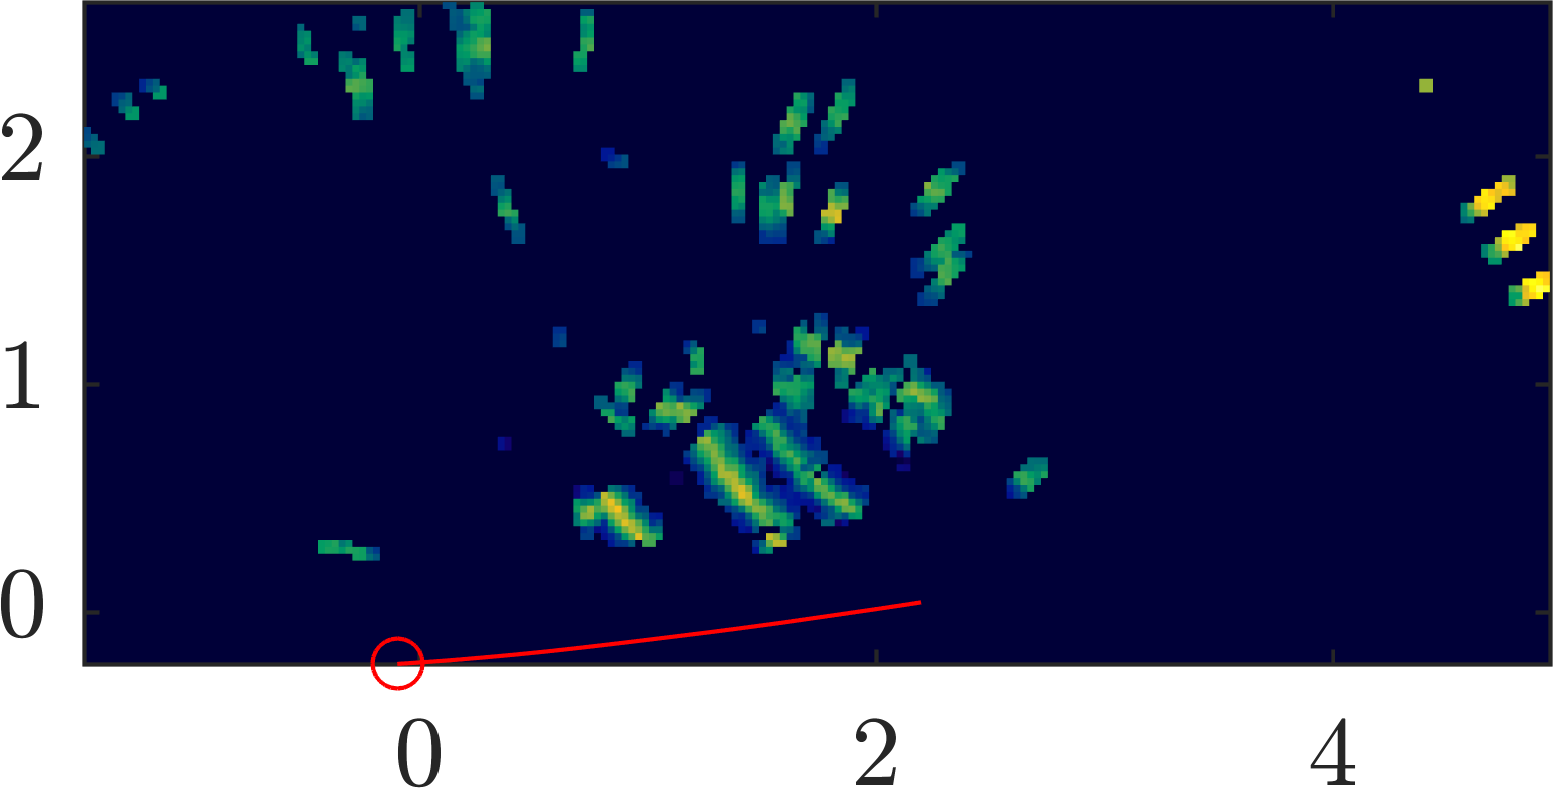
\includegraphics[width=\linewidth,max height=.475\textheight]{gfx/results/entryway_reprojection.png}
    \end{subfigure}%
    \caption{Entryway scan}
\end{figure}

\begin{figure}[htbp]
    \centering
    \begin{subfigure}[t]{0.475\linewidth}
        \centering
        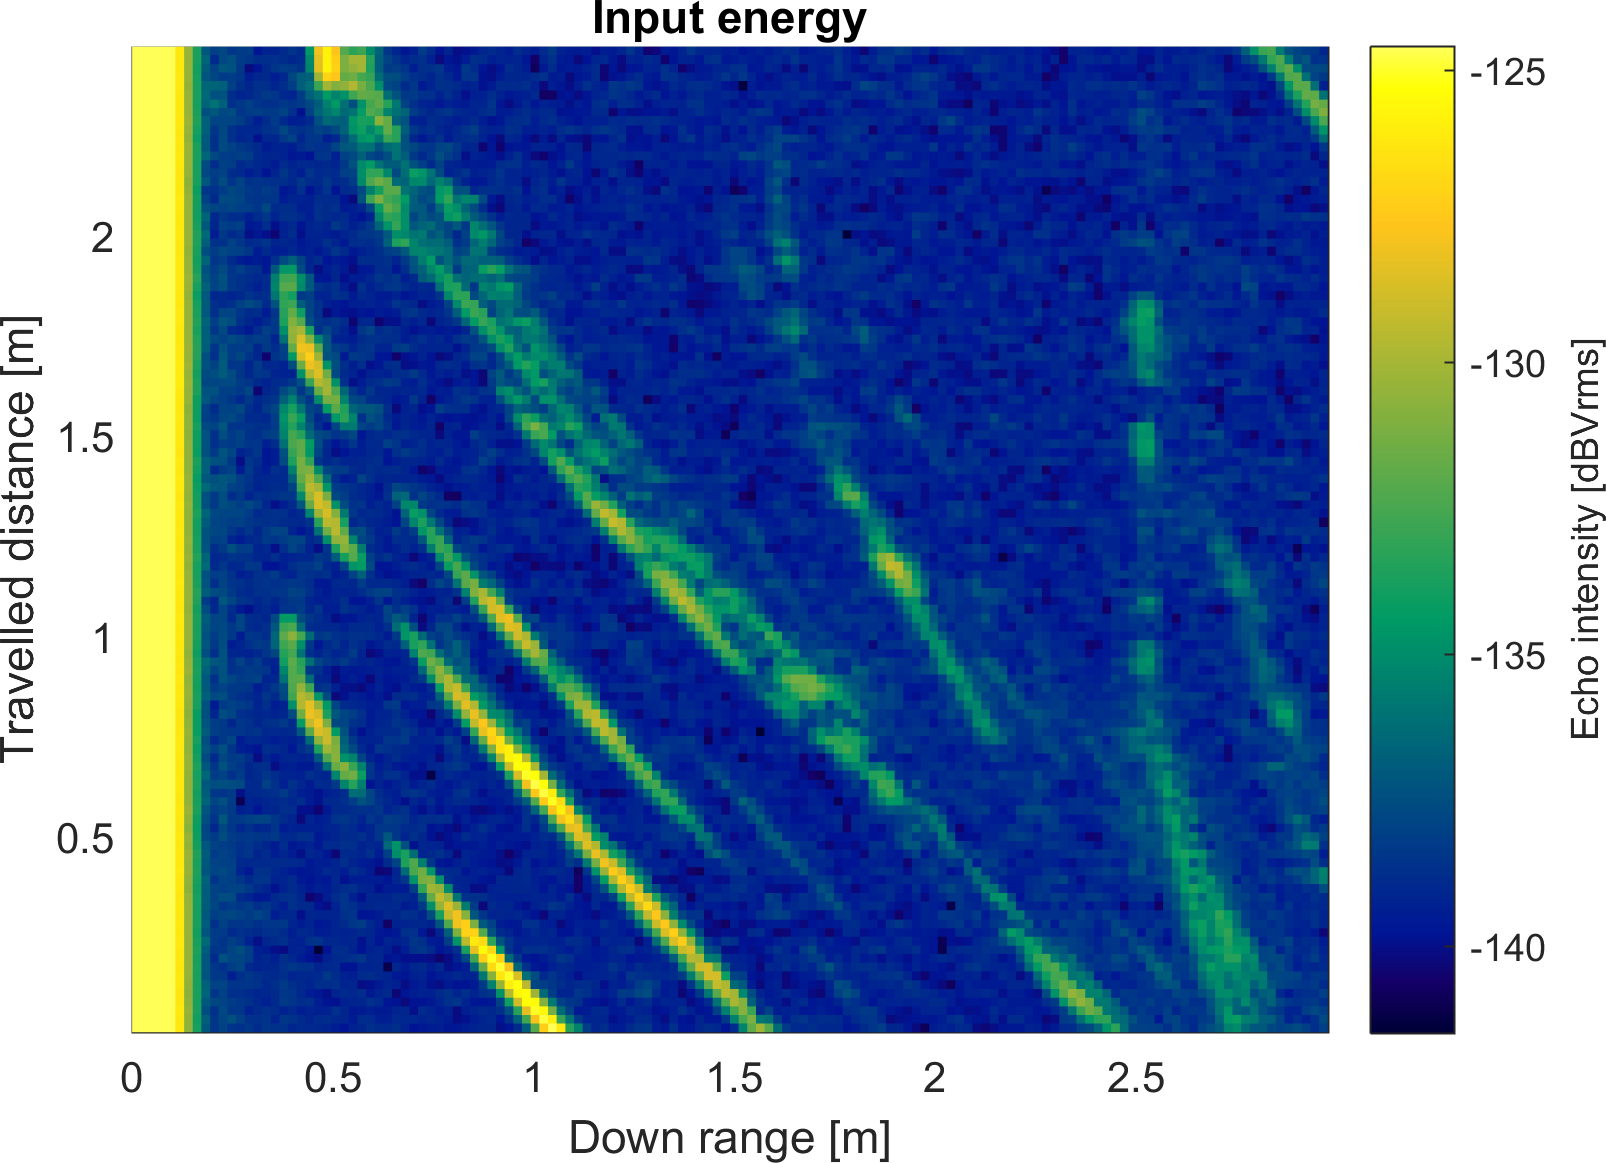
\includegraphics[width=\linewidth,max height=.475\textheight]{gfx/results/falloutshelter_input.png}
    \end{subfigure}%
    \hfill%
    \begin{subfigure}[t]{0.475\linewidth}  
        \centering 
        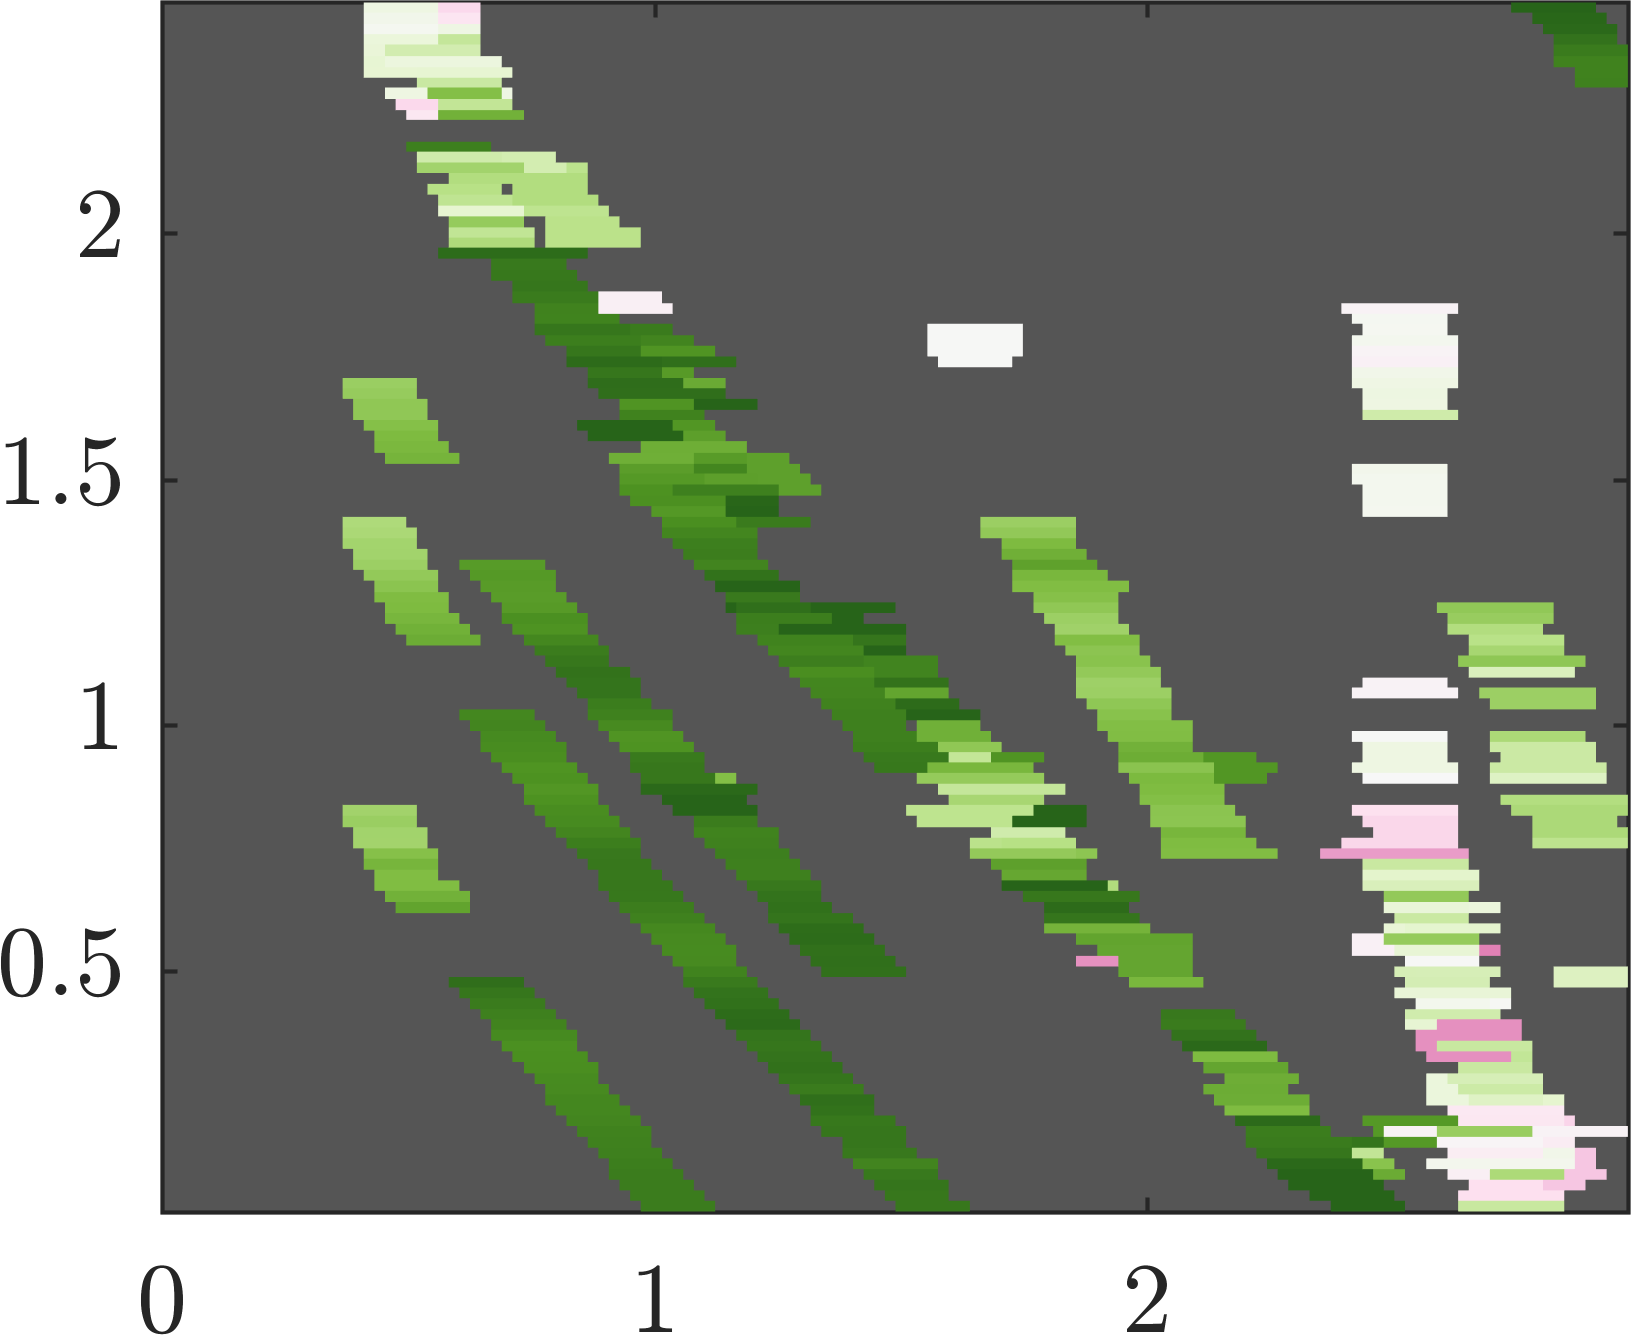
\includegraphics[width=\linewidth,max height=.475\textheight]{gfx/results/falloutshelter_doppler.png}
    \end{subfigure}\bigskip\\
    \begin{subfigure}[t]{0.5\linewidth}   
        \centering 
        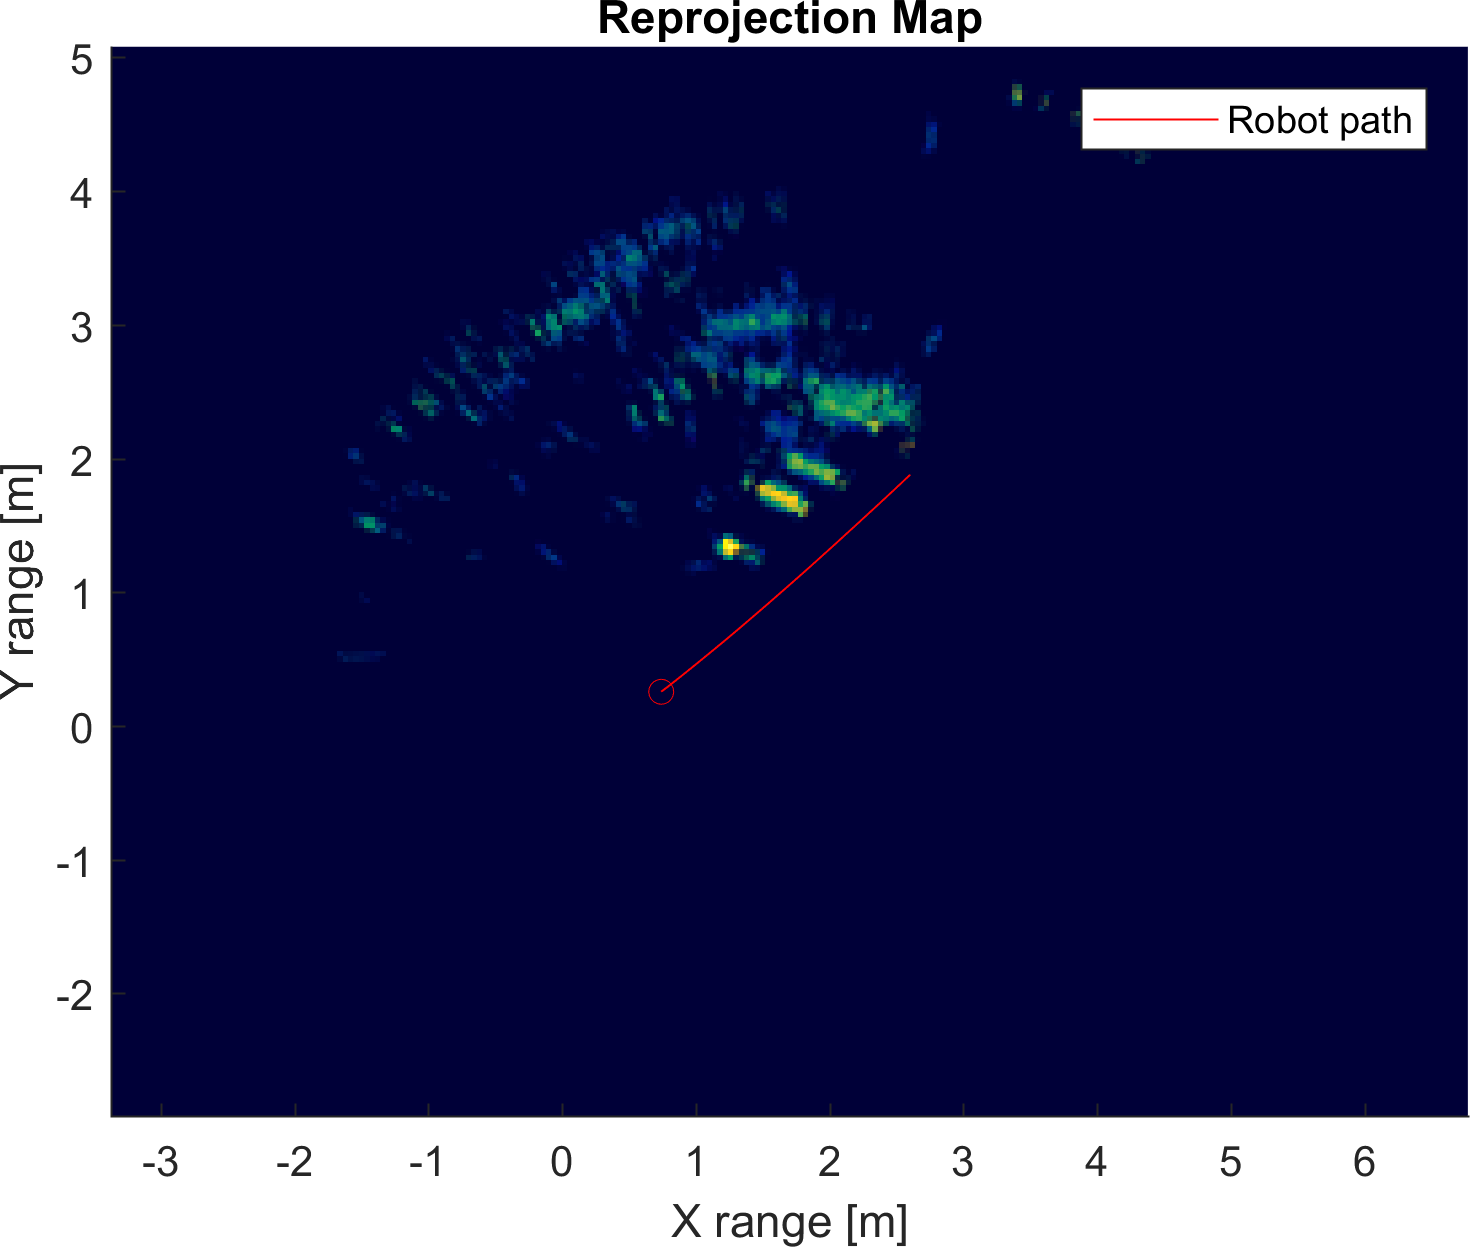
\includegraphics[width=\linewidth,max height=.475\textheight]{gfx/results/falloutshelter_reprojection.png}
    \end{subfigure}%
    \caption{Fallout Shelter scan}
\end{figure}

\begin{figure}[htbp]
    \centering
    \begin{subfigure}[t]{0.475\linewidth}
        \centering
        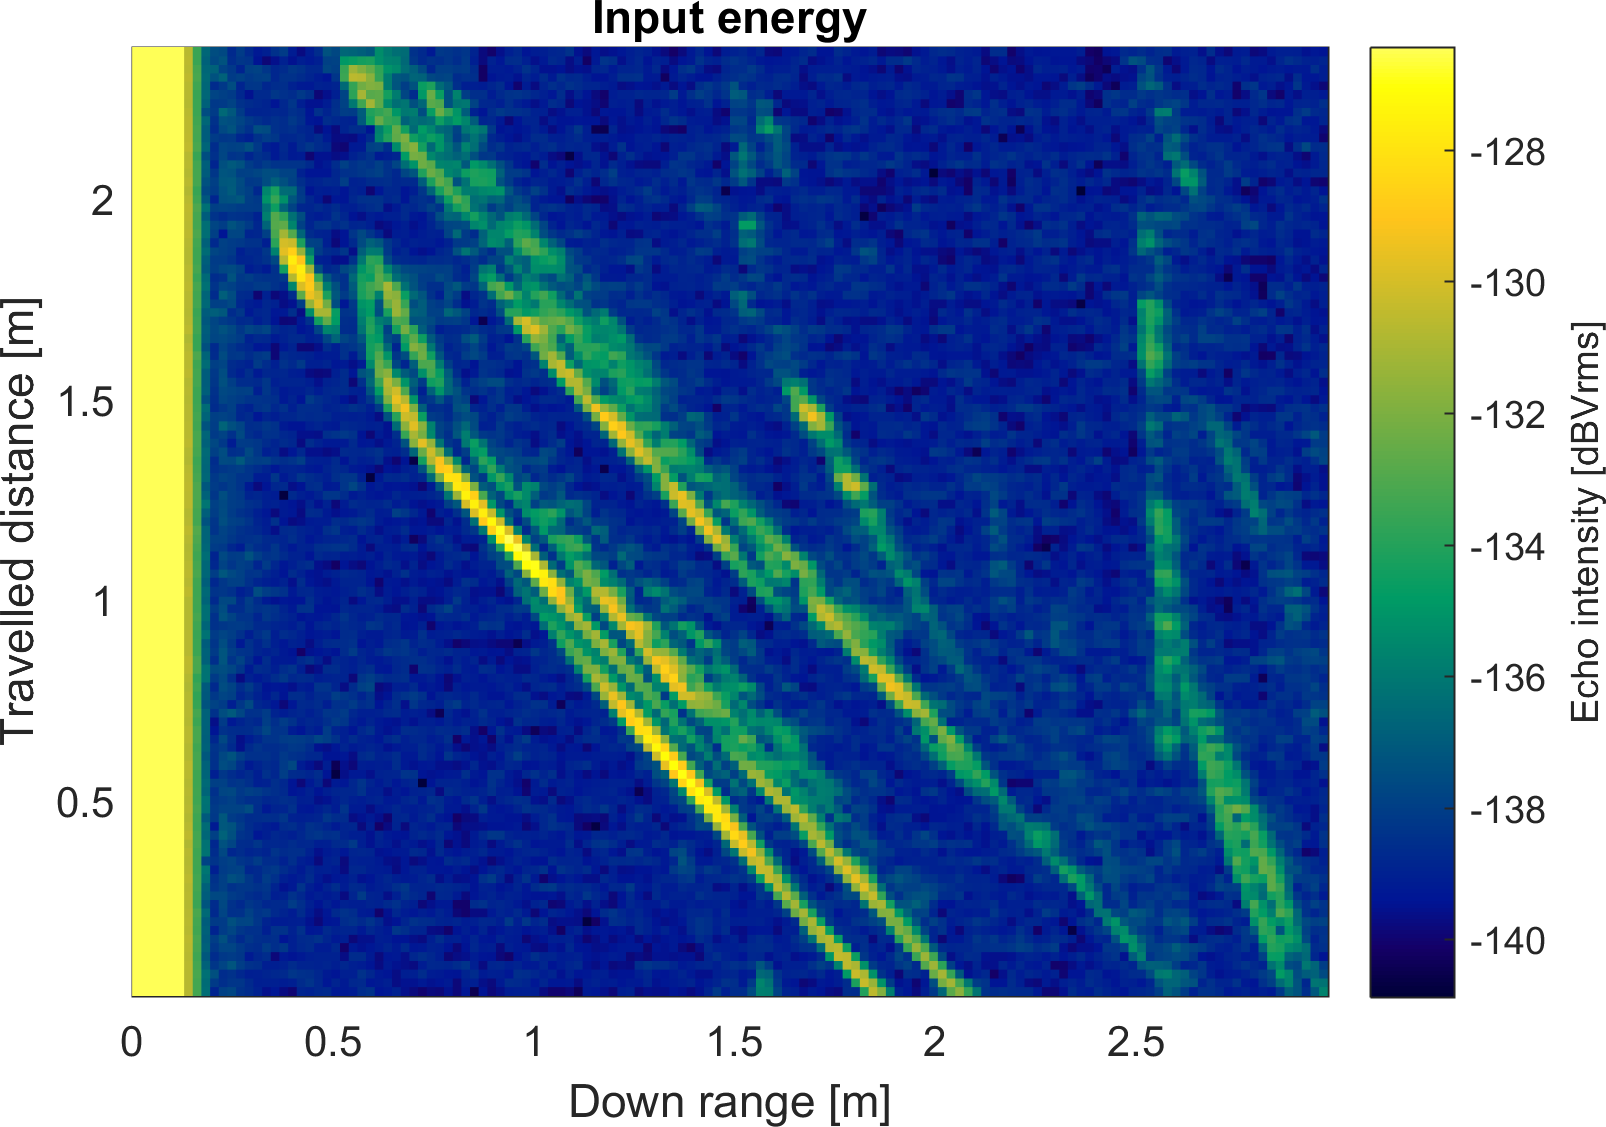
\includegraphics[width=\linewidth,max height=.475\textheight]{gfx/results/garden_input.png}
    \end{subfigure}%
    \hfill%
    \begin{subfigure}[t]{0.475\linewidth}  
        \centering 
        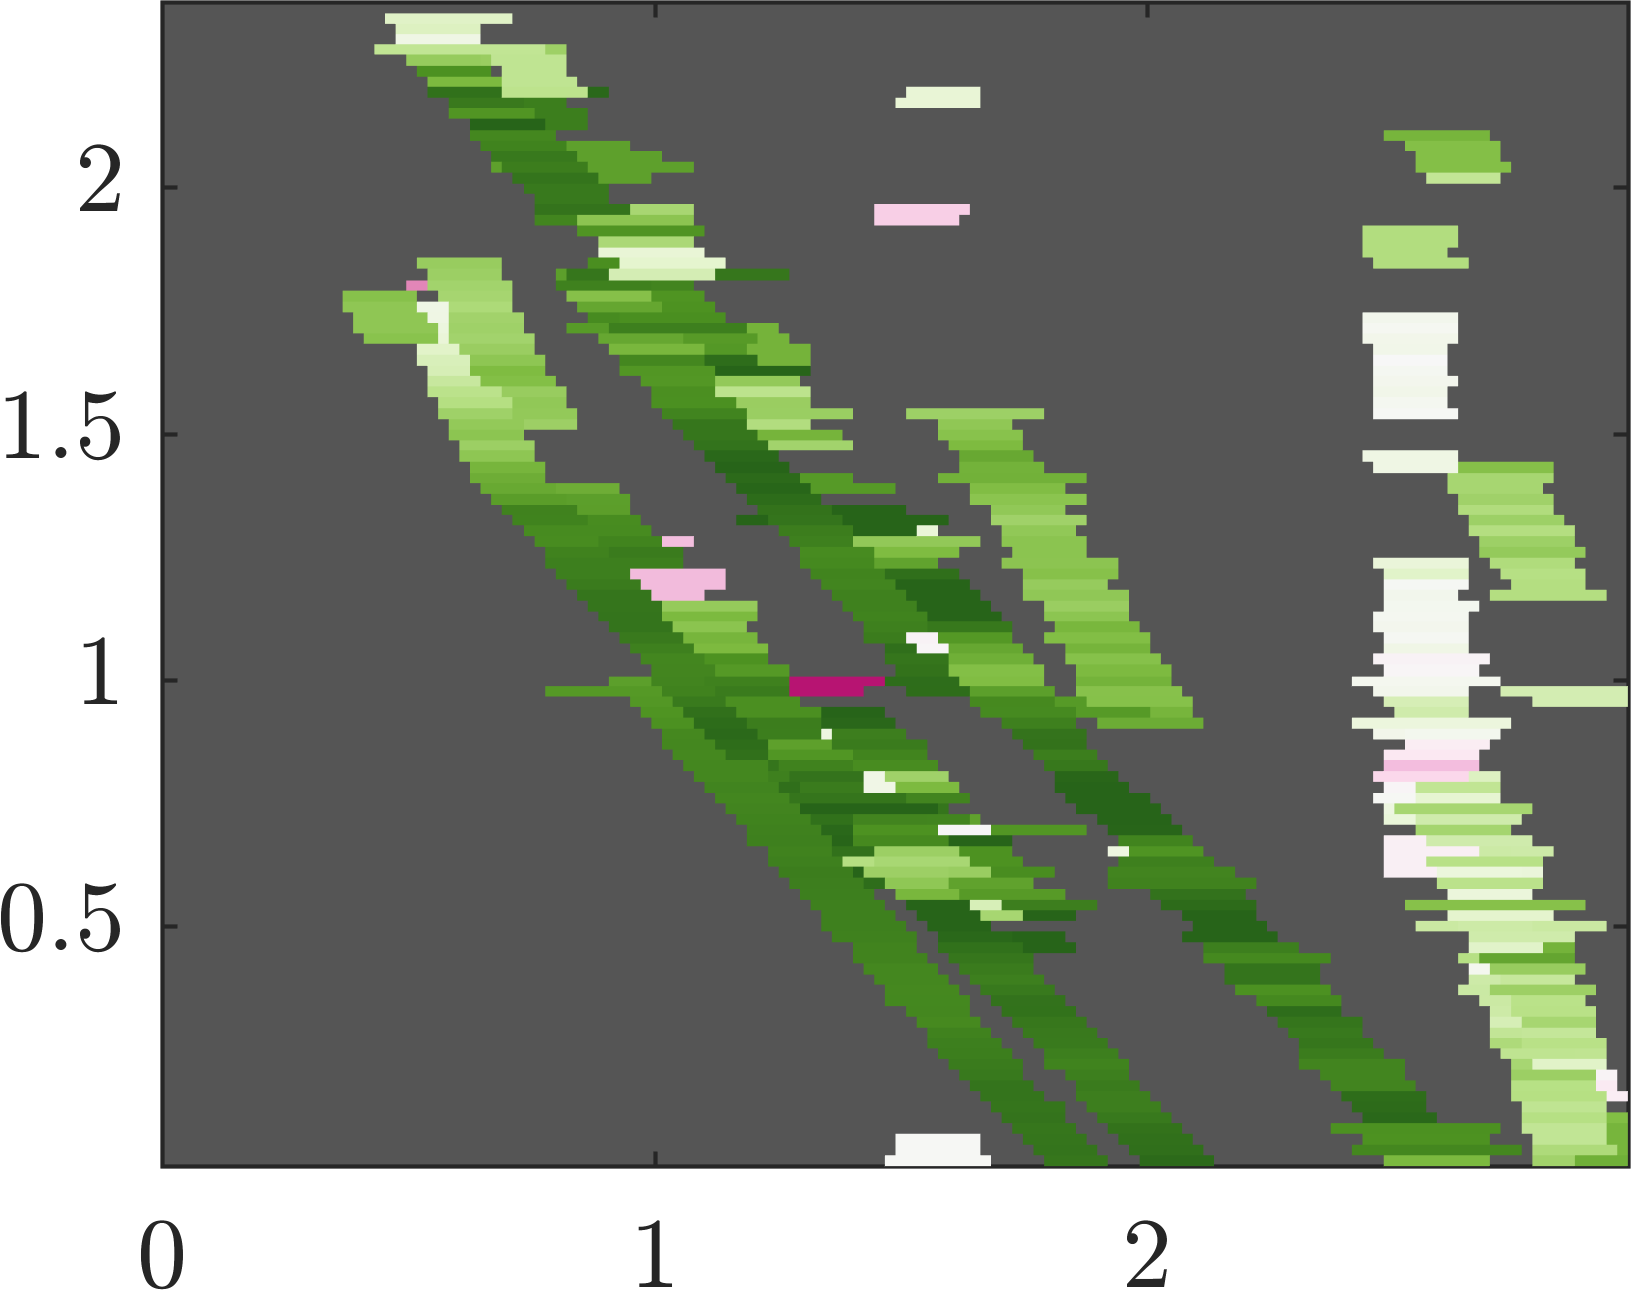
\includegraphics[width=\linewidth,max height=.475\textheight]{gfx/results/garden_doppler.png}
    \end{subfigure}\bigskip\\
    \begin{subfigure}[t]{0.5\linewidth}   
        \centering 
        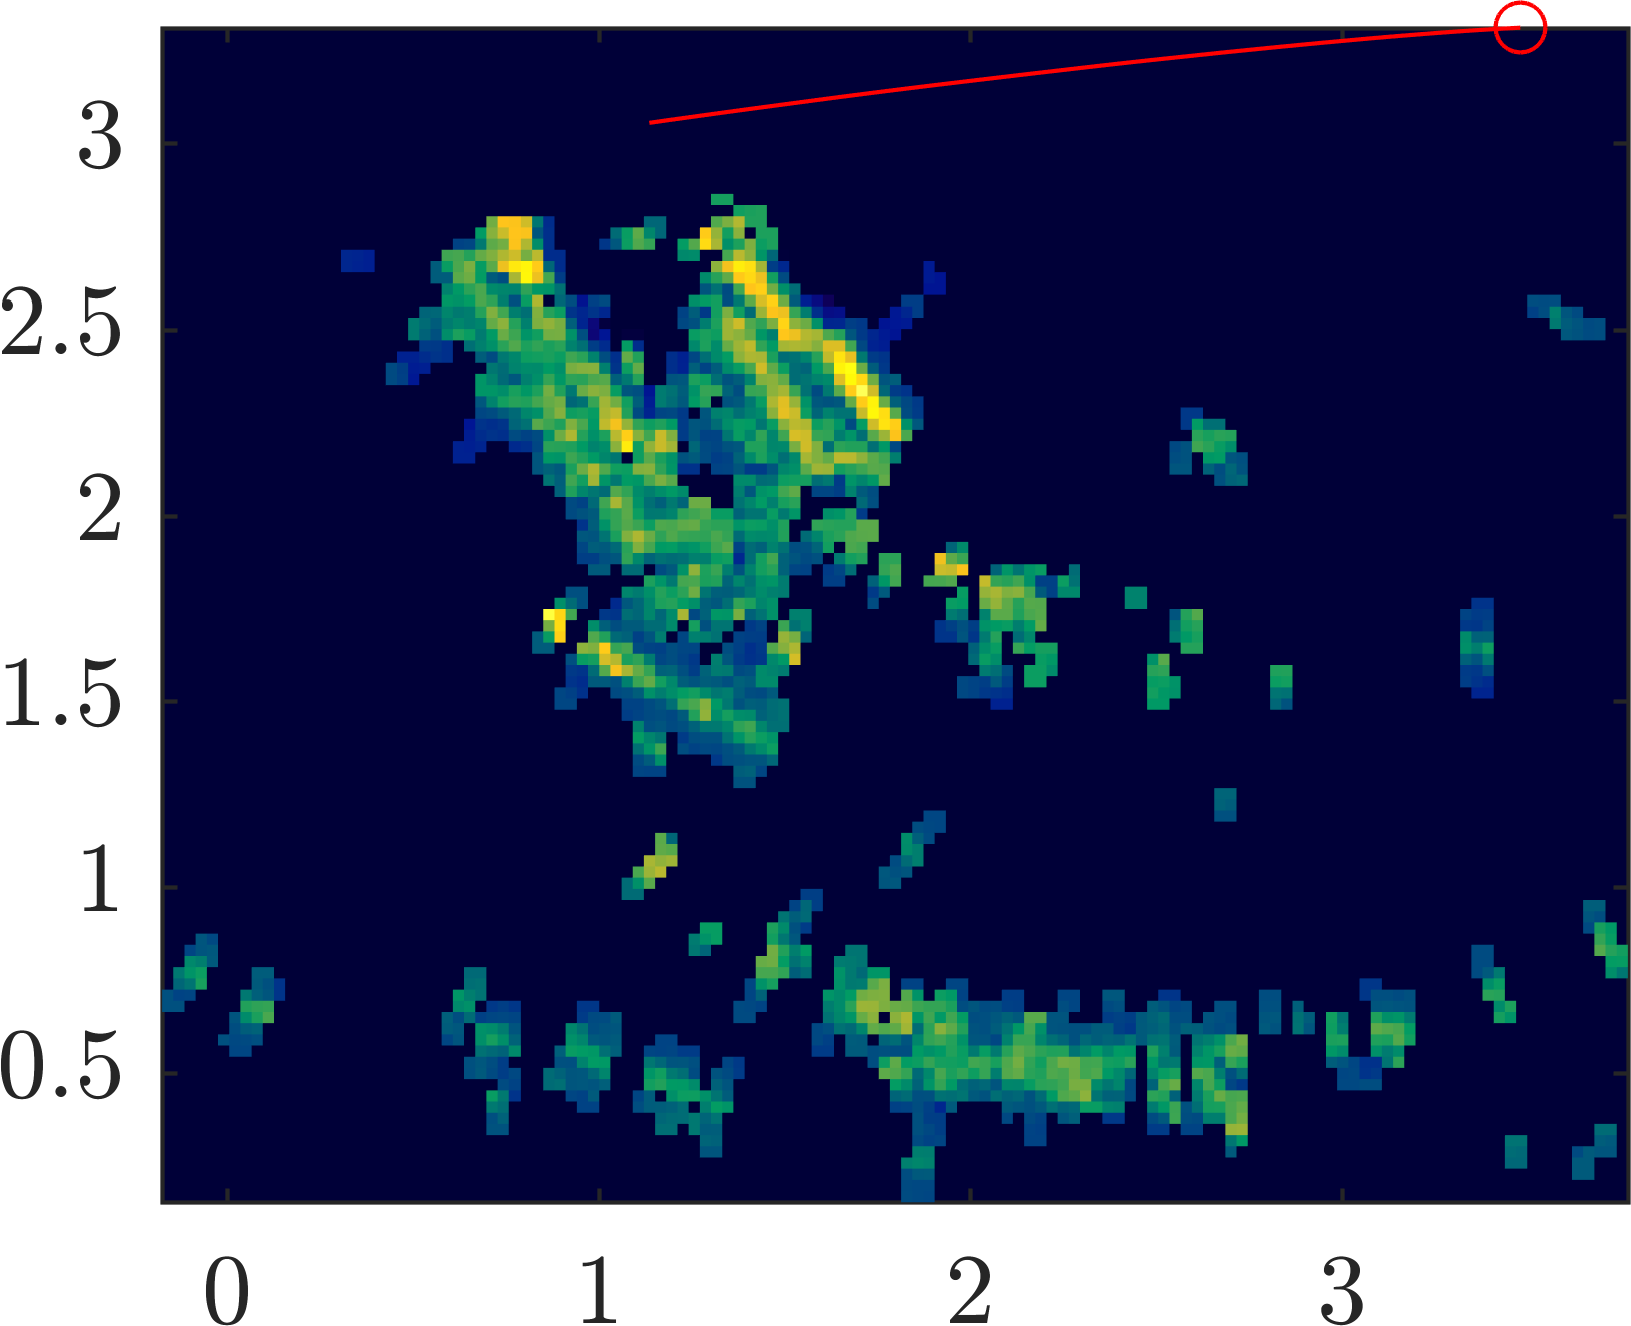
\includegraphics[width=\linewidth,max height=.475\textheight]{gfx/results/garden_reprojection.png}
    \end{subfigure}%
    \caption{Garden scan}
\end{figure}

\begin{figure}[htbp]
    \centering
    \begin{subfigure}[t]{0.475\linewidth}
        \centering
        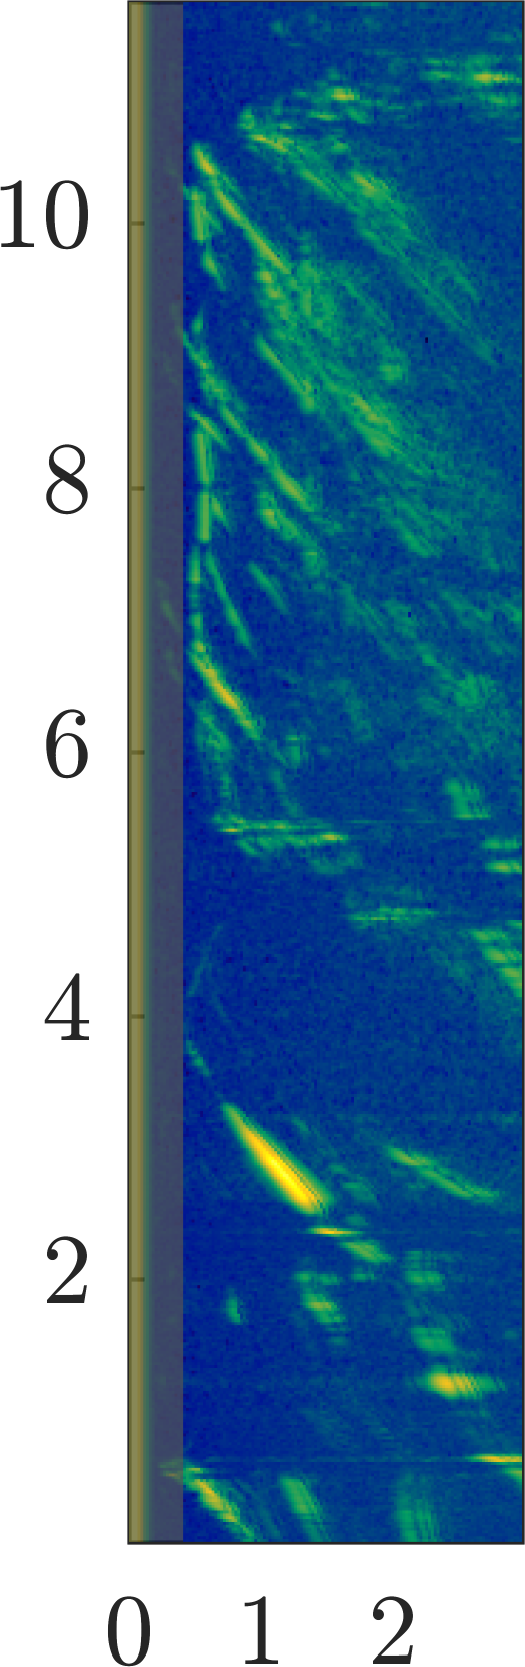
\includegraphics[width=\linewidth,max height=.475\textheight]{gfx/results/homecinema_input.png}
    \end{subfigure}%
    \hfill%
    \begin{subfigure}[t]{0.475\linewidth}  
        \centering 
        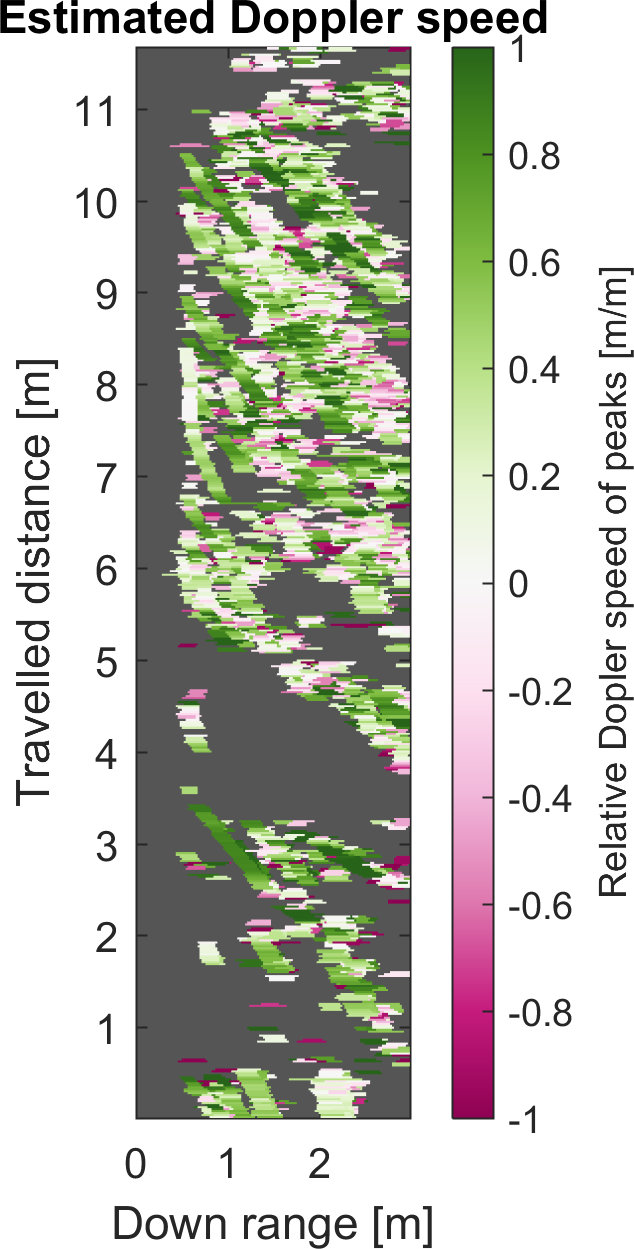
\includegraphics[width=\linewidth,max height=.475\textheight]{gfx/results/homecinema_doppler.png}
    \end{subfigure}\bigskip\\
    \begin{subfigure}[t]{0.5\linewidth}   
        \centering 
        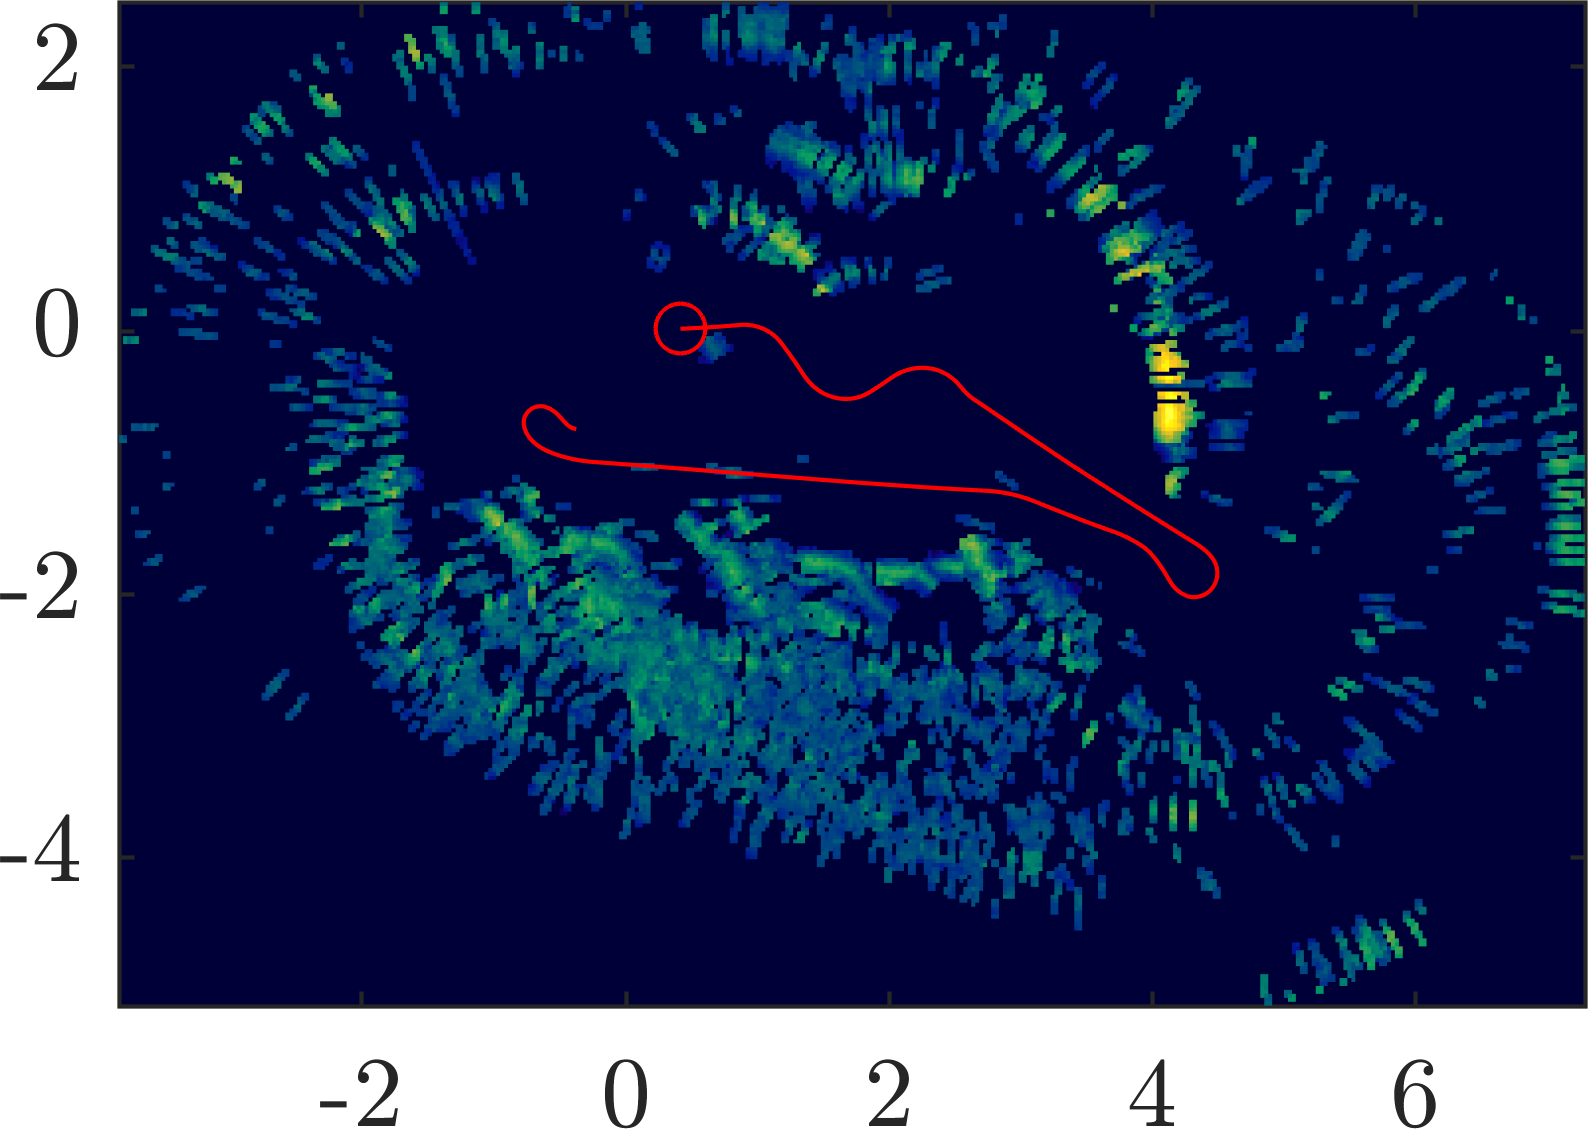
\includegraphics[width=\linewidth,max height=.475\textheight]{gfx/results/homecinema_reprojection.png}
    \end{subfigure}%
    \caption{Home Cinema scan}
\end{figure}

\begin{figure}[htbp]
    \centering
    \begin{subfigure}[t]{0.475\linewidth}
        \centering
        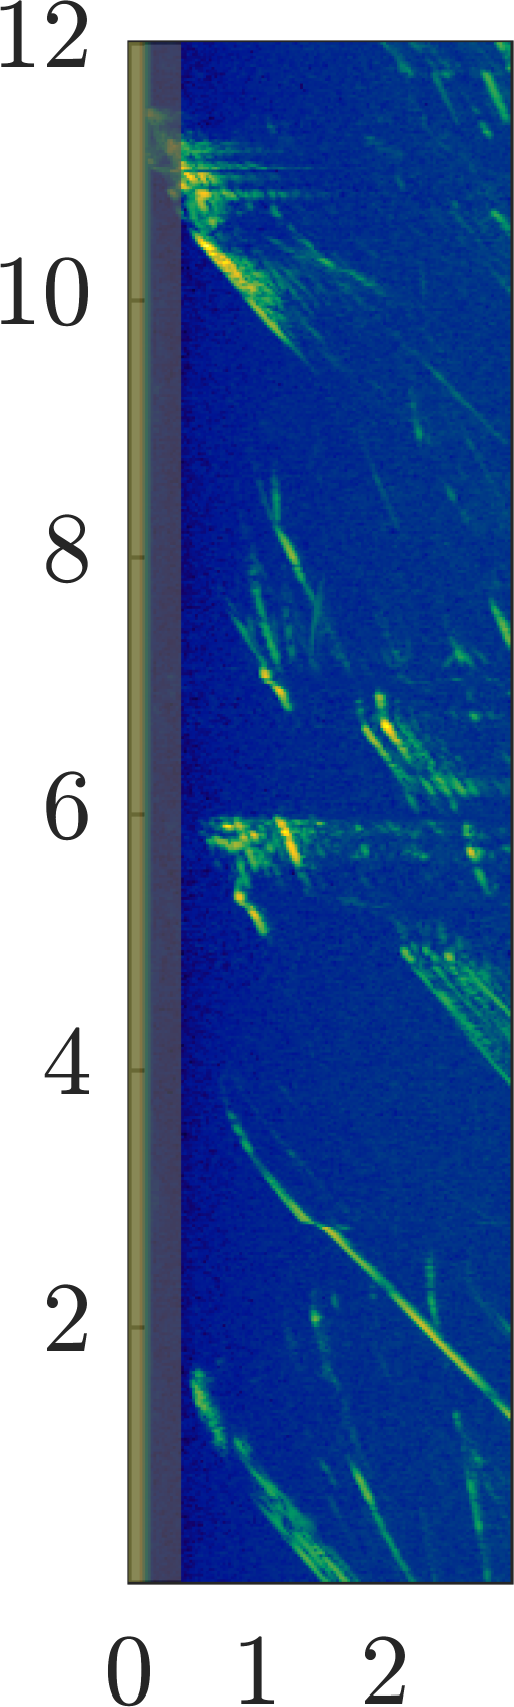
\includegraphics[width=\linewidth,max height=.475\textheight]{gfx/results/indoorswimmingpool_input.png}
    \end{subfigure}%
    \hfill%
    \begin{subfigure}[t]{0.475\linewidth}  
        \centering 
        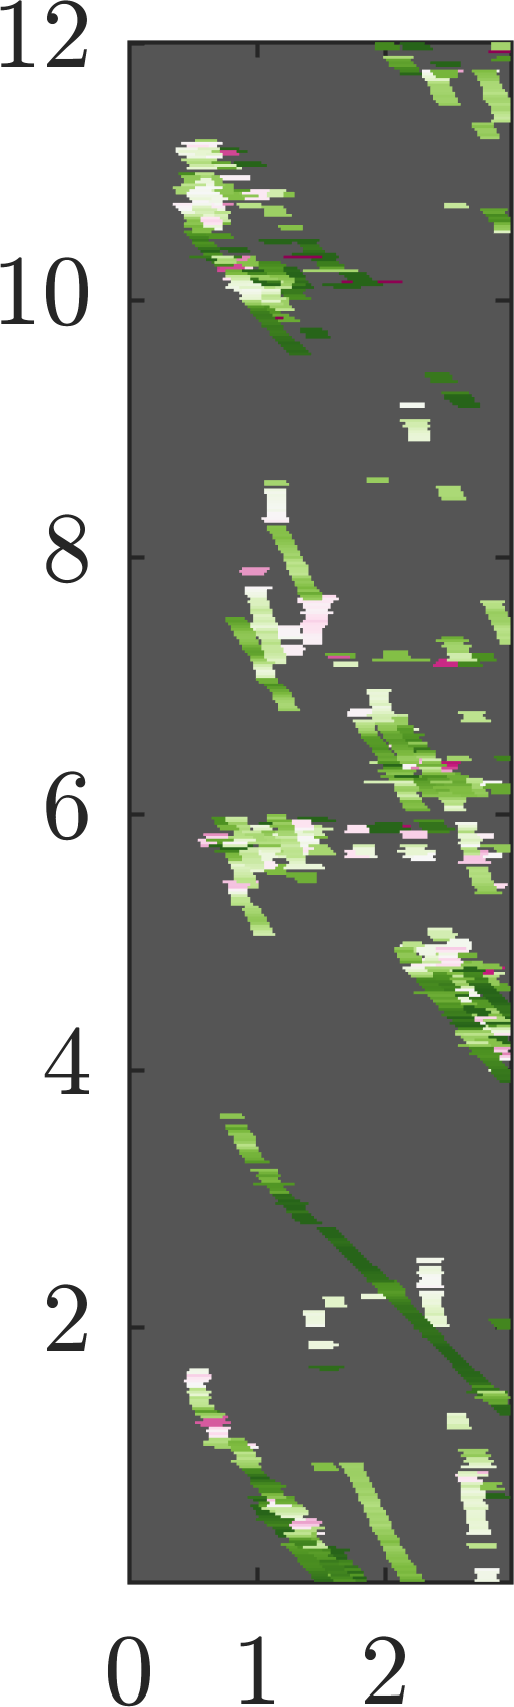
\includegraphics[width=\linewidth,max height=.475\textheight]{gfx/results/indoorswimmingpool_doppler.png}
    \end{subfigure}\bigskip\\
    \begin{subfigure}[t]{0.5\linewidth}   
        \centering 
        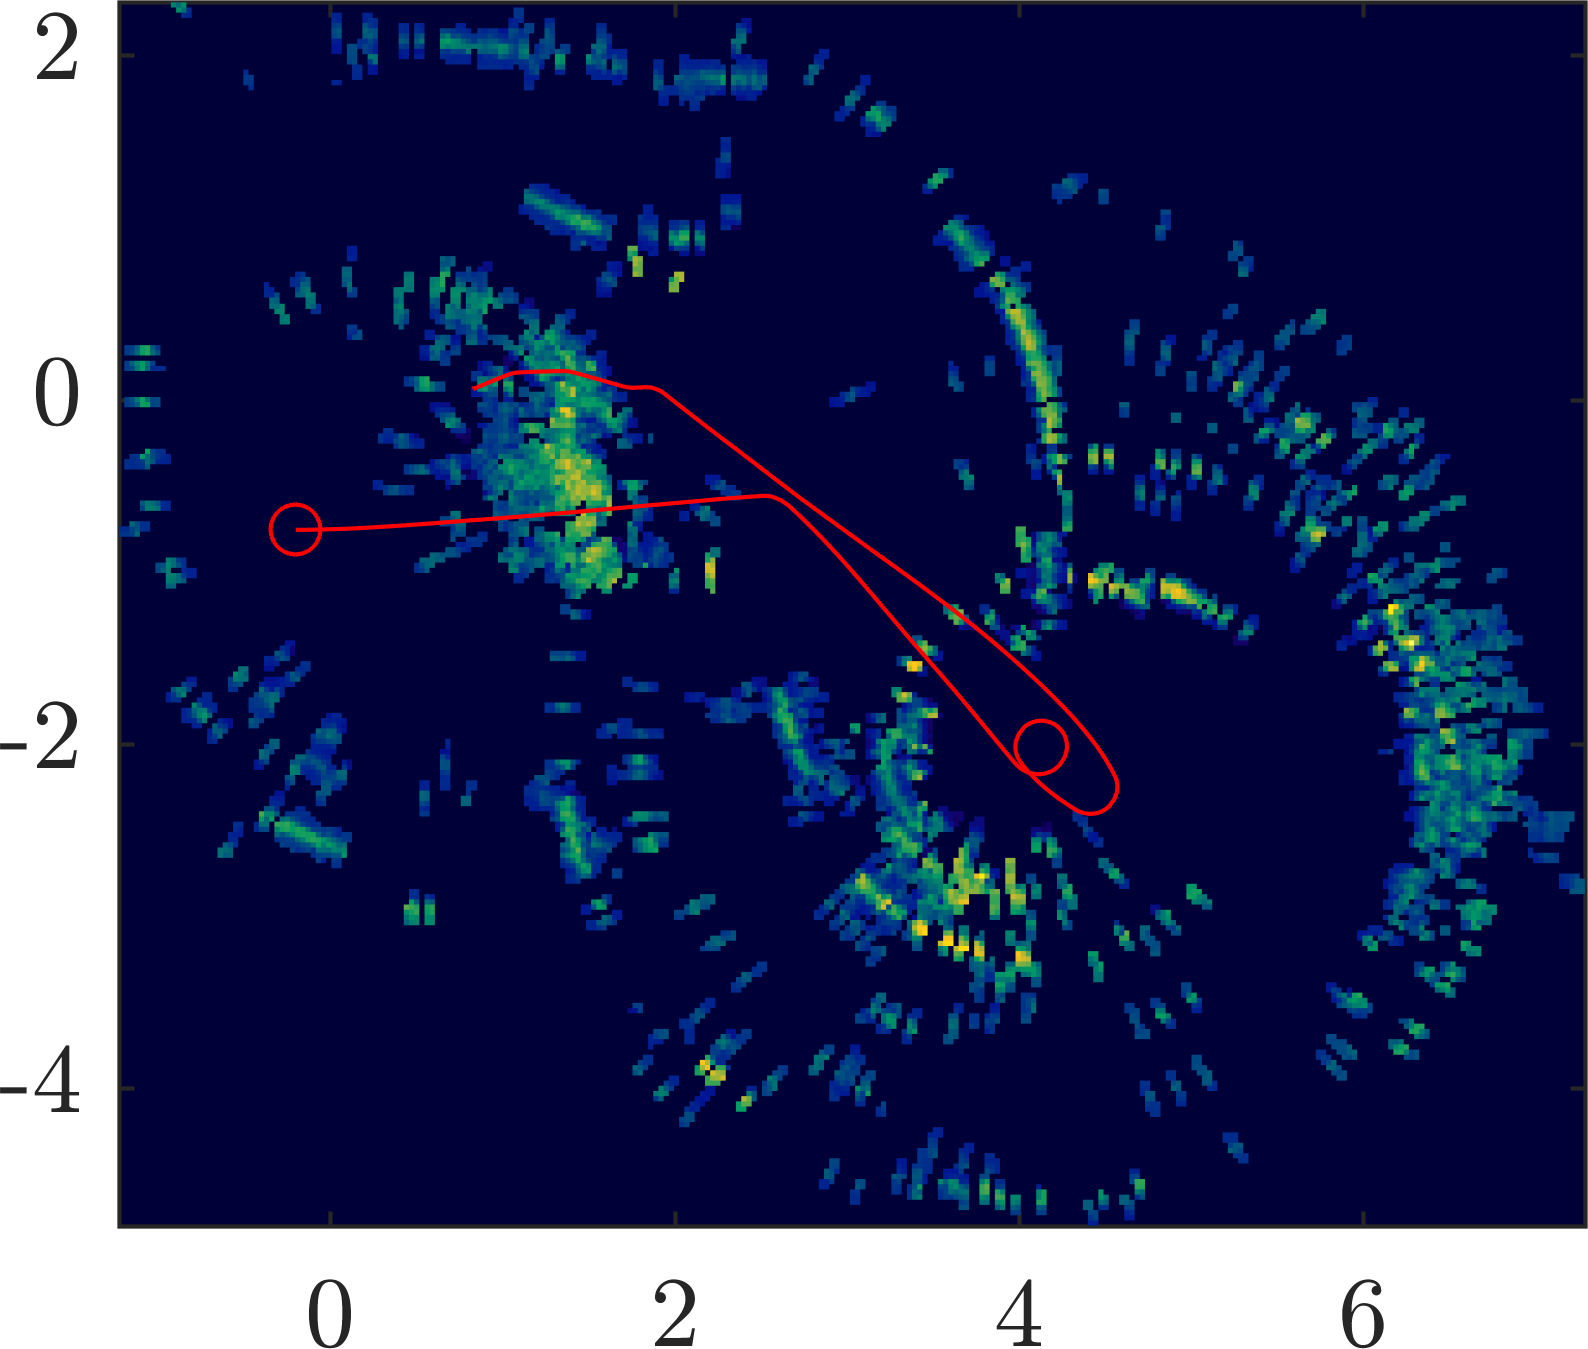
\includegraphics[width=\linewidth,max height=.475\textheight]{gfx/results/indoorswimmingpool_reprojection.png}
    \end{subfigure}%
    \caption{Inddor Swimming Pool scan}
\end{figure}

\begin{figure}[htbp]
    \centering
    \begin{subfigure}[t]{0.475\linewidth}
        \centering
        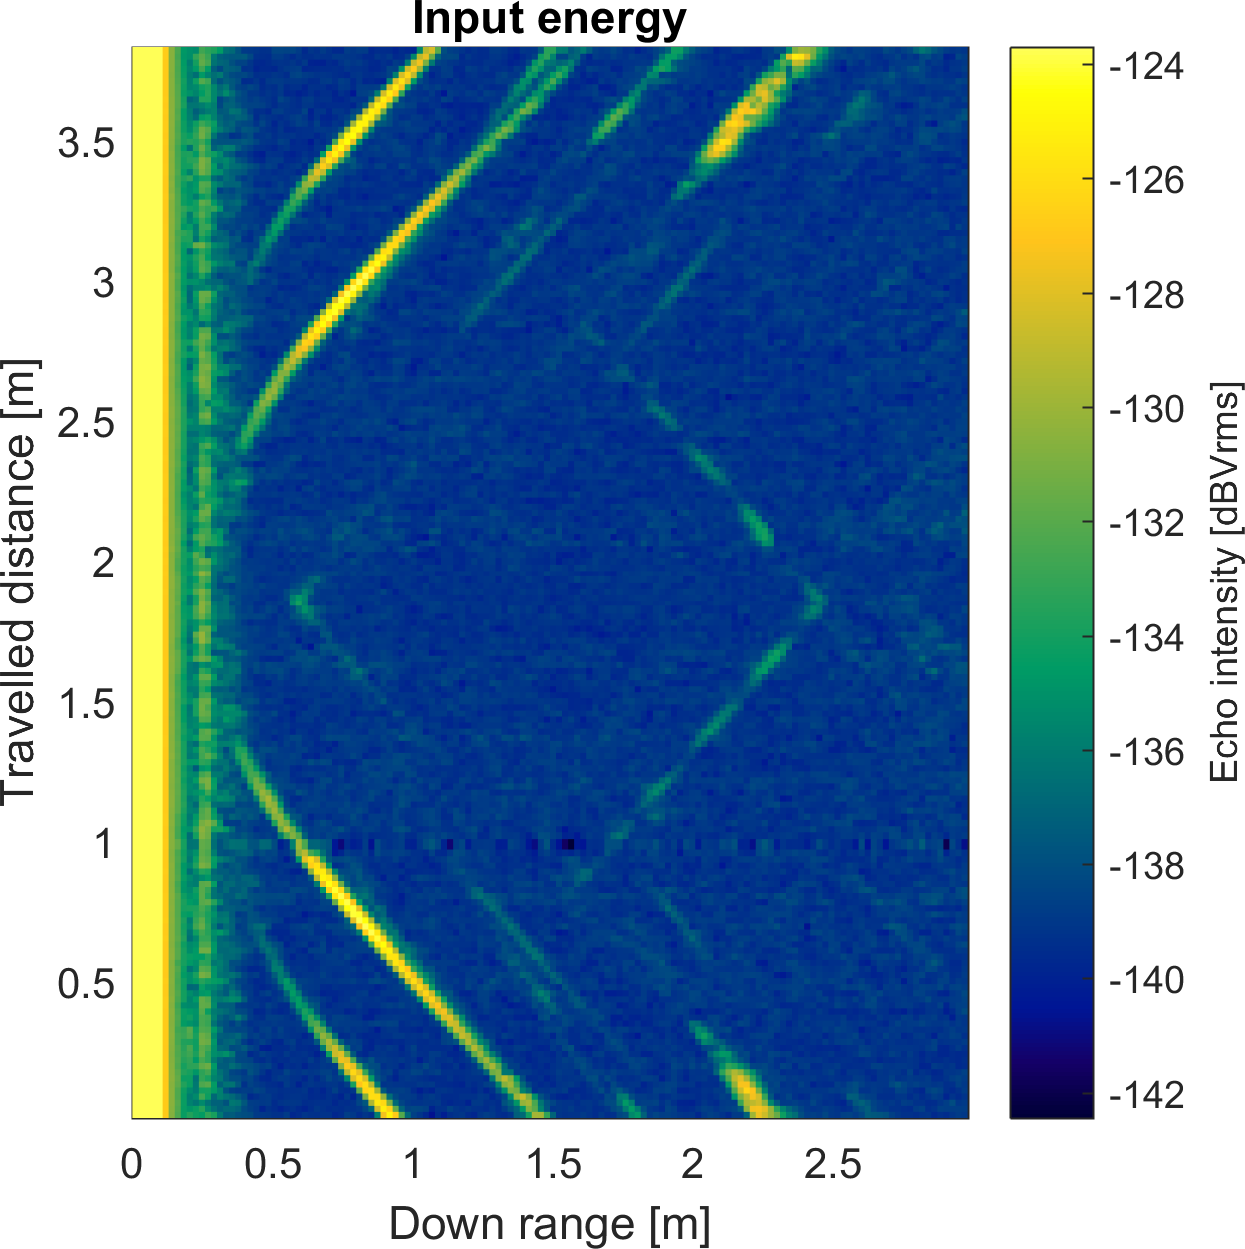
\includegraphics[width=\linewidth,max height=.475\textheight]{gfx/results/jailcell_input.png}
    \end{subfigure}%
    \hfill%
    \begin{subfigure}[t]{0.475\linewidth}  
        \centering 
        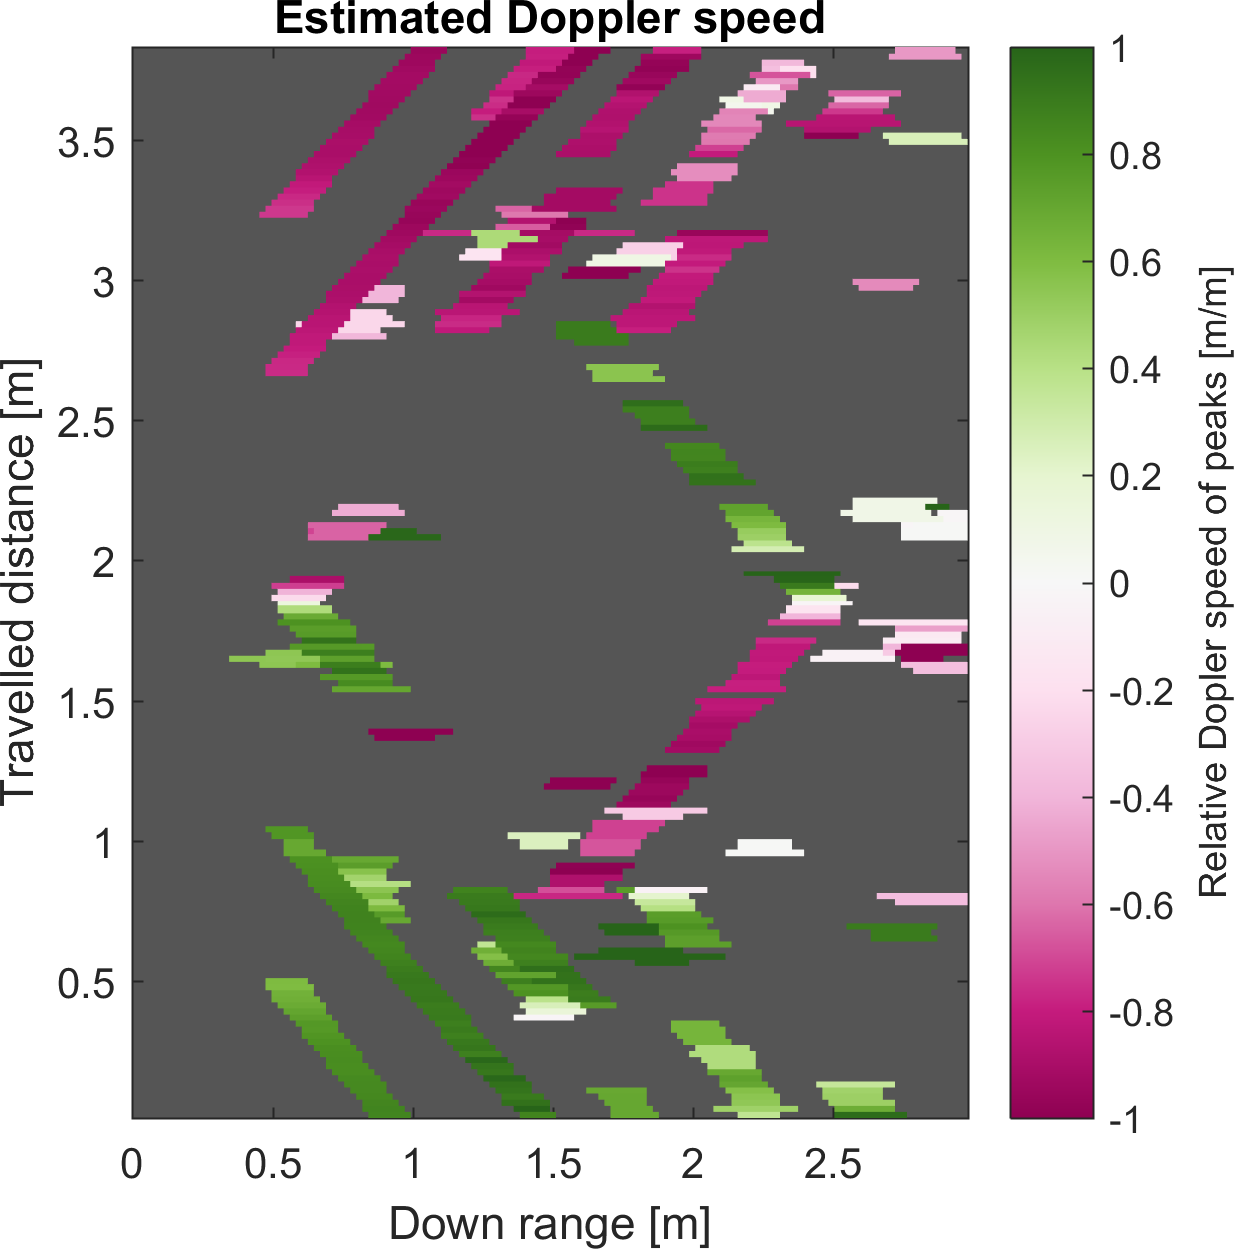
\includegraphics[width=\linewidth,max height=.475\textheight]{gfx/results/jailcell_doppler.png}
    \end{subfigure}\bigskip\\
    \begin{subfigure}[t]{0.5\linewidth}   
        \centering 
        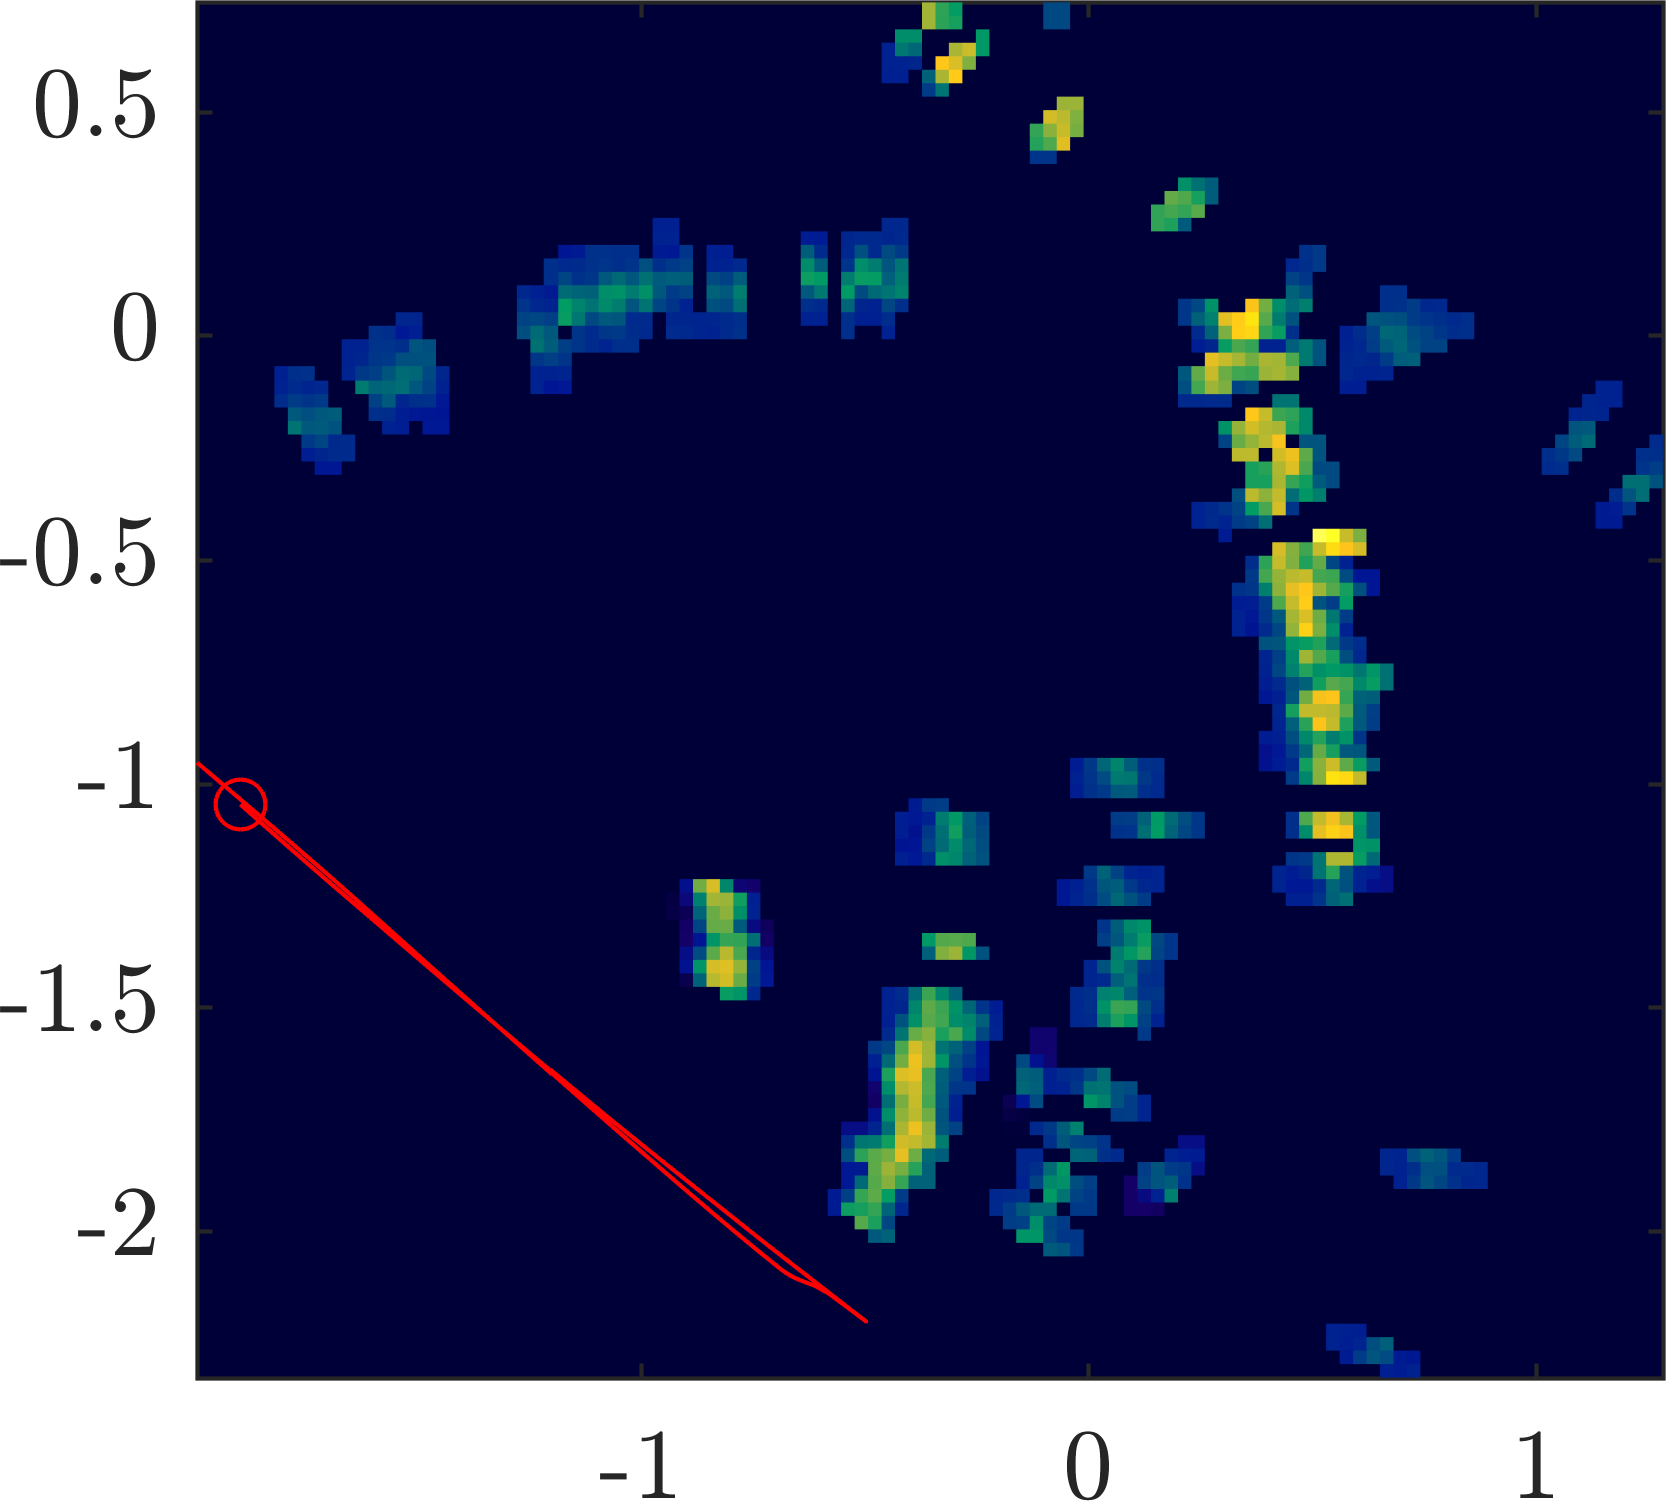
\includegraphics[width=\linewidth,max height=.475\textheight]{gfx/results/jailcell_reprojection.png}
    \end{subfigure}%
    \caption{Jail Cell scan}
    \label{fig:res_j}
\end{figure}

\begin{figure}[htbp]
    \centering
    \begin{subfigure}[t]{0.475\linewidth}
        \centering
        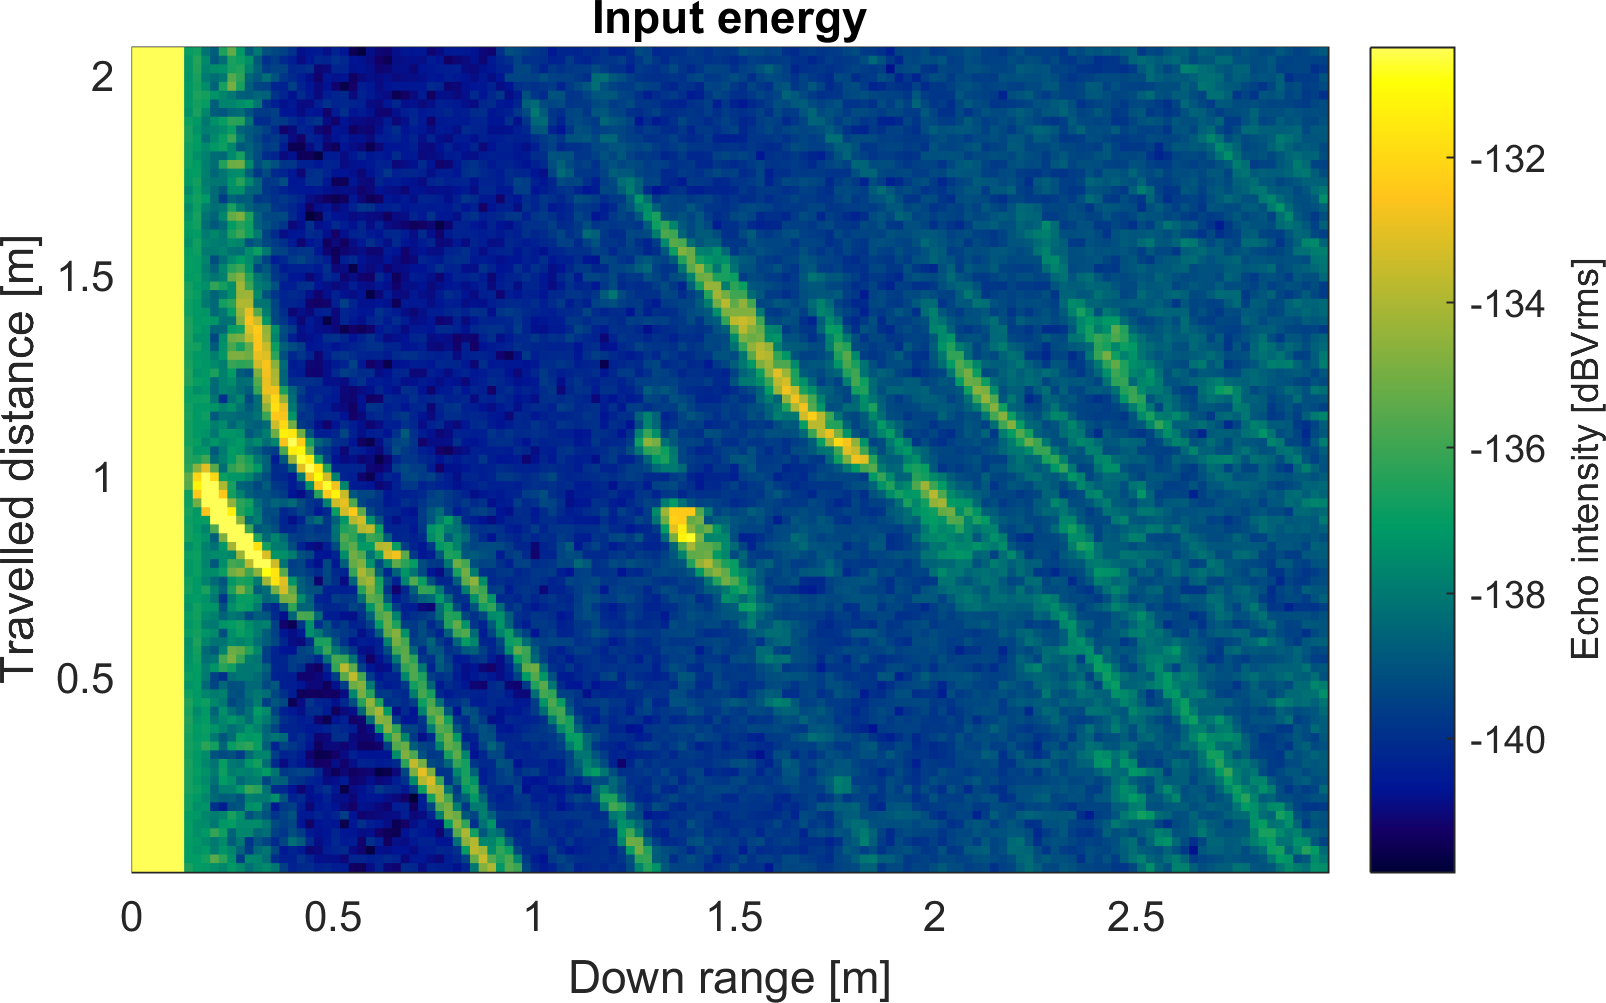
\includegraphics[width=\linewidth,max height=.475\textheight]{gfx/results/kitchen_input.png}
    \end{subfigure}%
    \hfill%
    \begin{subfigure}[t]{0.475\linewidth}  
        \centering 
        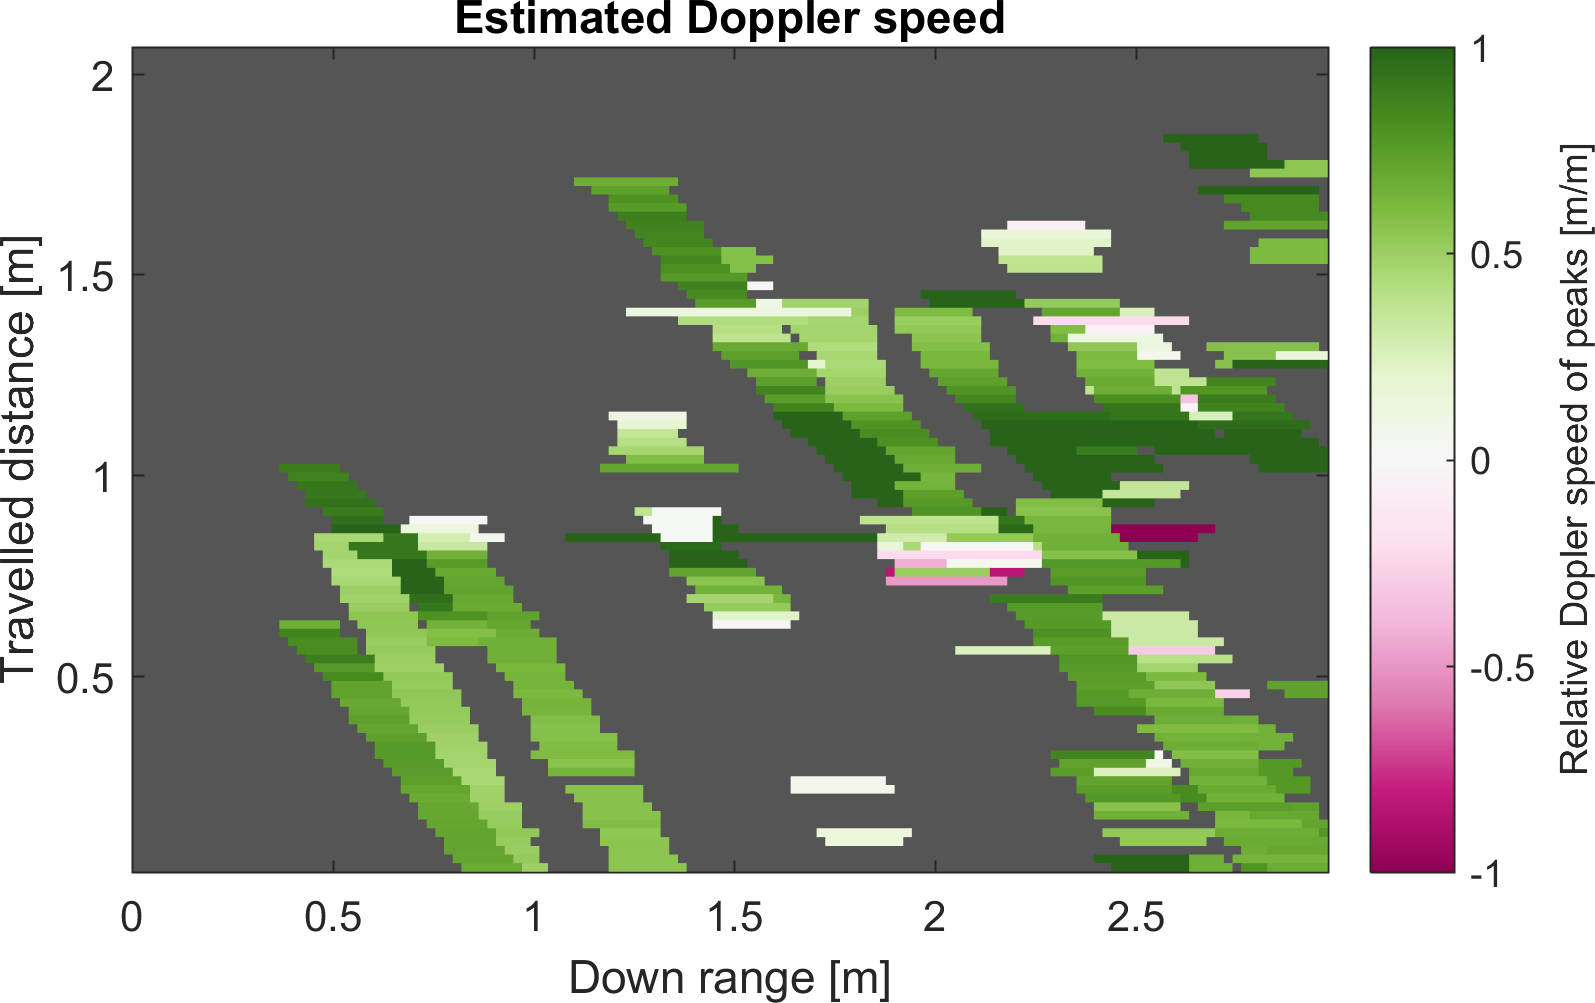
\includegraphics[width=\linewidth,max height=.475\textheight]{gfx/results/kitchen_doppler.png}
    \end{subfigure}\bigskip\\
    \begin{subfigure}[t]{0.5\linewidth}   
        \centering 
        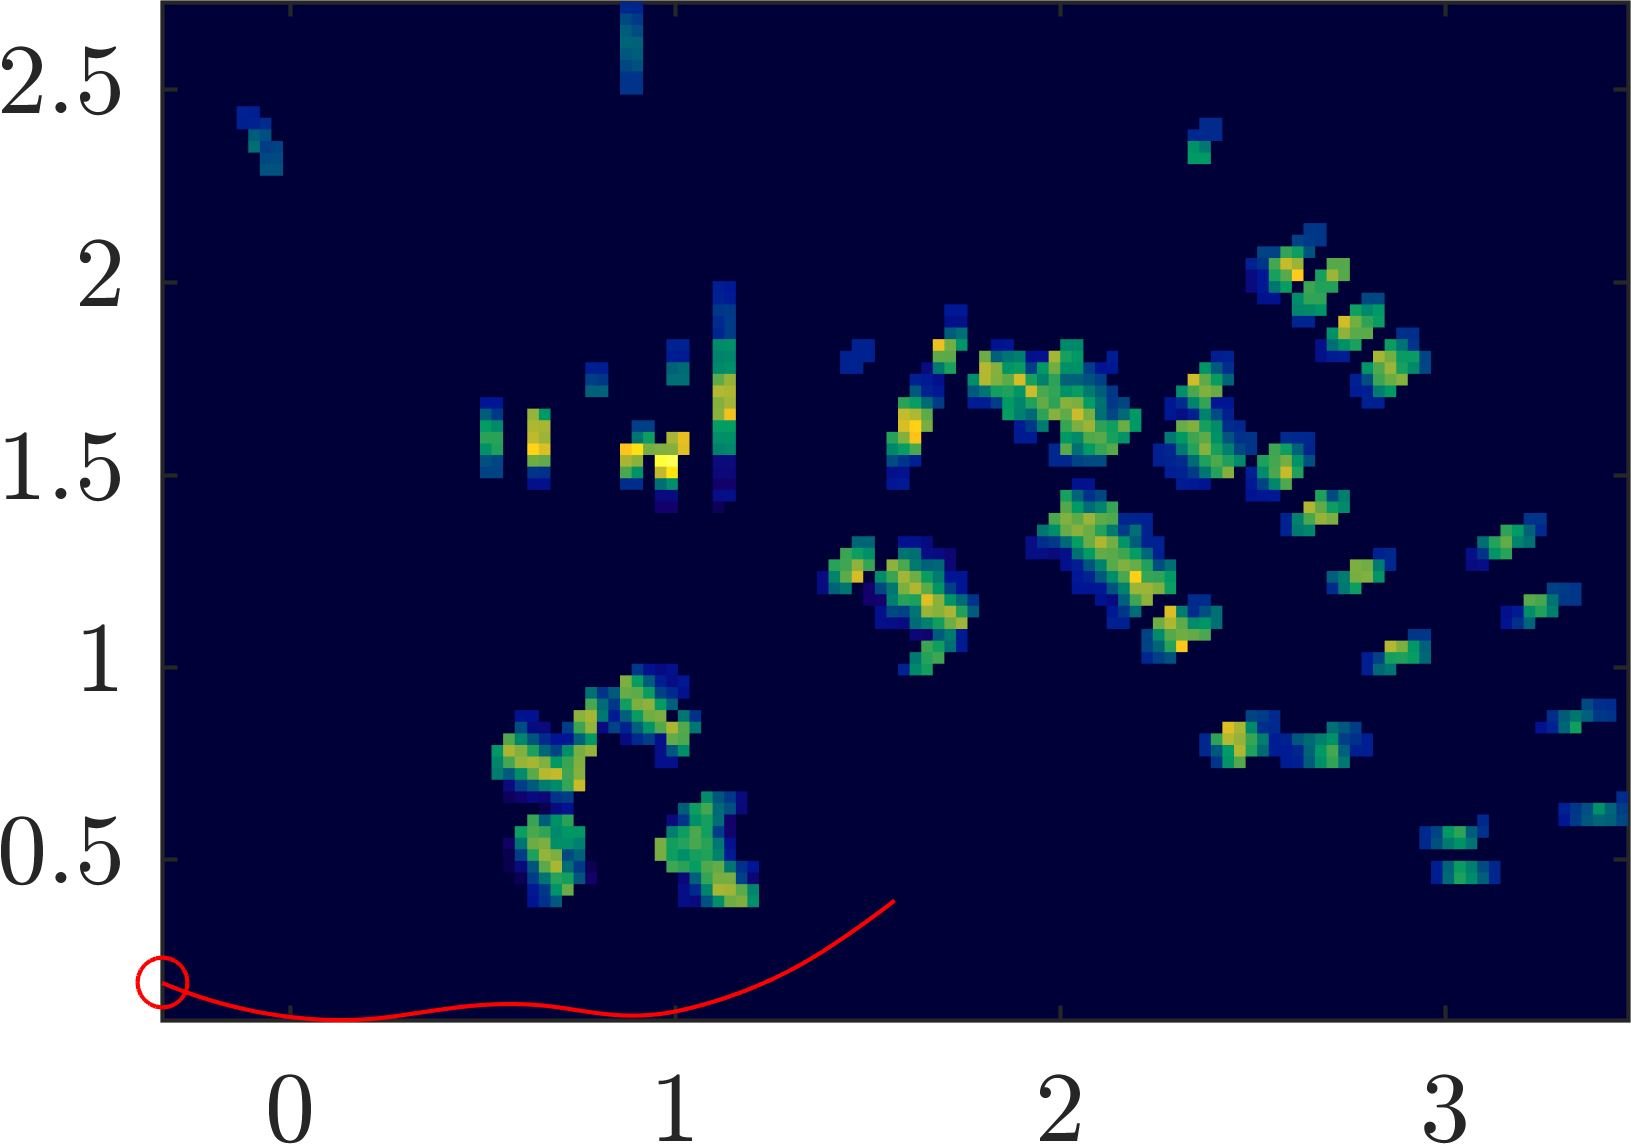
\includegraphics[width=\linewidth,max height=.475\textheight]{gfx/results/kitchen_reprojection.png}
    \end{subfigure}%
    \caption{Kitchen scan}
\end{figure}

\begin{figure}[htbp]
    \centering
    \begin{subfigure}[t]{0.475\linewidth}
        \centering
        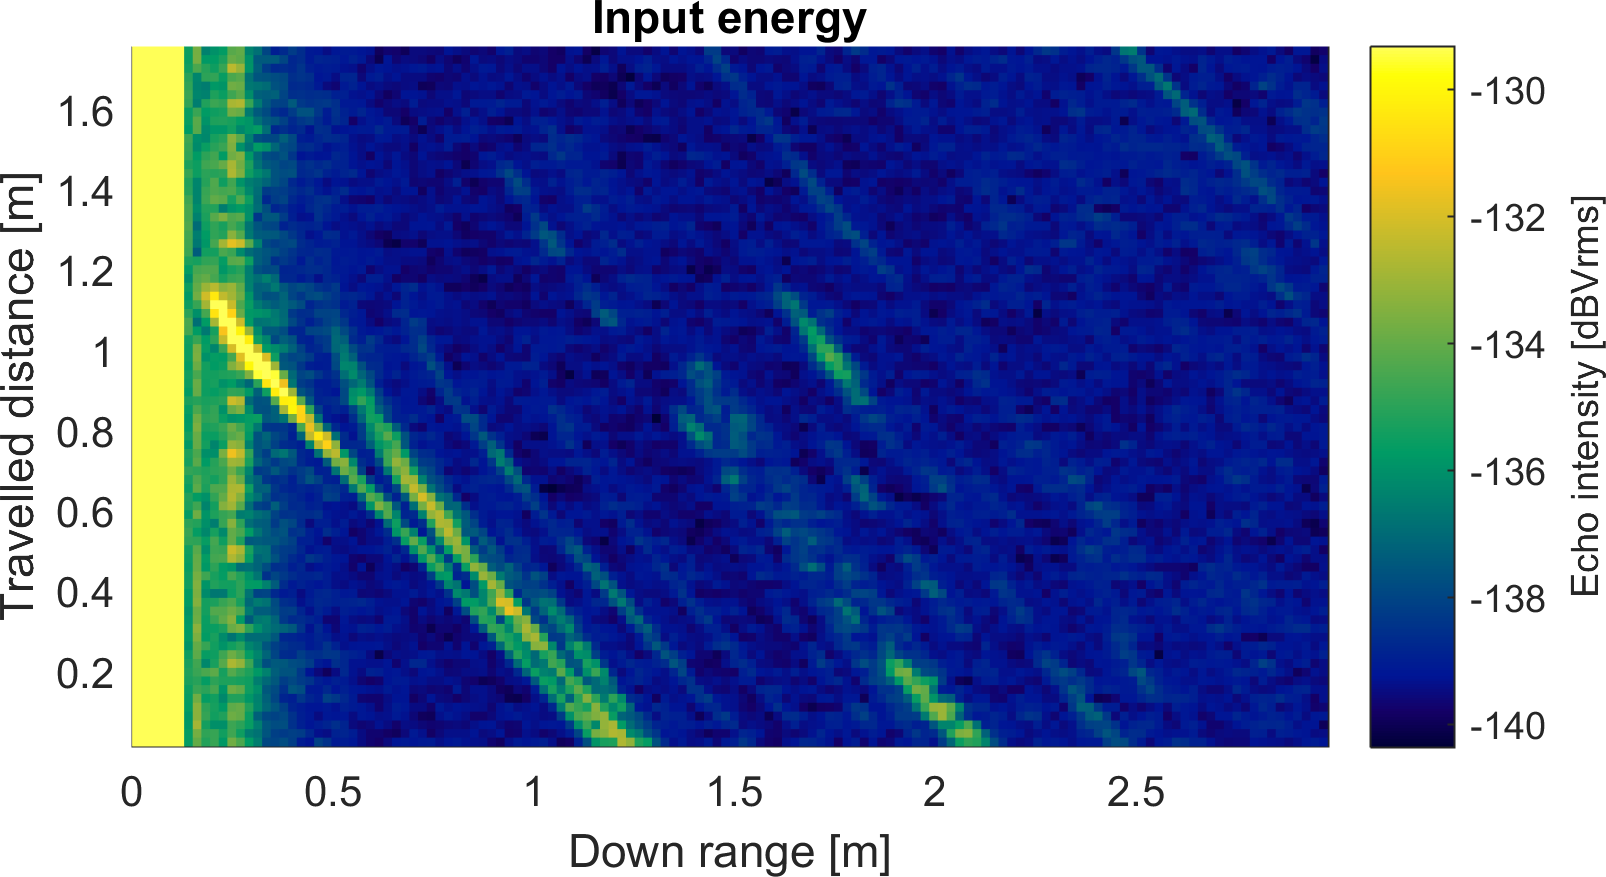
\includegraphics[width=\linewidth,max height=.475\textheight]{gfx/results/lobby_input.png}
    \end{subfigure}%
    \hfill%
    \begin{subfigure}[t]{0.475\linewidth}
        \centering
        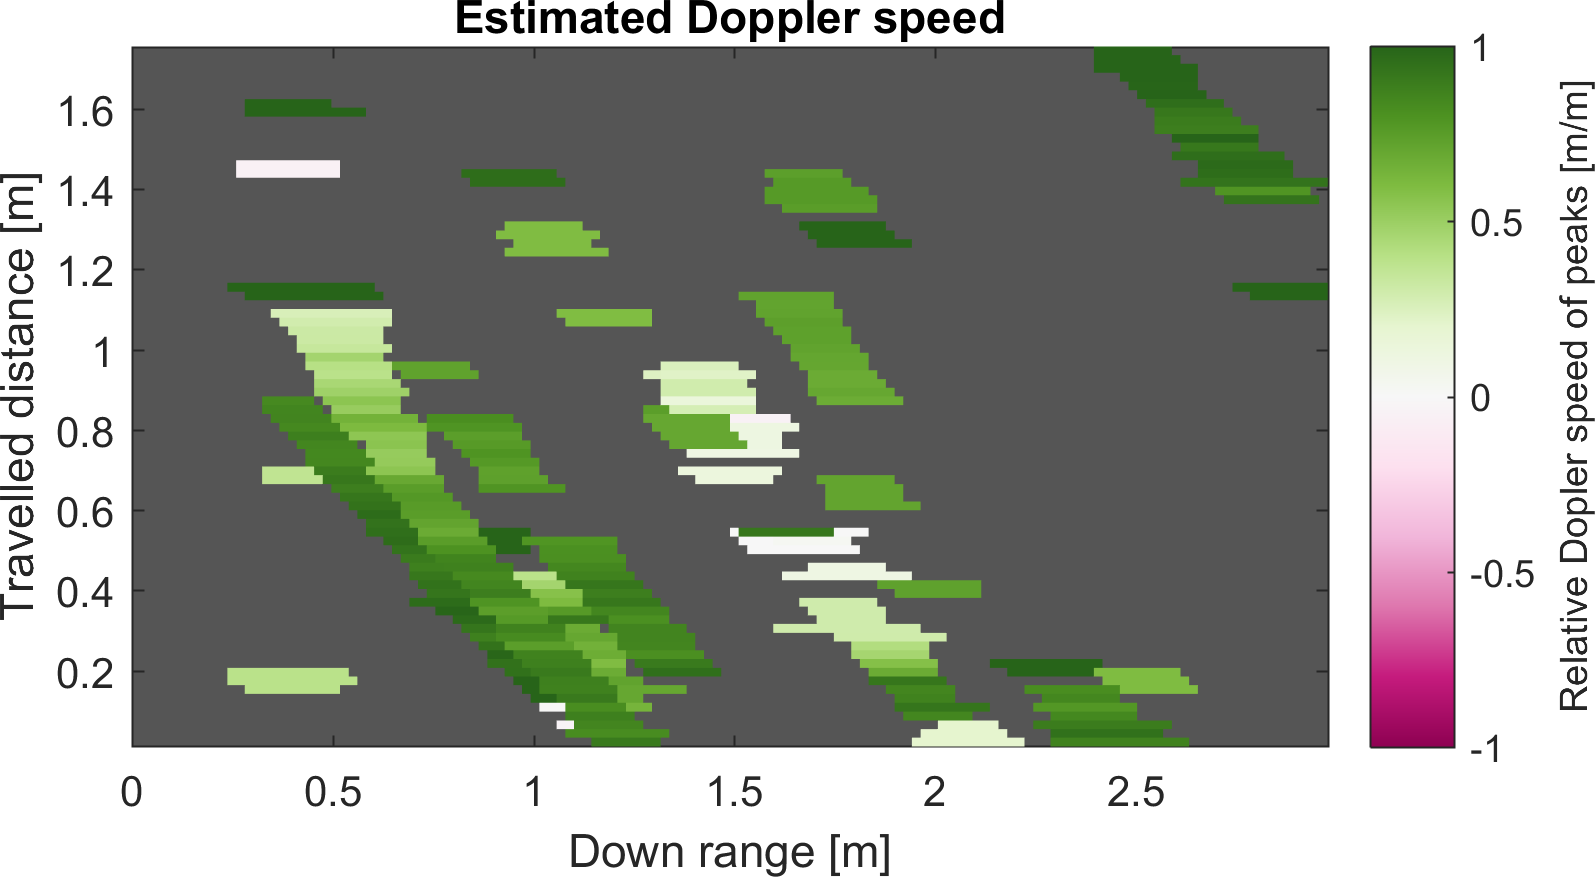
\includegraphics[width=\linewidth,max height=.475\textheight]{gfx/results/lobby_doppler.png}
    \end{subfigure}\bigskip\\
    \begin{subfigure}[t]{0.475\linewidth}  
        \centering 
        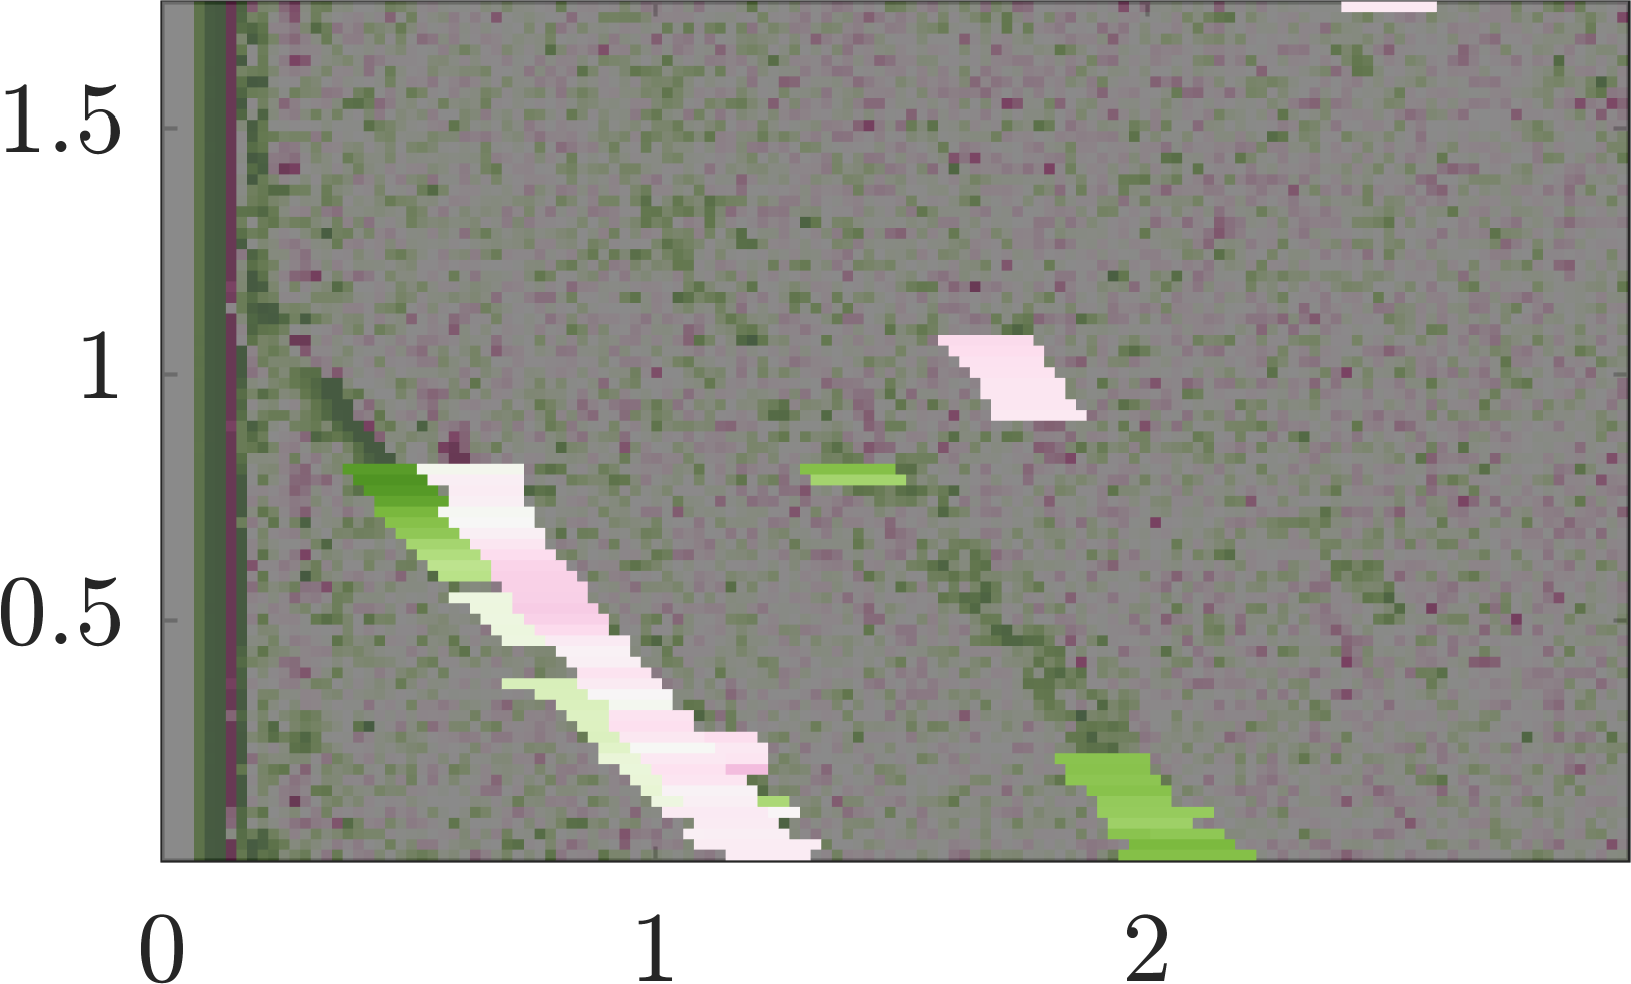
\includegraphics[width=\linewidth,max height=.475\textheight]{gfx/results/lobby_doa.png}
    \end{subfigure}%
    \hfill%
    \begin{subfigure}[t]{0.475\linewidth}   
        \centering 
        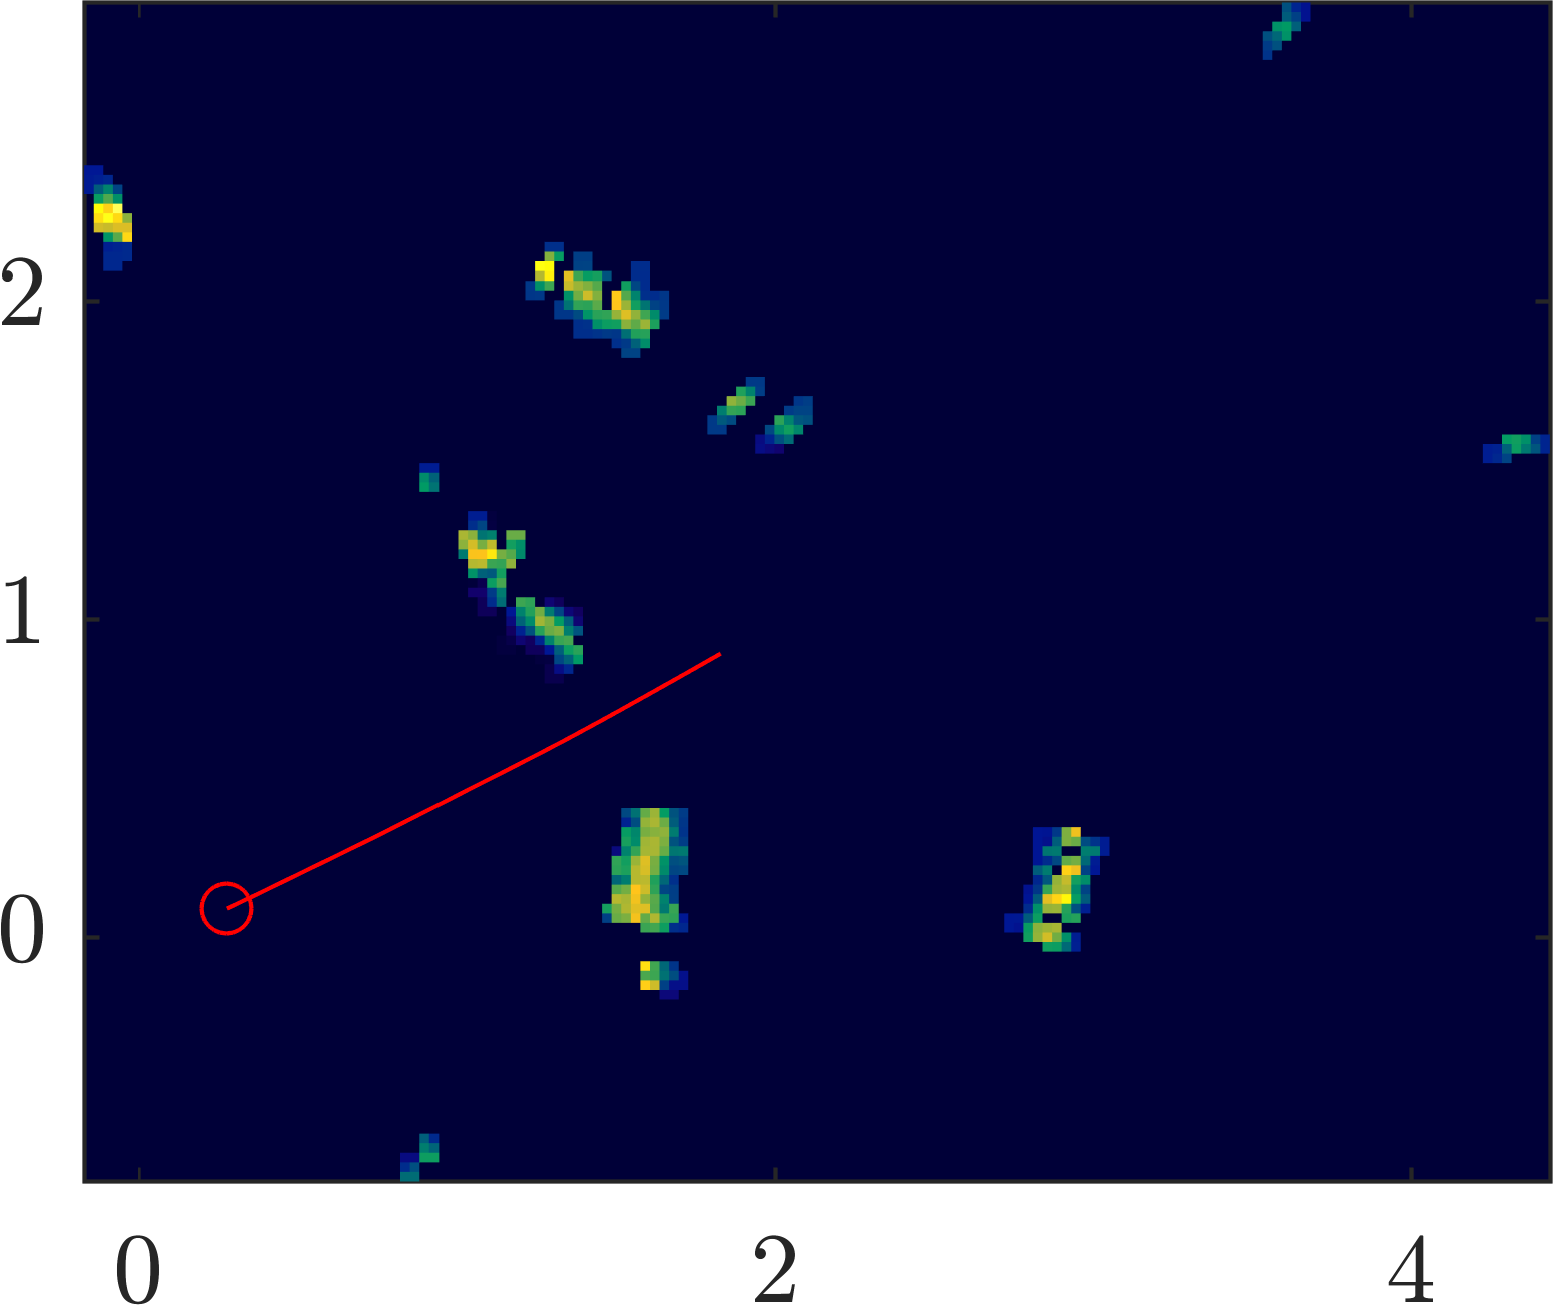
\includegraphics[width=\linewidth,max height=.475\textheight]{gfx/results/lobby_reprojection.png}
    \end{subfigure}%
    \caption{Lobby scan}
\end{figure}

\begin{figure}[htbp]
    \centering
    \begin{subfigure}[t]{0.475\linewidth}
        \centering
        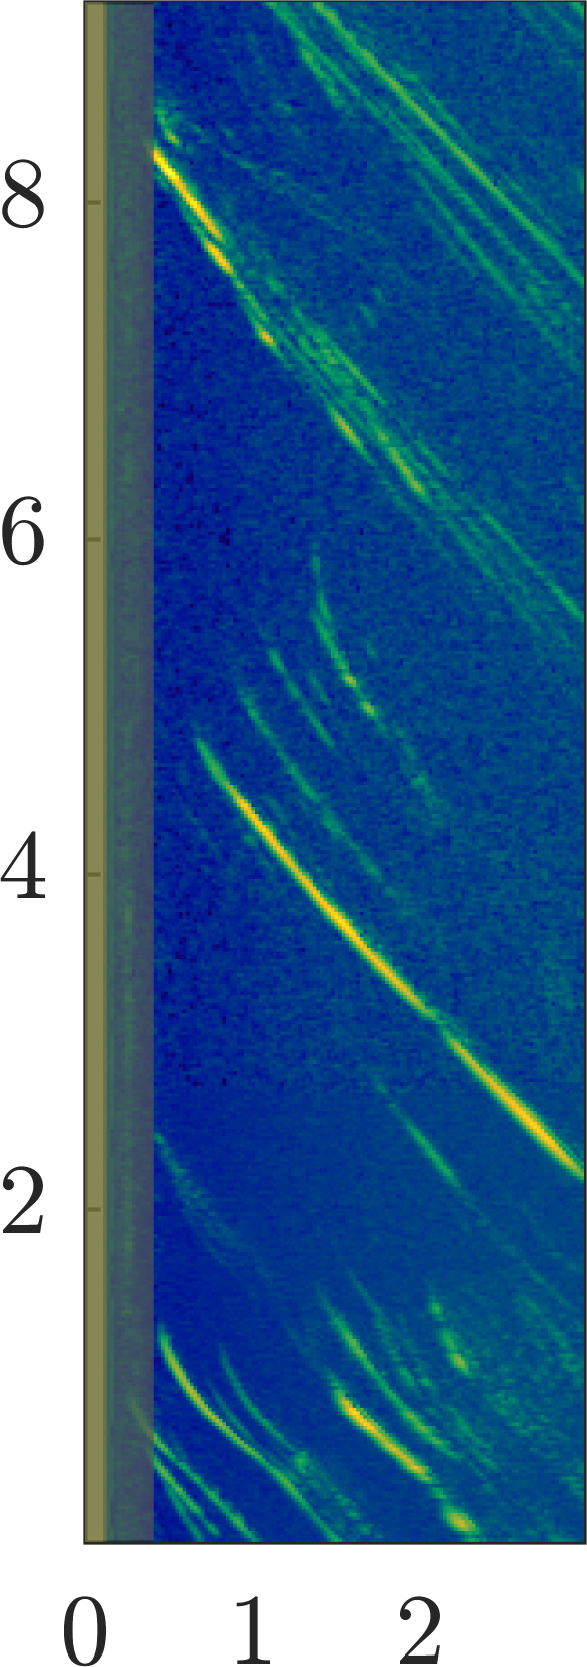
\includegraphics[width=\linewidth,max height=.475\textheight]{gfx/results/mancave_input.png}
    \end{subfigure}%
    \hfill%
    \begin{subfigure}[t]{0.475\linewidth}
        \centering
        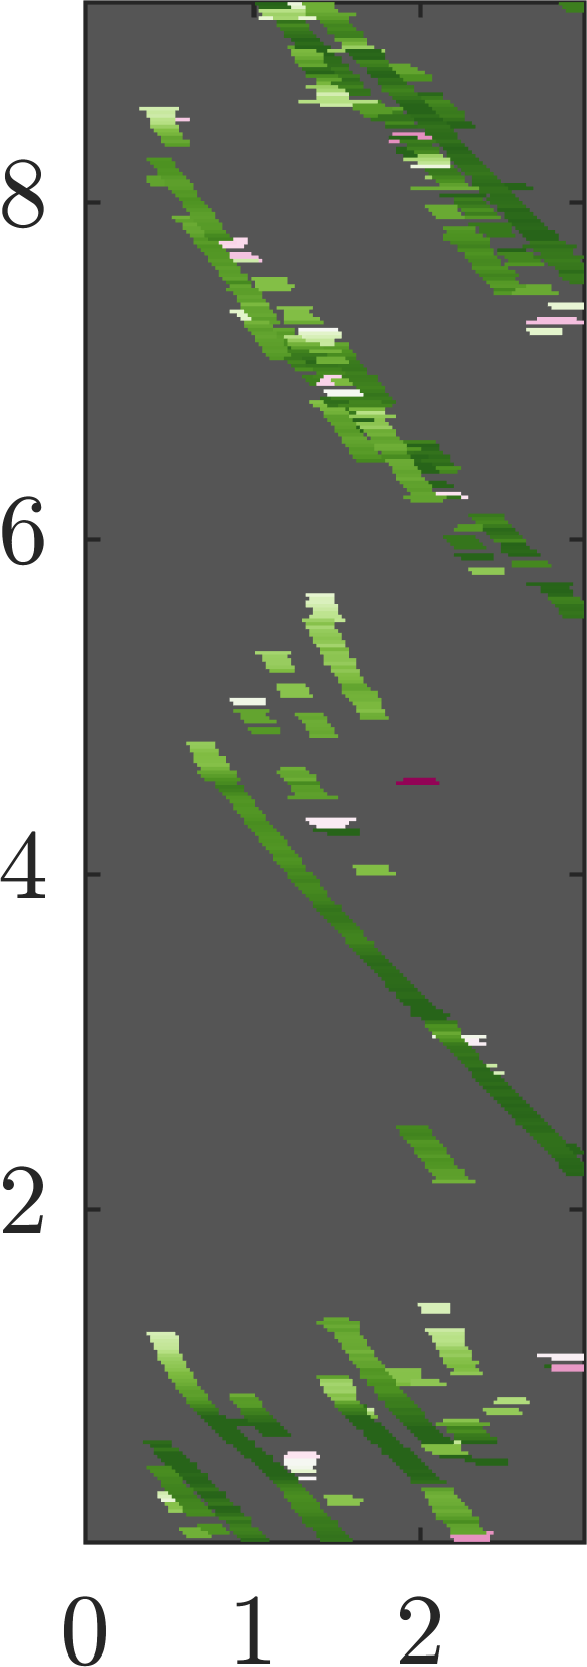
\includegraphics[width=\linewidth,max height=.475\textheight]{gfx/results/mancave_doppler.png}
    \end{subfigure}\bigskip\\
    \begin{subfigure}[t]{0.475\linewidth}  
        \centering 
        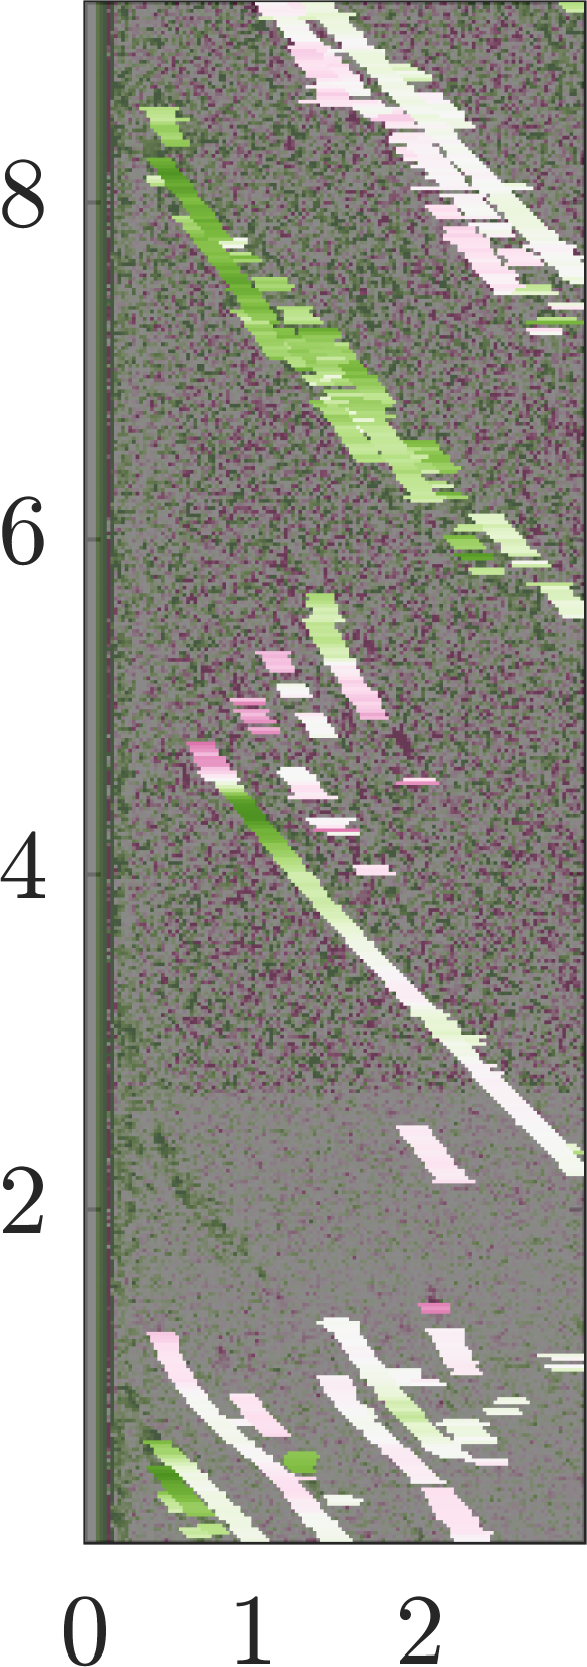
\includegraphics[width=\linewidth,max height=.475\textheight]{gfx/results/mancave_doa.png}
    \end{subfigure}%
    \hfill%
    \begin{subfigure}[t]{0.475\linewidth}   
        \centering 
        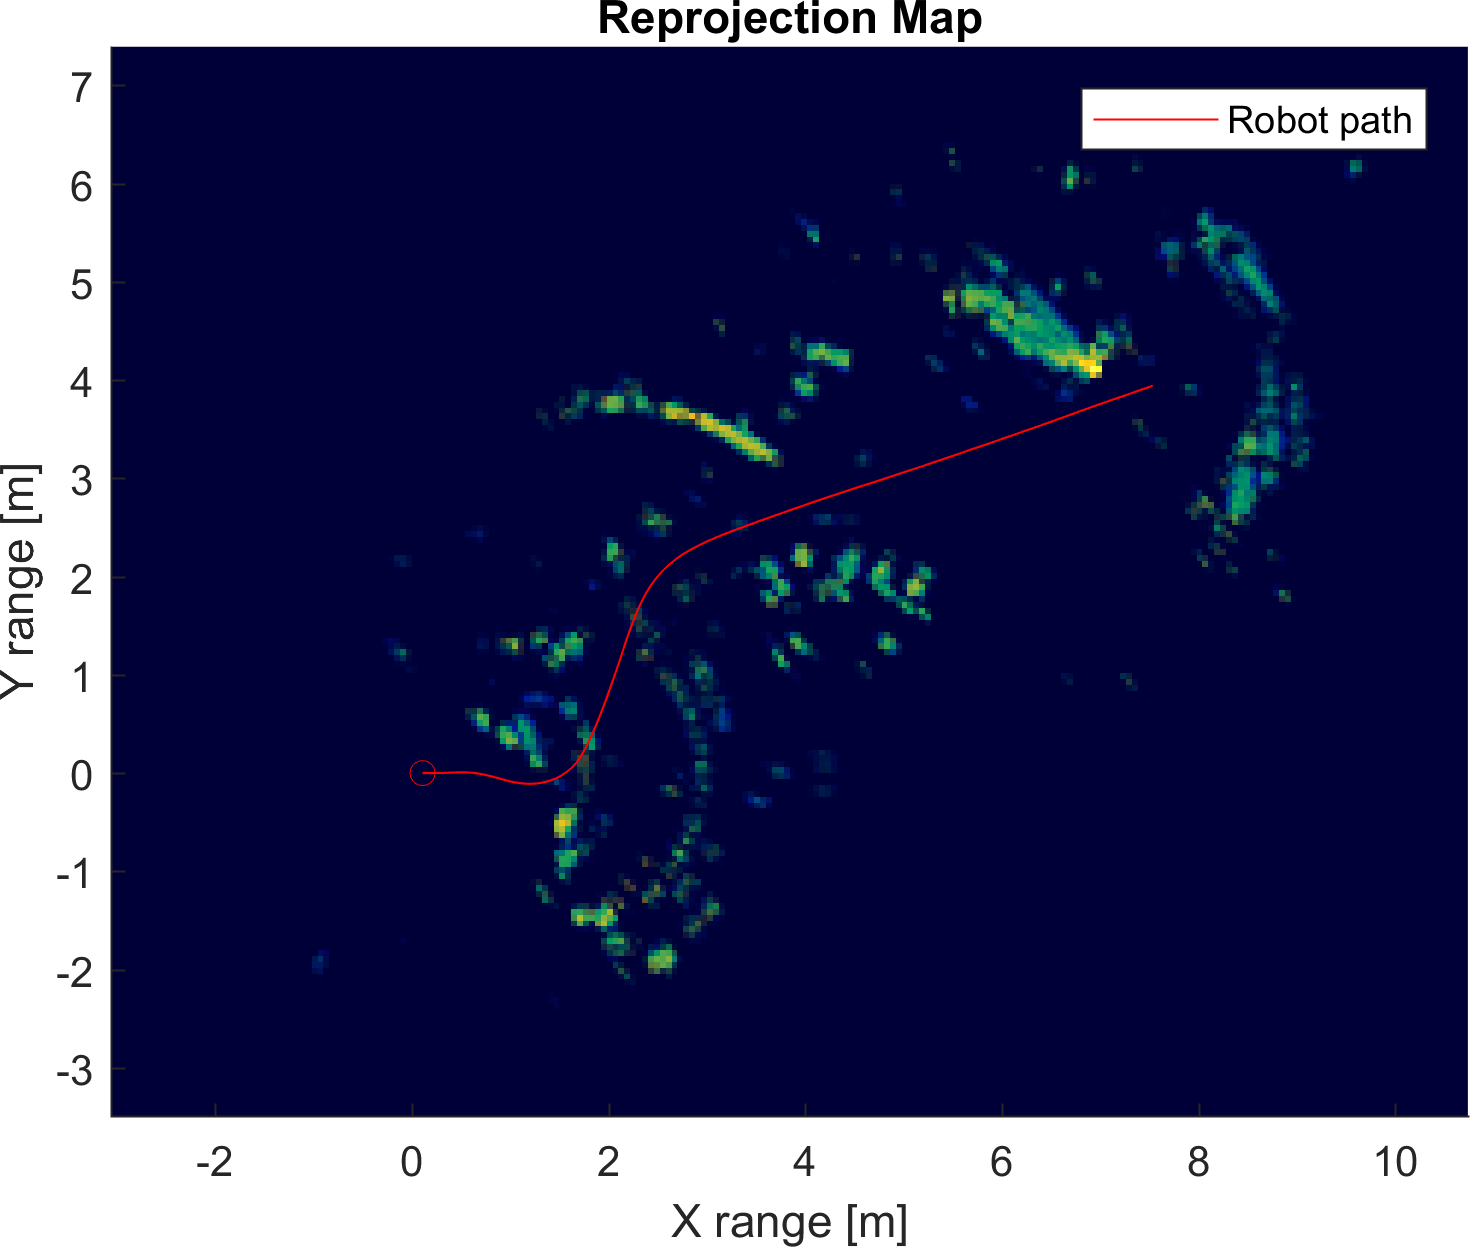
\includegraphics[width=\linewidth,max height=.475\textheight]{gfx/results/mancave_reprojection.png}
    \end{subfigure}%
    \caption{Mancave scan}
\end{figure}

\begin{figure}[htbp]
    \centering
    \begin{subfigure}[t]{0.475\linewidth}
        \centering
        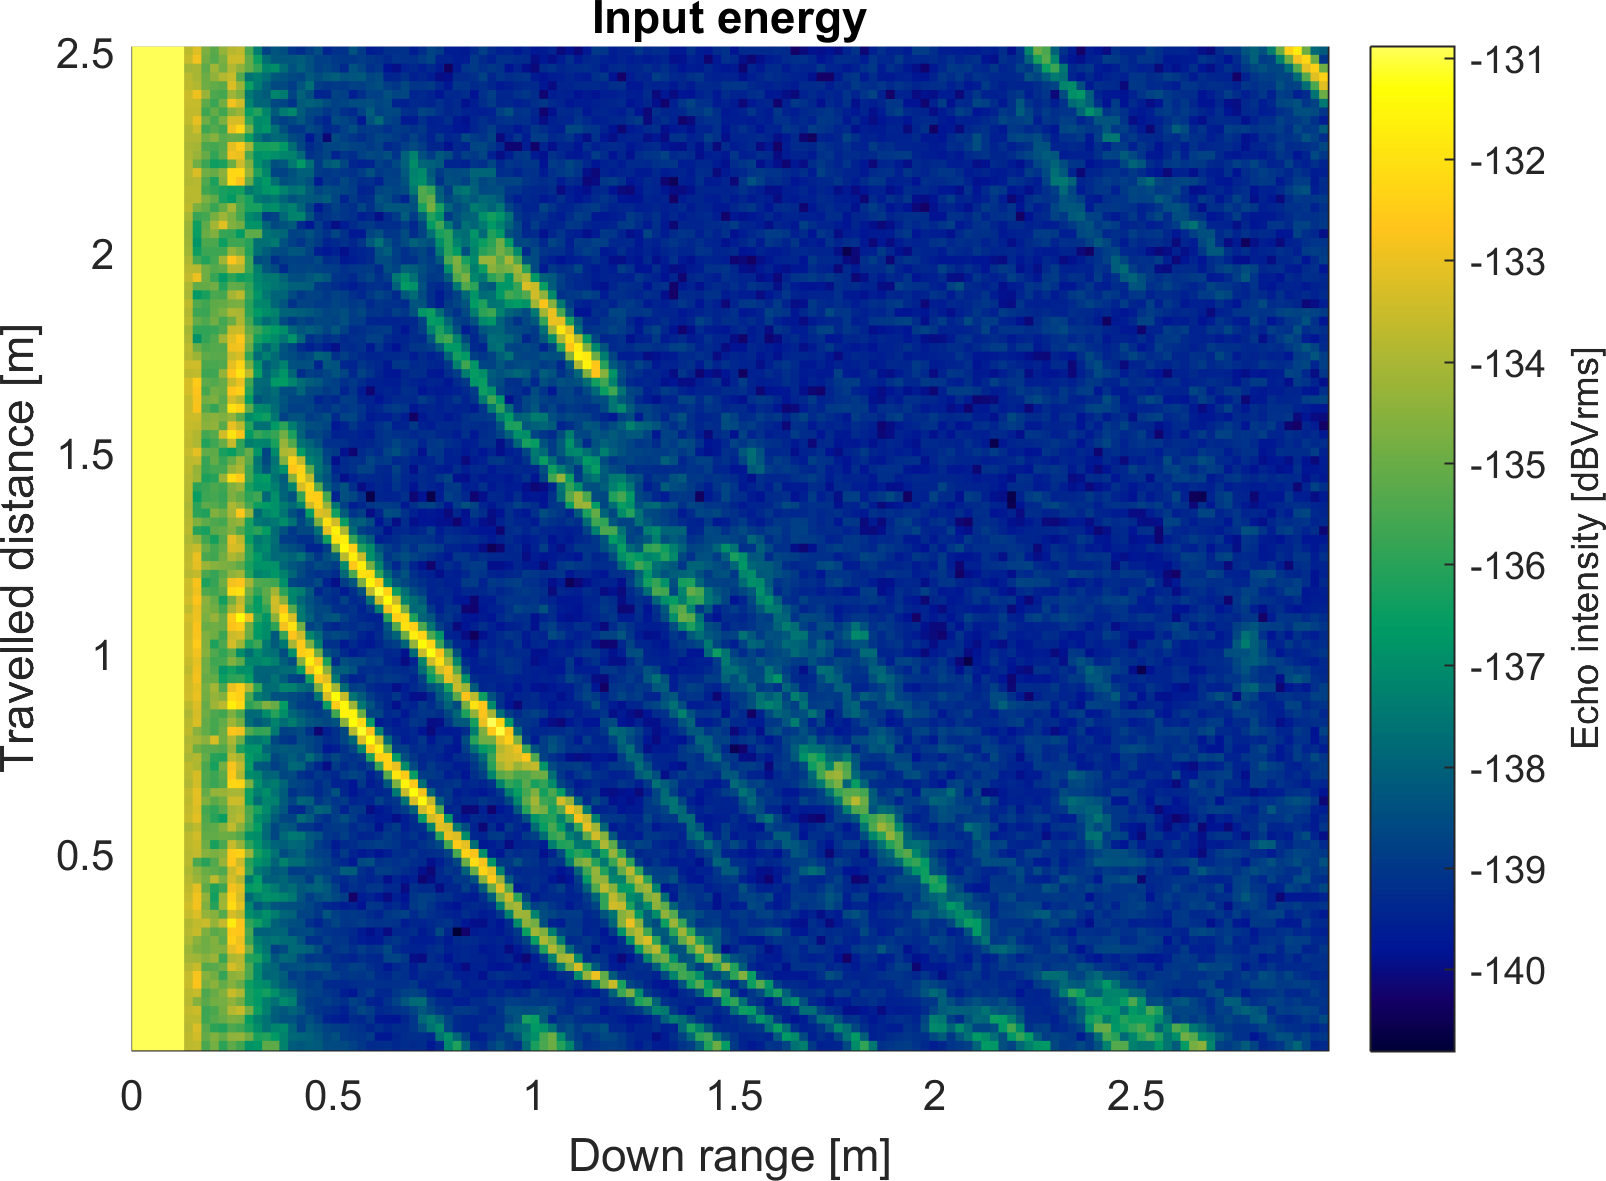
\includegraphics[width=\linewidth,max height=.475\textheight]{gfx/results/nirvana_input.png}
    \end{subfigure}%
    \hfill%
    \begin{subfigure}[t]{0.475\linewidth}
        \centering
        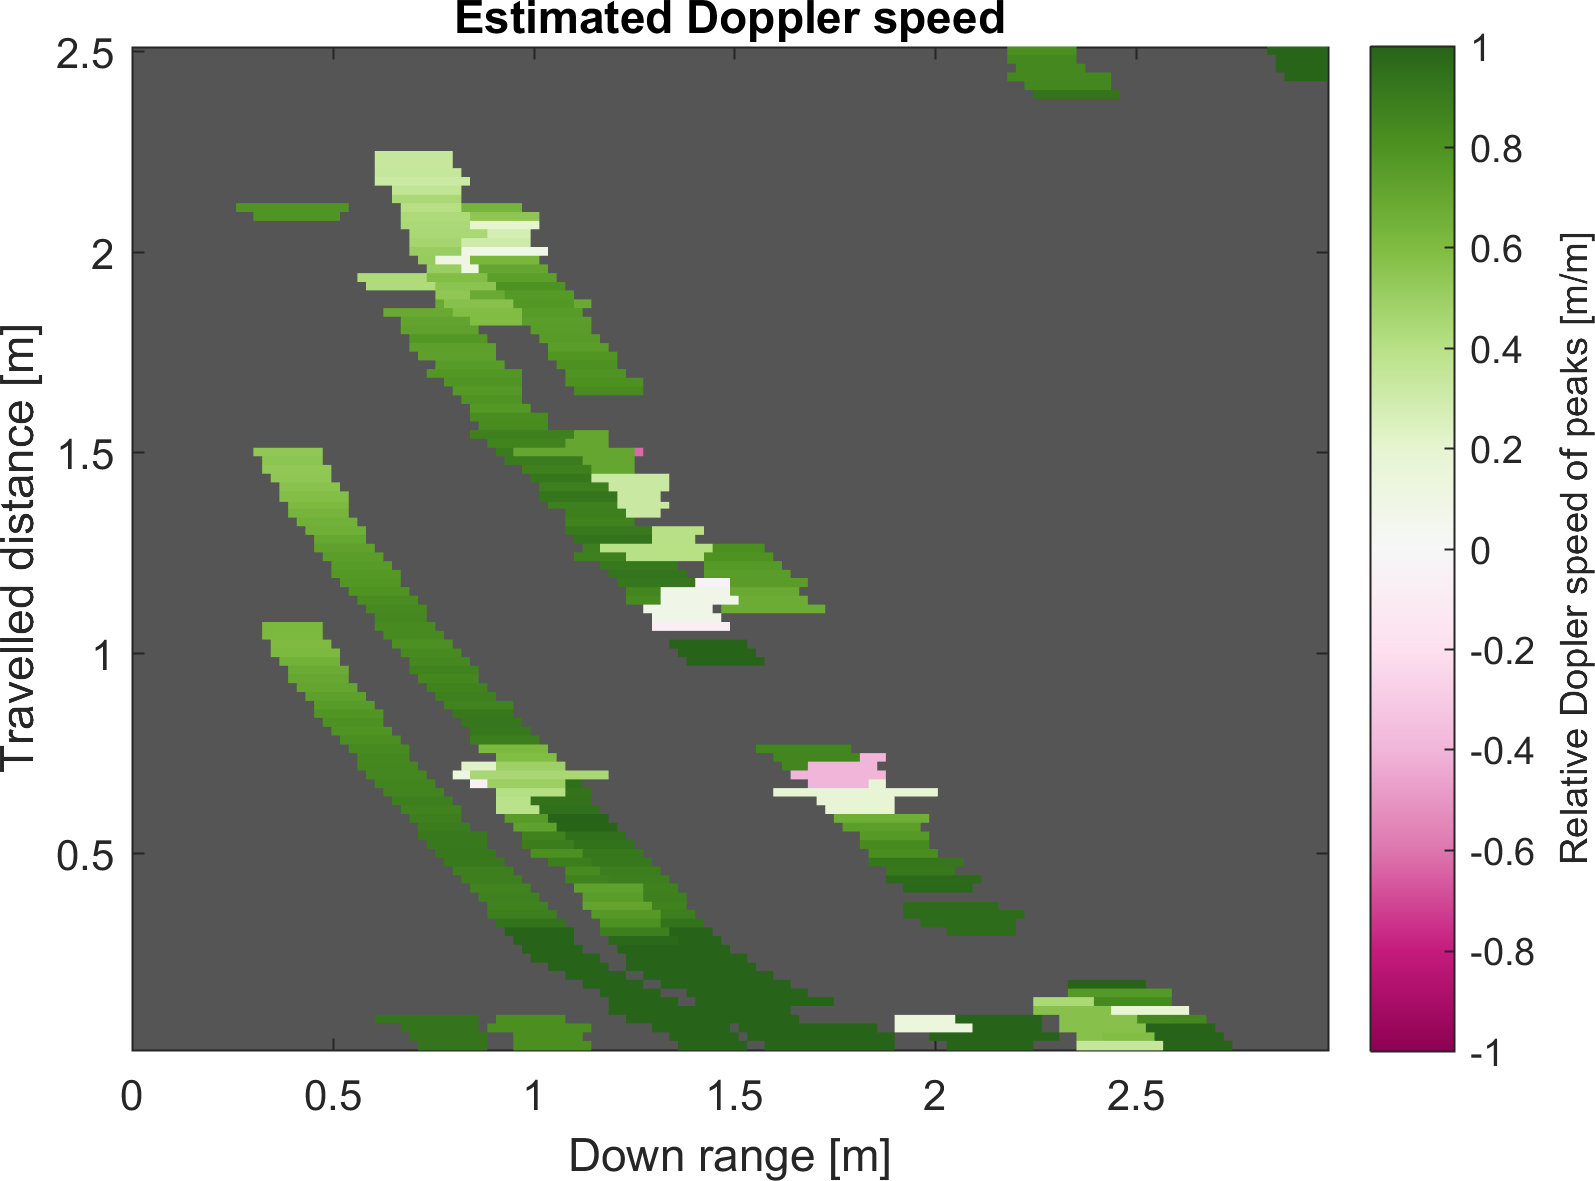
\includegraphics[width=\linewidth,max height=.475\textheight]{gfx/results/nirvana_doppler.png}
    \end{subfigure}\bigskip\\
    \begin{subfigure}[t]{0.475\linewidth}  
        \centering 
        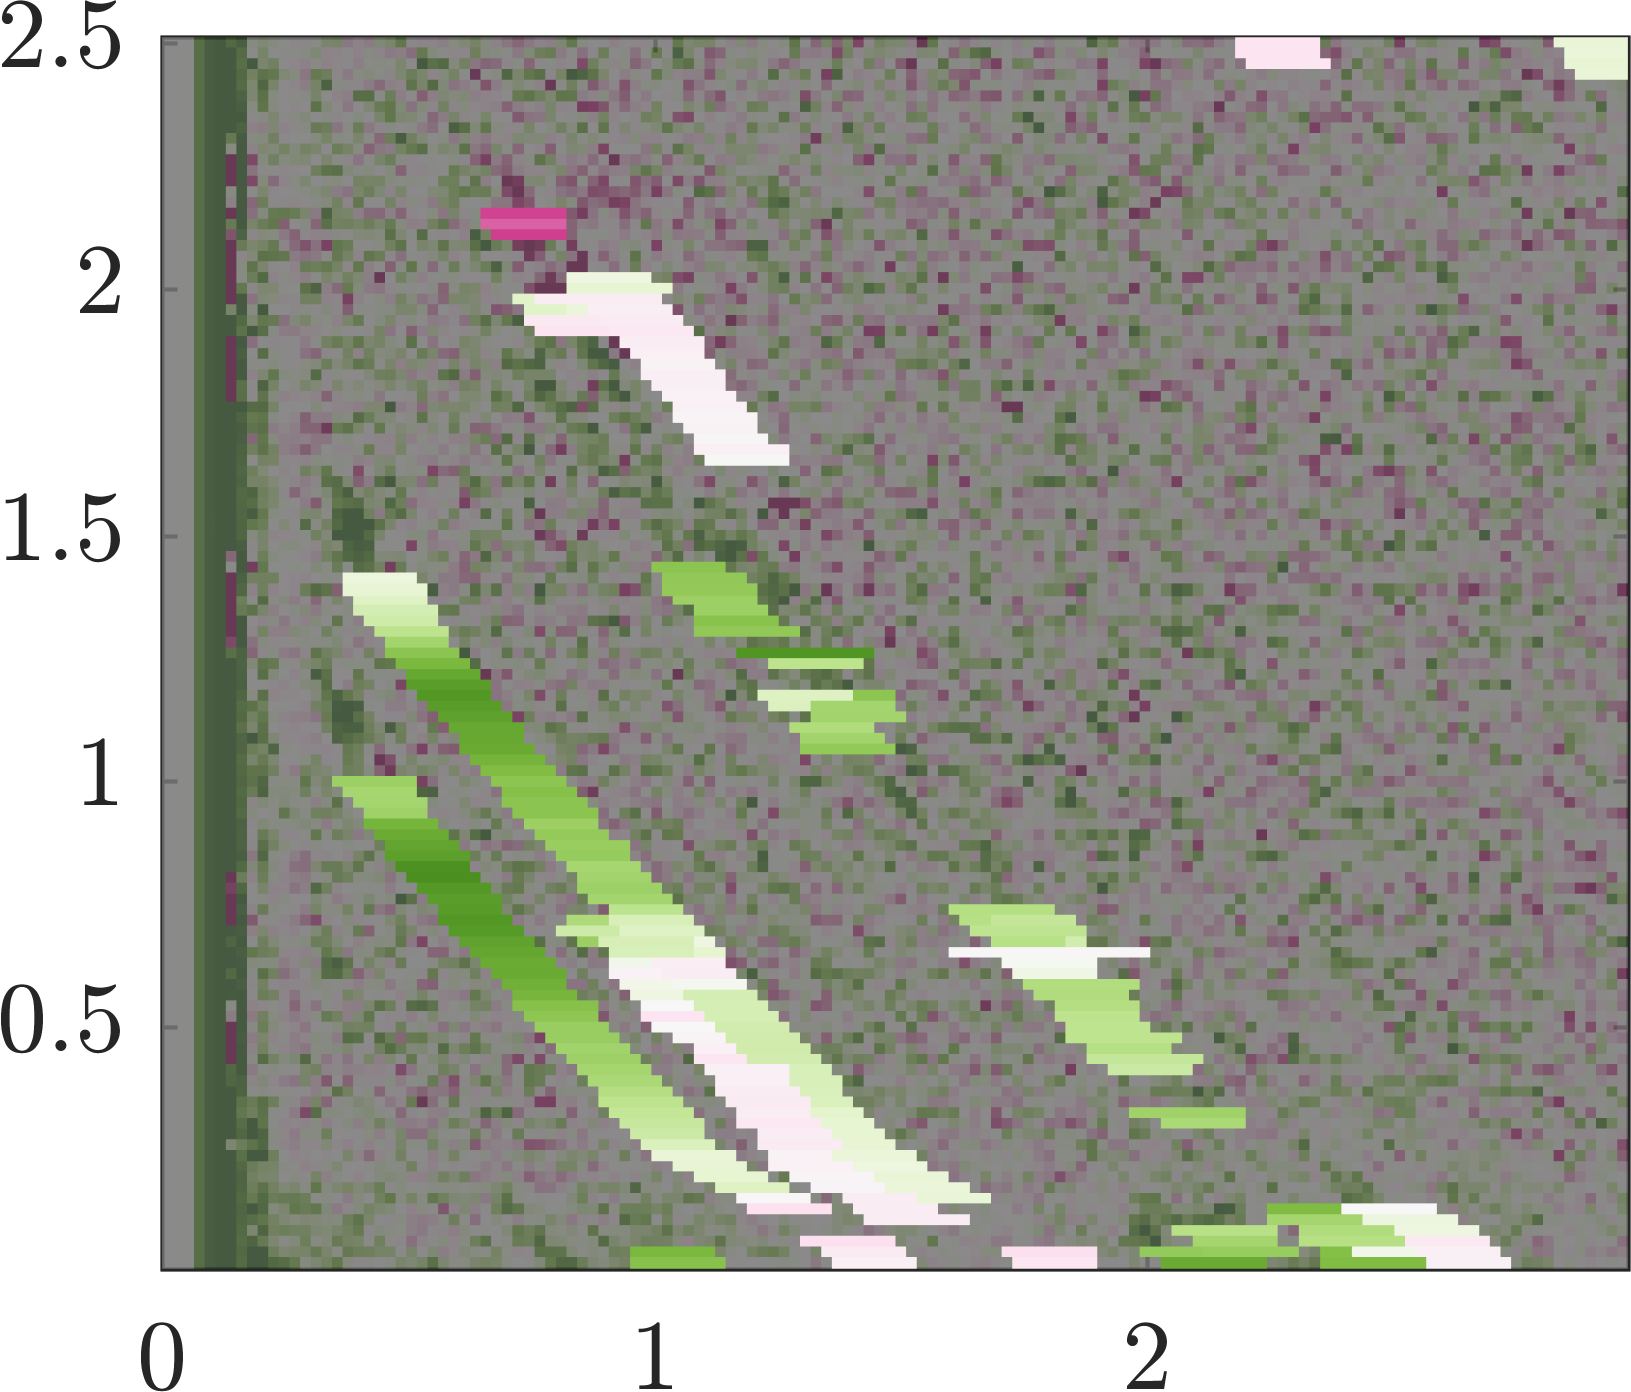
\includegraphics[width=\linewidth,max height=.475\textheight]{gfx/results/nirvana_doa.png}
    \end{subfigure}%
    \hfill%
    \begin{subfigure}[t]{0.475\linewidth}   
        \centering 
        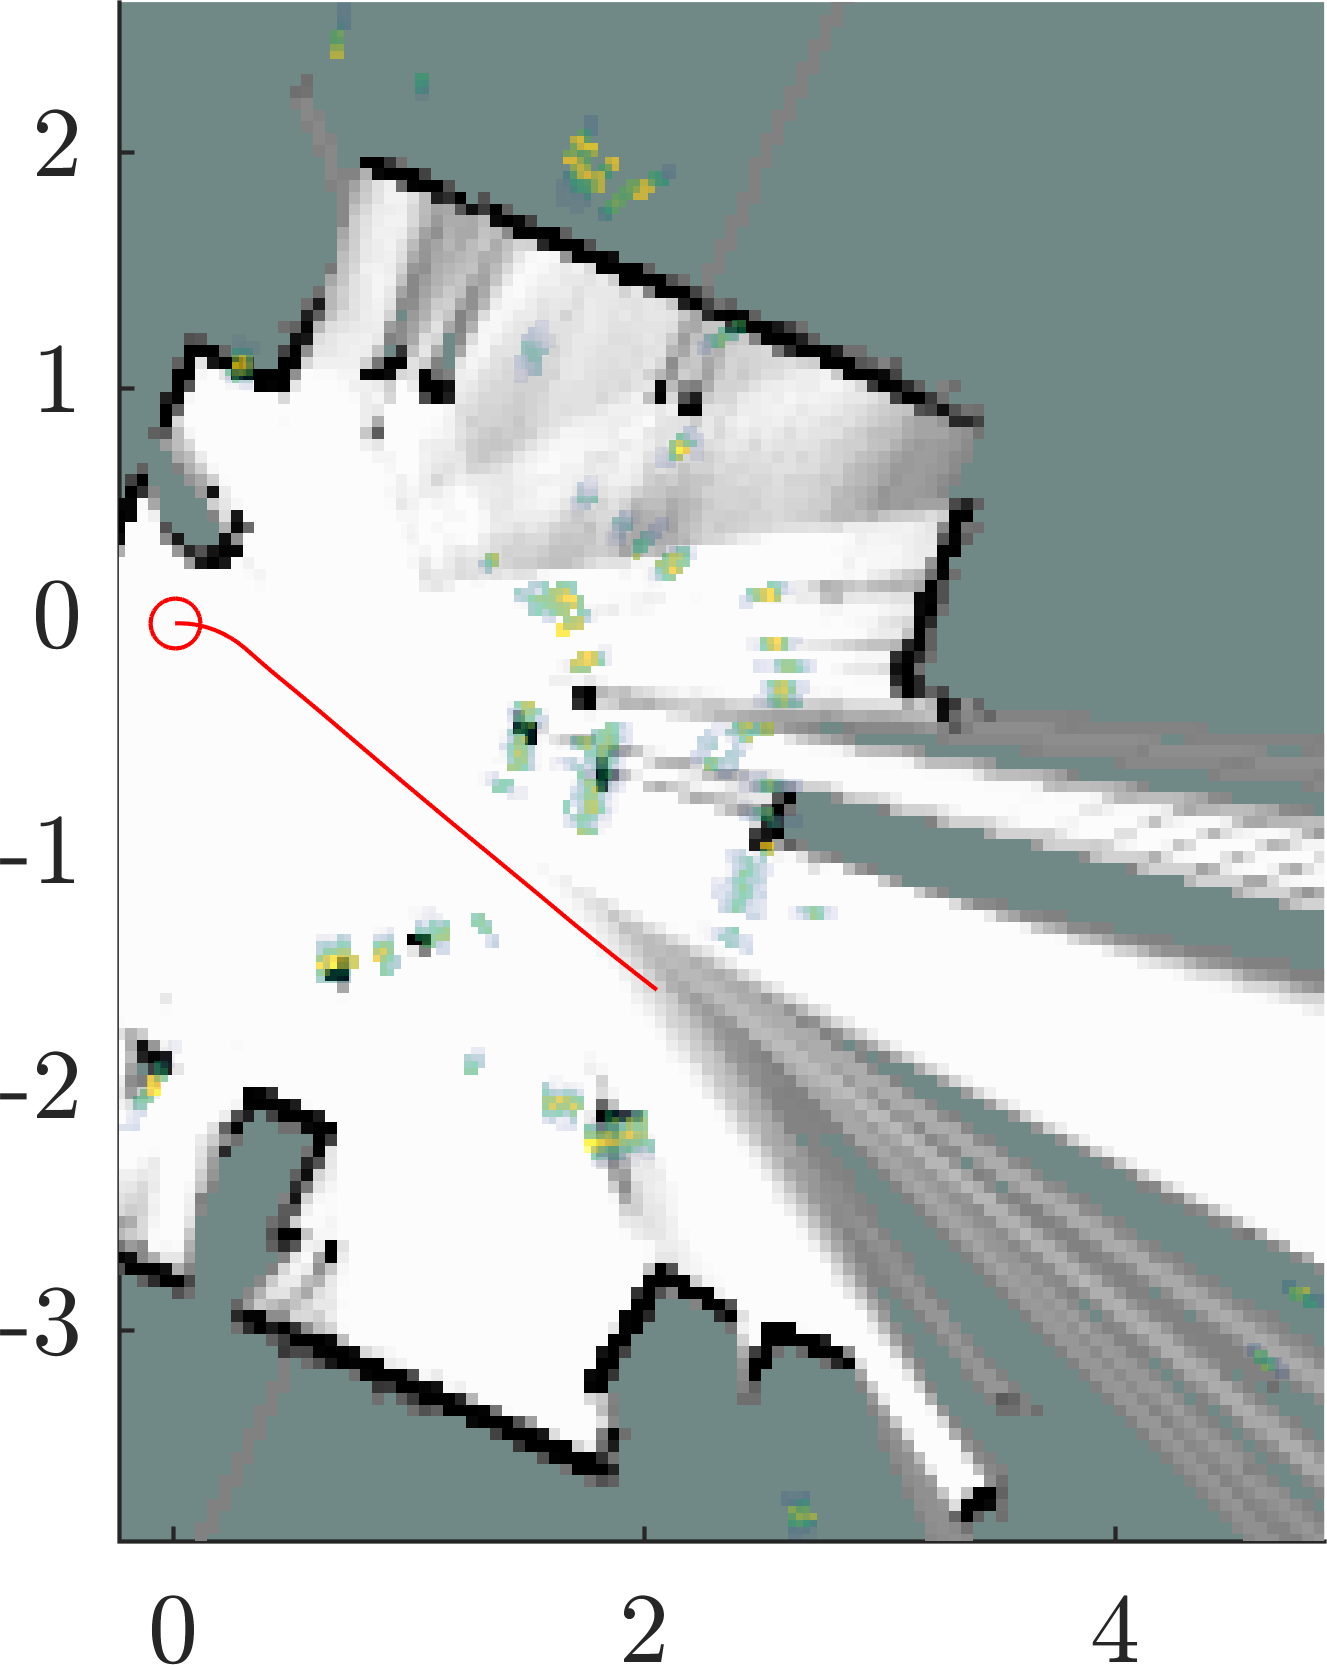
\includegraphics[width=\linewidth,max height=.475\textheight]{gfx/results/nirvana_map.png}
    \end{subfigure}%
    \caption{Nirvana scan}
\end{figure}

\begin{figure}[htbp]
    \centering
    \begin{subfigure}[t]{0.475\linewidth}
        \centering
        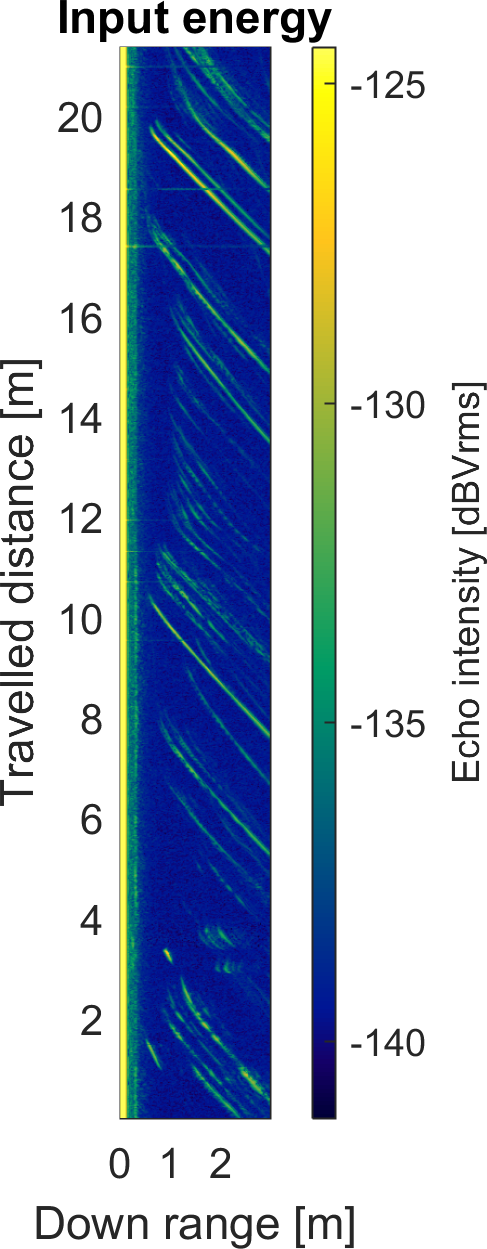
\includegraphics[width=\linewidth,max height=.475\textheight]{gfx/results/orbit_input.png}
    \end{subfigure}%
    \hfill%
    \begin{subfigure}[t]{0.475\linewidth}
        \centering
        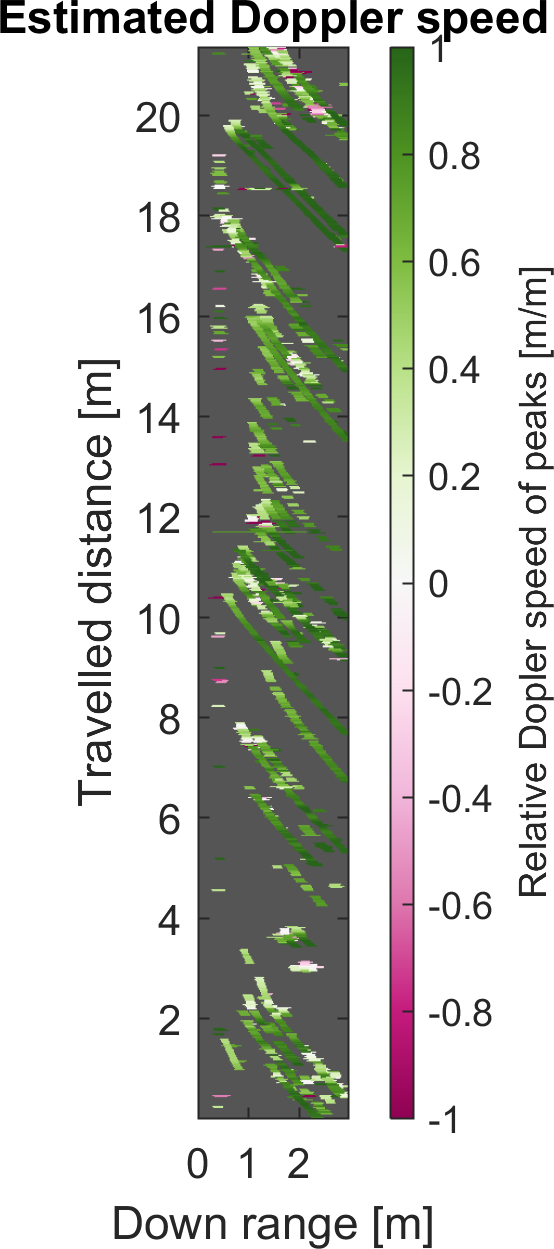
\includegraphics[width=\linewidth,max height=.475\textheight]{gfx/results/orbit_doppler.png}
    \end{subfigure}\bigskip\\
    \begin{subfigure}[t]{0.475\linewidth}  
        \centering 
        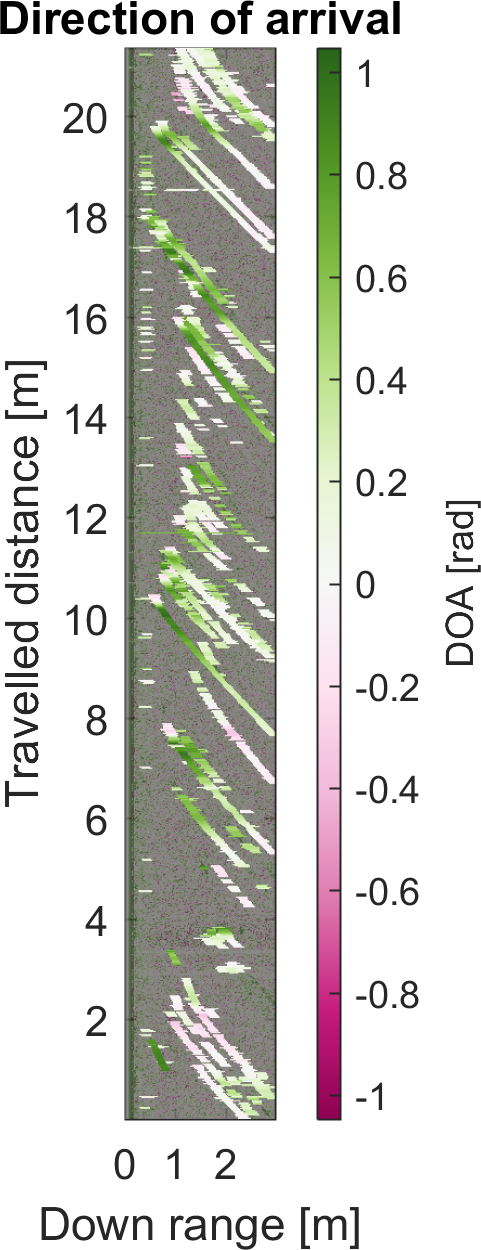
\includegraphics[width=\linewidth,max height=.475\textheight]{gfx/results/orbit_doa.png}
    \end{subfigure}%
    \hfill%
    \begin{subfigure}[t]{0.475\linewidth}   
        \centering 
        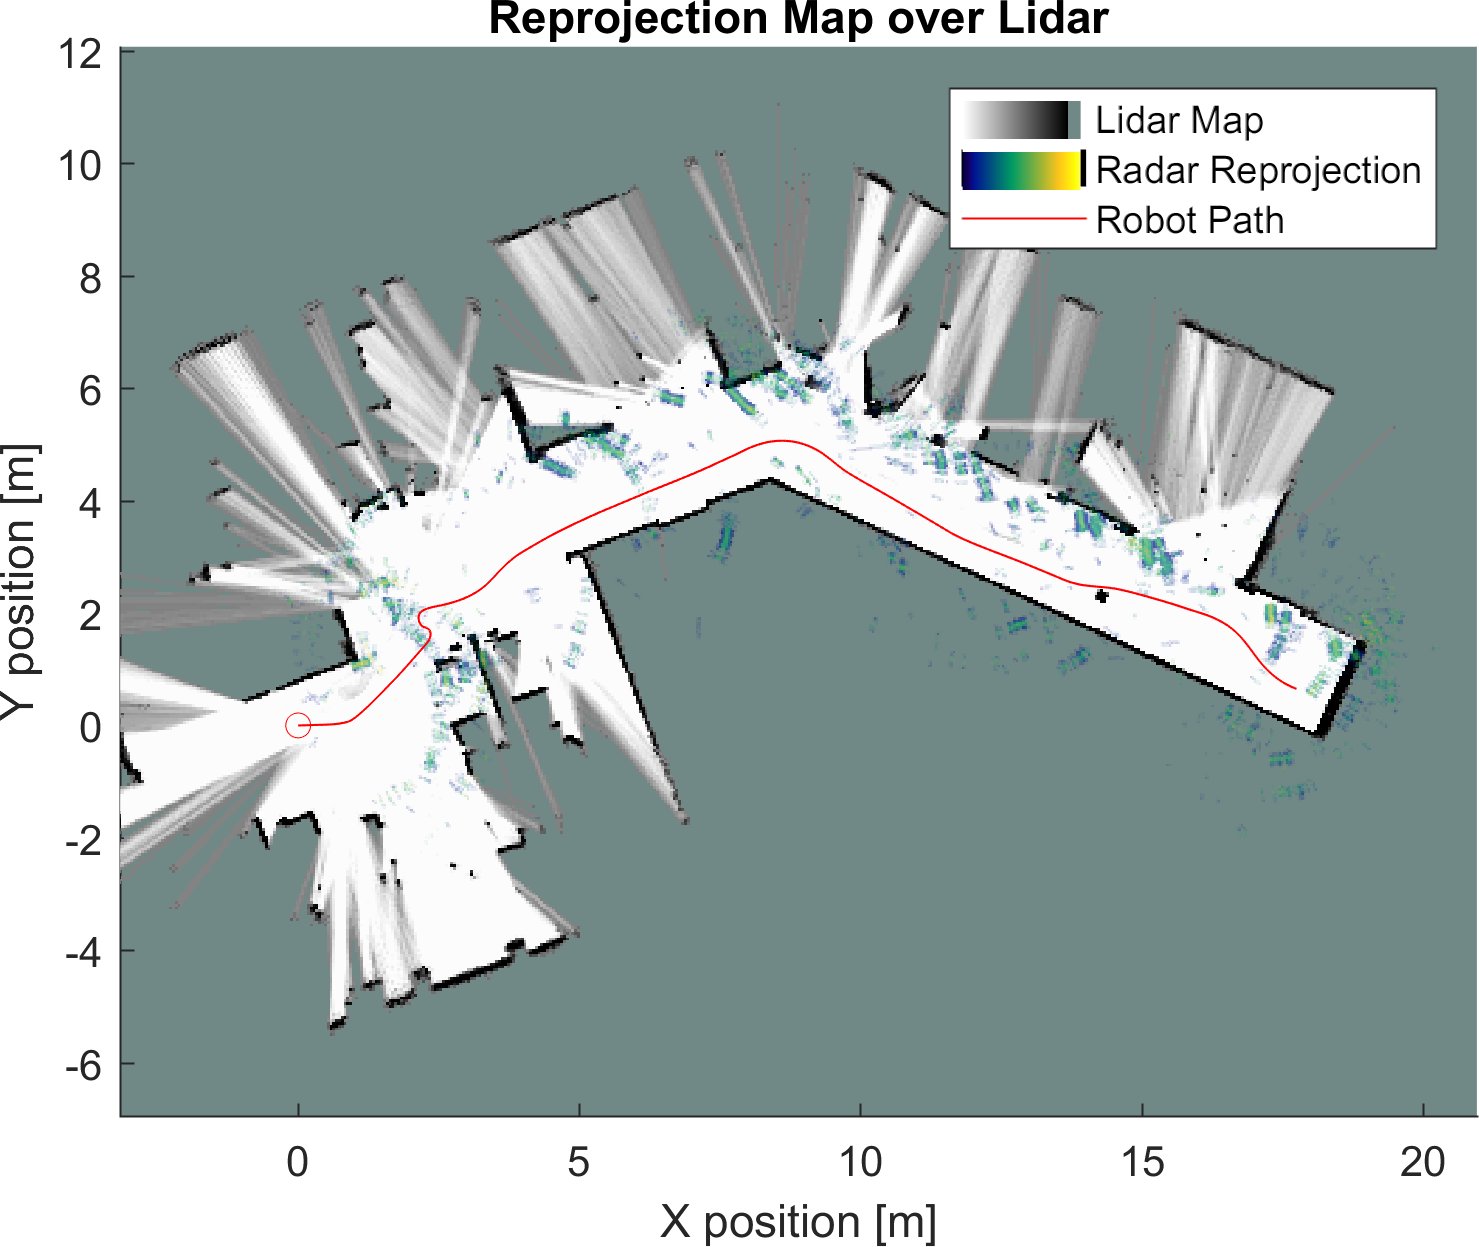
\includegraphics[width=\linewidth,max height=.475\textheight]{gfx/results/orbit_map.png}
    \end{subfigure}%
    \caption{Orbit scan}
\end{figure}

\begin{figure}[htbp]
    \centering
    \begin{subfigure}[t]{0.475\linewidth}
        \centering
        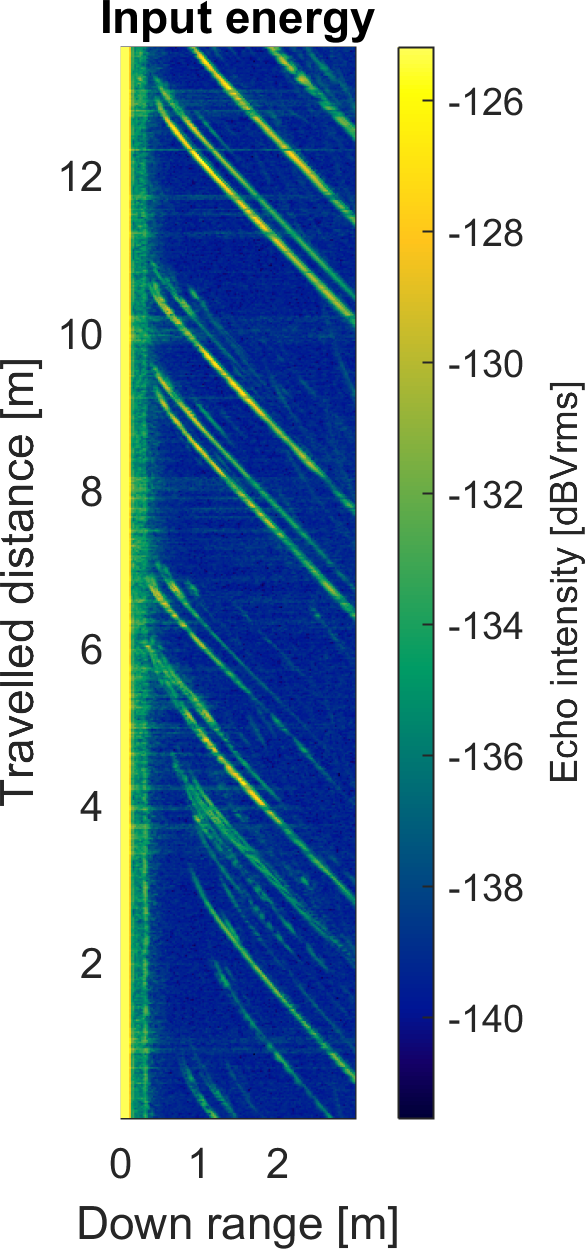
\includegraphics[width=\linewidth,max height=.475\textheight]{gfx/results/publicrestroom_input.png}
    \end{subfigure}%
    \hfill%
    \begin{subfigure}[t]{0.475\linewidth}
        \centering
        \includegraphics[width=\linewidth,max height=.475\textheight]{gfx/results/publicrestroom_doppler.png}
    \end{subfigure}\bigskip\\
    \begin{subfigure}[t]{0.475\linewidth}  
        \centering 
        \includegraphics[width=\linewidth,max height=.475\textheight]{gfx/results/publicrestroom_doa.png}
    \end{subfigure}%
    \hfill%
    \begin{subfigure}[t]{0.475\linewidth}   
        \centering 
        \includegraphics[width=\linewidth,max height=.475\textheight]{gfx/results/publicrestroom_map.png}
    \end{subfigure}%
    \caption{Public Restroom scan}
    \label{fig:res_p}
\end{figure}

\begin{figure}[htbp]
    \centering
    \begin{subfigure}[t]{0.475\linewidth}
        \centering
        \includegraphics[width=\linewidth,max height=.475\textheight]{gfx/results/queue_input.png}
    \end{subfigure}%
    \hfill%
    \begin{subfigure}[t]{0.475\linewidth}
        \centering
        \includegraphics[width=\linewidth,max height=.475\textheight]{gfx/results/queue_doppler.png}
    \end{subfigure}\bigskip\\
    \begin{subfigure}[t]{0.475\linewidth}  
        \centering 
        \includegraphics[width=\linewidth,max height=.475\textheight]{gfx/results/queue_doa.png}
    \end{subfigure}%
    \hfill%
    \begin{subfigure}[t]{0.475\linewidth}   
        \centering 
        \includegraphics[width=\linewidth,max height=.475\textheight]{gfx/results/queue_map.png}
    \end{subfigure}%
    \caption{Queue scan}
    \label{fig:res_q}
\end{figure}

\begin{figure}[htbp]
    \centering
    \begin{subfigure}[t]{0.475\linewidth}
        \centering
        \includegraphics[width=\linewidth,max height=.475\textheight]{gfx/results/racetrack_input.png}
    \end{subfigure}%
    \hfill%
    \begin{subfigure}[t]{0.475\linewidth}
        \centering
        \includegraphics[width=\linewidth,max height=.475\textheight]{gfx/results/racetrack_doppler.png}
    \end{subfigure}\bigskip\\
    \begin{subfigure}[t]{0.475\linewidth}  
        \centering 
        \includegraphics[width=\linewidth,max height=.475\textheight]{gfx/results/racetrack_doa.png}
    \end{subfigure}%
    \hfill%
    \begin{subfigure}[t]{0.475\linewidth}   
        \centering 
        \includegraphics[width=\linewidth,max height=.475\textheight]{gfx/results/racetrack_map.png}
    \end{subfigure}%
    \caption{Racetrack scan}
    \label{fig:res_r}
\end{figure}

\begin{figure}[htbp]
    \centering
    \begin{subfigure}[t]{0.475\linewidth}
        \centering
        \includegraphics[width=\linewidth,max height=.475\textheight]{gfx/results/sauna_input.png}
    \end{subfigure}%
    \hfill%
    \begin{subfigure}[t]{0.475\linewidth}
        \centering
        \includegraphics[width=\linewidth,max height=.475\textheight]{gfx/results/sauna_doppler.png}
    \end{subfigure}\bigskip\\
    \begin{subfigure}[t]{0.475\linewidth}  
        \centering 
        \includegraphics[width=\linewidth,max height=.475\textheight]{gfx/results/sauna_doa.png}
    \end{subfigure}%
    \hfill%
    \begin{subfigure}[t]{0.475\linewidth}   
        \centering 
        \includegraphics[width=\linewidth,max height=.475\textheight]{gfx/results/sauna_map.png}
    \end{subfigure}%
    \caption{Sauna scan}
    \label{fig:res_s}
\end{figure}

\begin{figure}[htbp]
    \centering
    \begin{subfigure}[t]{0.475\linewidth}
        \centering
        \includegraphics[width=\linewidth,max height=.475\textheight]{gfx/results/torturechamber_input.png}
    \end{subfigure}%
    \hfill%
    \begin{subfigure}[t]{0.475\linewidth}
        \centering
        \includegraphics[width=\linewidth,max height=.475\textheight]{gfx/results/torturechamber_doppler.png}
    \end{subfigure}\bigskip\\
    \begin{subfigure}[t]{0.475\linewidth}  
        \centering 
        \includegraphics[width=\linewidth,max height=.475\textheight]{gfx/results/torturechamber_doa.png}
    \end{subfigure}%
    \hfill%
    \begin{subfigure}[t]{0.475\linewidth}   
        \centering 
        \includegraphics[width=\linewidth,max height=.475\textheight]{gfx/results/torturechamber_map.png}
    \end{subfigure}%
    \caption{Torture Chamber scan}
\end{figure}

\begin{figure}[htbp]
    \centering
    \begin{subfigure}[t]{0.475\linewidth}
        \centering
        \includegraphics[width=\linewidth,max height=.475\textheight]{gfx/results/underground_input.png}
    \end{subfigure}%
    \hfill%
    \begin{subfigure}[t]{0.475\linewidth}
        \centering
        \includegraphics[width=\linewidth,max height=.475\textheight]{gfx/results/underground_doppler.png}
    \end{subfigure}\bigskip\\
    \begin{subfigure}[t]{0.475\linewidth}  
        \centering 
        \includegraphics[width=\linewidth,max height=.475\textheight]{gfx/results/underground_doa.png}
    \end{subfigure}%
    \hfill%
    \begin{subfigure}[t]{0.475\linewidth}   
        \centering 
        \includegraphics[width=\linewidth,max height=.475\textheight]{gfx/results/underground_map.png}
    \end{subfigure}%
    \caption{Underground scan}
\end{figure}

\begin{figure}[htbp]
    \centering
    \begin{subfigure}[t]{0.475\linewidth}
        \centering
        \includegraphics[width=\linewidth,max height=.475\textheight]{gfx/results/virtualreality_input.png}
    \end{subfigure}%
    \hfill%
    \begin{subfigure}[t]{0.475\linewidth}
        \centering
        \includegraphics[width=\linewidth,max height=.475\textheight]{gfx/results/virtualreality_doppler.png}
    \end{subfigure}\bigskip\\
    \begin{subfigure}[t]{0.475\linewidth}  
        \centering 
        \includegraphics[width=\linewidth,max height=.475\textheight]{gfx/results/virtualreality_doa.png}
    \end{subfigure}%
    \hfill%
    \begin{subfigure}[t]{0.475\linewidth}   
        \centering 
        \includegraphics[width=\linewidth,max height=.475\textheight]{gfx/results/virtualreality_map.png}
    \end{subfigure}%
    \caption{Virtual Reality scan}
\end{figure}

\begin{figure}[htbp]
    \centering
    \begin{subfigure}[t]{0.475\linewidth}
        \centering
        \includegraphics[width=\linewidth,max height=.475\textheight]{gfx/results/washroom_input.png}
    \end{subfigure}%
    \hfill%
    \begin{subfigure}[t]{0.475\linewidth}
        \centering
        \includegraphics[width=\linewidth,max height=.475\textheight]{gfx/results/washroom_doppler.png}
    \end{subfigure}\bigskip\\
    \begin{subfigure}[t]{0.475\linewidth}  
        \centering 
        \includegraphics[width=\linewidth,max height=.475\textheight]{gfx/results/washroom_doa.png}
    \end{subfigure}%
    \hfill%
    \begin{subfigure}[t]{0.475\linewidth}   
        \centering 
        \includegraphics[width=\linewidth,max height=.475\textheight]{gfx/results/washroom_map.png}
    \end{subfigure}%
    \caption{Washroom scan}
\end{figure}

\begin{figure}[htbp]
    \centering
    \begin{subfigure}[t]{0.475\linewidth}
        \centering
        \includegraphics[width=\linewidth,max height=.475\textheight]{gfx/results/xrayroom_input.png}
    \end{subfigure}%
    \hfill%
    \begin{subfigure}[t]{0.475\linewidth}
        \centering
        \includegraphics[width=\linewidth,max height=.475\textheight]{gfx/results/xrayroom_doppler.png}
    \end{subfigure}\bigskip\\
    \begin{subfigure}[t]{0.475\linewidth}  
        \centering 
        \includegraphics[width=\linewidth,max height=.475\textheight]{gfx/results/xrayroom_doa.png}
    \end{subfigure}%
    \hfill%
    \begin{subfigure}[t]{0.475\linewidth}   
        \centering 
        \includegraphics[width=\linewidth,max height=.475\textheight]{gfx/results/xrayroom_map.png}
    \end{subfigure}%
    \caption{X-Ray Room scan}
\end{figure}

\begin{figure}[htbp]
    \centering
    \begin{subfigure}[t]{0.475\linewidth}
        \centering
        \includegraphics[width=\linewidth,max height=.475\textheight]{gfx/results/y_input.png}
    \end{subfigure}%
    \hfill%
    \begin{subfigure}[t]{0.475\linewidth}
        \centering
        \includegraphics[width=\linewidth,max height=.475\textheight]{gfx/results/y_doppler.png}
    \end{subfigure}\bigskip\\
    \begin{subfigure}[t]{0.475\linewidth}  
        \centering 
        \includegraphics[width=\linewidth,max height=.475\textheight]{gfx/results/y_doa.png}
    \end{subfigure}%
    \hfill%
    \begin{subfigure}[t]{0.475\linewidth}   
        \centering 
        \includegraphics[width=\linewidth,max height=.475\textheight]{gfx/results/y_map.png}
    \end{subfigure}%
    \caption{Y (Is There A Cable On The Floor) scan}
\end{figure}




